\documentclass[12pt, twoside]{report}
\usepackage[utf8]{inputenc}

\usepackage[a4paper,top=2.5cm,bottom=2.5cm,left=3cm,right=2.5cm]{geometry}

%\usepackage[parfill]{parskip}    % Begin paragraphs with empty line instead of indent
\usepackage{graphicx}             % Use pdf, png, jpg or eps with pdflatex (eps in DVI mode)
                                  % TeX automatically converts eps --> pdf in pdflatex
\usepackage{wrapfig}

\usepackage{amssymb}
%\usepackage{ebgaramond}

\usepackage[onehalfspacing]{setspace}
\setlength{\parskip}{0cm}

\usepackage{nameref}
\usepackage[colorlinks,linkcolor=magenta]{hyperref} % set link colour to magenta?

\usepackage[font=small,labelfont=bf]{caption}

\usepackage{listings}
\usepackage{xcolor}

\usepackage{booktabs}
\usepackage{tabularx}

%\usepackage{type1cm}
%\usepackage{lettrine}

% FUNCTIONS --------------------------------------------------------

% Use \rurl{} to create a link without displaying https://
\newcommand*{\rurl}[1]{\small{\href{https://#1}{\nolinkurl{#1}}}}

% Use \fullref{} to fully reference a \label{}, e.g.
%   Latex -> For more details, read \fullref{chap:methods}.
%   PDF   -> For more details, read chapter 4: \textbf{Methods}.
\newcommand*{\fullref}[1]{\hyperref[{#1}]{\autoref*{#1}: \textbf{\nameref*{#1}}}}

% CODE STYLING -----------------------------------------------------

\definecolor{codegreen}{rgb}{0,0.6,0}
\definecolor{codegray}{rgb}{0.5,0.5,0.5}
\definecolor{codepurple}{rgb}{0.58,0,0.82}
\definecolor{backcolour}{rgb}{0.95,0.95,0.92}

\lstdefinestyle{mystyle}{
    backgroundcolor=\color{backcolour},   
    commentstyle=\color{codegreen},
    keywordstyle=\color{magenta},
    numberstyle=\tiny\color{codegray},
    stringstyle=\color{codepurple},
    basicstyle=\ttfamily\footnotesize,
    breakatwhitespace=false,         
    breaklines=true,                 
    captionpos=b,                    
    keepspaces=true,                 
    numbers=left,                    
    numbersep=5pt,                  
    showspaces=false,                
    showstringspaces=false,
    showtabs=false
}

\lstset{style=mystyle}

% ------------------------------------------------------------------

\begin{document}

\begin{titlepage}
    \begin{center}
        \vspace*{-.2cm}
        UNIVERSIDADE DE LISBOA
        
        Faculdade de Medicina
        
        
\includegraphics[width=0.6\textwidth]{images/logo/ulisboa}
        
        \vspace{1.8cm}
        Thesis Title
        
        \vspace{0.5cm}
        Thesis Subtitle
            
        \vspace{0.9cm}            
        Nuno Daniel Saraiva Agostinho
    \end{center}

    \vspace{0.9cm}
    Orientador: Prof. Doutor Nuno Luís Barbosa Morais
    
    \vspace{2.2cm}
    \begin{center}
        Documento provisório
        
        Tese especialmente elaborada para obtenção do grau de Doutor em\\
        Ciências Biomédicas, Ramo da Biologia Computacional
            
        \vfill
        2021
        \vspace{.7cm}    
    \end{center}
\end{titlepage}

\pagenumbering{roman}
\tableofcontents

\chapter*{Resumo}
\addcontentsline{toc}{chapter}{Resumo}

\chapter*{Summary}
\addcontentsline{toc}{chapter}{Summary}
Abstract goes here

\chapter*{Acknowledgements}
\addcontentsline{toc}{chapter}{Acknowledgements}

\listoffigures
\addcontentsline{toc}{chapter}{List of Figures}

\listoftables
\addcontentsline{toc}{chapter}{List of Tables}

% !TEX root = ../PhD Thesis.tex
\chapter{Introduction}
\pagenumbering{arabic}

\section{On the origin of life}

This is the story of my PhD, a personal journey like no other I have faced before. To follow my story, we have to rewind back to years ago. Billions and billions of years ago. Once upon a time there was a violent, harsh and unwelcoming planet among countless others. Earth was lifeless. But as millions of years went by, it started being home to a complex recipe whose special sauce is still being studied to this day: the primordial soup. These were the perfect conditions for a young, 500-million-year-old planet to brew life.

And what is life? Although this question is not easy to answer, living organisms as we know them are complex, carbon-based systems composed of nucleic acids, proteins, carbohydrates and lipids. Together with some smaller molecules, these molecules are known as biomolecules and are crucial for the survival of living organisms.

Amongst those biomolecules, two are particularly relevant to my story: proteins and nucleic acids. Proteins have many important functions in an organism, including catalysing chemical reactions (enzymes), signalling cellular processes (hormones) and playing a role in the immune system (antigens). Regarding nucleic acids, deoxyribonucleic acid (DNA) stores the genetic data, the blueprint required to generate the majority of the vital molecules in the cell, including ribonucleic acid (RNA) molecules for protein synthesis and regulation.
% messenger RNAs (mRNA) are coding RNAs whose sequence is used as a template to create new proteins, transfer RNAs (tRNA) carry amino acids to generate proteins and ribosomal RNAs (rRNA) are the major components of the ribosome, the protein synthesis machinery. Other non-coding RNAs (long non-coding RNAs, small interfering RNAs, micro RNAs, etc.) have further regulatory roles in the cell.

% Miller-Urey experiment
% But how did all this complexity emerged from the primordial soup? The primitive Earth's  atmosphere was rich in inorganic compounds (the exact ones are still up to debate). Together with 

One possibility for the origin of life is based on the idea of %that ribonucleic acid (RNA) was the molecule that made (modern\footnote{Other transitory living organisms that precede RNA-based living organisms are also hypothesised.}) life possible:
the RNA world, an hypothesis in which self-replicating RNA evolutionarily predates DNA and proteins \cite{gilbert:1986td}. After all, RNA molecules are able to store genetic information like DNA and some can even catalyse life-critical chemical reactions like enzymes, making RNA a prime candidate for life to take its first steps \cite{gilbert:1986td}. Later on, these specific functions may have been overtaken by enzymes, proteins that were more effective as reaction catalysers, and DNA, a more stable and less error-prone nucleic acid to store genetic information \cite{gilbert:1986td}.

% Re-creating the RNA world, 1995 review, https://www.cell.com/action/showPdf?pii=S0960-9822%2895%2900205-3

% Progenote: the last common ancestor of modern life

% Gene expression

\section{On the origin of species}

Throughout millions of years, evolution continued.

\section{On nucleic acids and protein synthesis}

It was in the year of 1869 that Friedrich Miescher isolated a mysterious, protein-like substance that he named \emph{nuclein}, found in the cell nucleus of diverse vertebrates. Miescher's work led him to believe that an increase in nuclein could be associated with the first stages of cell division in proliferating tissues \cite{dahm:2005wx}. Nuclein was renamed nucleic acid in 1889 \cite{dahm:2005wx}.

% 1885-1901, isolated the 5 nucleobases that constitute DNA + RNA

% 1902–1909: Archibald Garrod proposes that genetic defects result in the loss of enzymes and hereditary metabolic diseases.

Contrary to the consensus in the first decades of the 20th century, Boveri and Sutton theorised that the chromosomes -- not proteins as previously thought -- carried genetic information \cite{sutton:1902tx,dahm:2005wx}. According to Sutton:

\begin{displayquote}[\cite{sutton:1902tx}]
the association of paternal and maternal chromosomes in pairs and their subsequent separation during the reducing division (...) may constitute the physical basis of the Mendelian law of heredity.
\end{displayquote}

The Boveri-Sutton chromosome theory of genetic inheritance followed Gregor Mendel's controversial \cite{} work in 1865 \cite{sutton:1902tx} and was later supported by fruit fly experiments from an initially skeptic \cite{} Thomas Morgan \cite{morgan:1915tw}. In 1915, Morgan and colleagues published a textbook with their findings describing genetic dominance, sex inheritance and chromosomal crossover. One chapter was provokingly titled \emph{The Chromosomes as Bearers of Hereditary Material} \cite{morgan:1915tw}.

% 1928: Frederick Griffith postulates that a “transforming principle” permits properties from one type of bacteria (heat-inactivated virulent Streptococcus pneumoniae) to be transferred to another (live nonvirulent Streptococcus pneumoniae).

% Around 1930s, Phoebus Levene identified the four DNA nucleotides (adenine, cytosine, guanine, and thymine), as well as the sugar-phosphate backbone \cite{levene:1929ug}. % confirm if in this paper

% In 1933, Jean Brachet found evidence of \emph{thymus nucleic acid} (nowadays known as DNA) in the cell nucleus and of \emph{yeast nucleic acid} (RNA) in the cytoplasm\footnote{At the time, \emph{thymus nucleic acid} was thought to be a nucleic acid from animals (specially found in the thymus, hence its name) and \emph{yeast nucleic acid} from plants.}.

Although the word \emph{gene} was popularly used since being coined by Johannsen in 1909 to abstractly refer to Mendelian factors of inheritance (i.e. the units of heredity) \cite{}, Demerec tried to define its concept in his 1933 publication, \emph{What is a Gene?}: % Demerec also depicts a tentative structure of DNA

\begin{displayquote}[\cite{}]
(...) [A gene] is a minute organic particle, capable of reproduction, located in a chromosome and responsible for the transmission of a hereditary characteristic.
\end{displayquote}

Later in 1941, George Beadle and Edward Tatum hypothesised that each gene is responsible for producing a specific enzyme and demonstrated that radiation-induced mutations could alter the resulting enzyme.

% 1949: Colette and Roger Vendrely and André Boivin discover that the nuclei of germ cells contain half the amount of DNA that is found in somatic cells. This parallels the reduction in the number of chromosomes during gametogenesis and provides further evidence for the fact that DNA is the genetic material.

% 1952: Alfred Hershey and Martha Chase use viruses (bacteriophage T2) to confirm DNA as the genetic material by demonstrating that during infection viral DNA enters the bacteria while the viral proteins do not and that this DNA can be found in progeny virus particles.

% In 1953, the work by Watson, Crick, Rosalind Franklin, Maurice Wilkins on DNA's double helix structure
% Molecular Structure of Nucleic Acids, Watson + Crick 1953, http://dosequis.colorado.edu/Courses/MethodsLogic/papers/WatsonCrick1953.pdf

In 1955, George Palade described the ribosome as "a small particulate component of the cytoplasm" that associates with RNA in the endoplasmic reticulum membrane to perform protein synthesis \cite{palade:1955tf,jacob:1961uh}. The associated RNA was divided in two: ribosomal RNA (rRNA) that composed the ribosome itself and \emph{soluble RNA} -- transfer RNA (tRNA) --, found to carry the amino acids for protein synthesis \cite{hoagland:1958vm,jacob:1961uh}.

In 1956, the DNA polymerase is discovered, an enzyme that replicates DNA. 

In 1957, Francis Crick proposes that the genetic information flows from DNA to protein via RNA: the \emph{central dogma of molecular biology}.
% There was once a time when scientists did not all agree on the idea that nucleic acids played a role in protein synthesis.
Crick also proposed in 1958 that triplets (\emph{codons}) of the four nucleotides found in nucleic acids were necessary to produce each of the 20 universally-found types of amino acids that compose a protein \cite{crick:1958ws,crick:1961ui} and that the amino acids would be responsible for the protein's three-dimensional structure -- and consequently, its functionality \cite{crick:1958ws}.

In 1960, DNA-dependent RNA polymerase, an enzyme that synthesises RNA from DNA and common to all living organisms, was independently described.

François Jacob and Jacques Monod speculated in 1961 that ribosomal protein synthesis required an intermediate molecule with the template message to convert from DNA to protein and that would act as the \emph{messenger} \cite{jacob:1961uh,brenner:1961ve}. Unlike many of their contemporaries, they dismissed rRNA (and tRNA) molecules as the template for protein synthesis, given that they did not reflect the base composition of DNA, among other properties \cite{jacob:1961uh}. There were some published experiments on unstable RNA molecules with distinct properties from rRNA and tRNA, which Jacob and Monod proposed as relevant to their hypothesis and categorised them as messenger RNA (mRNA) \cite{jacob:1961uh,brenner:1961ve}.

% General Nature of the Genetic Code for Proteins \cite{crick:1961ui}

% Multiple ribosomes were later found to bind to a single RNA molecule (polysomes), allowing for parallelised protein synthesis \cite{warner:1963uj}.

% 1951-1965: Different kinds of tRNA were identified in the cell, each associated with a single specific amino acid. tRNAs have sequences complementary to mRNA codons and they are required for the next correct amino acid during protein synthesis.

% 1961–1966: Genetic code cracked by Robert W. Holley, Har Gobind Khorana, Heinrich Matthaei, Marshall W. Nirenberg, and colleagues: https://pubmed.ncbi.nlm.nih.gov/5322508/

1971: mRNA has a poly-A tail.

1966-75: RNA is processed by adding a polyA-tail and a 5' cap.

% 1968: The origin of the genetic code, Crick, https://doi.org/10.1016/0022-2836(68)90392-6

% Most RNAs are non-coding: ~97% in eukaryotes?

\section{On alternative splicing}

First reported in mammalian cells infected with a human adenovirus 2 \cite{berget:1977wp,chow:1977wn} and later observed in endogenous mammalian and eukaryotic genes \cite{}, mRNA-DNA hybridisation experiments suggested that genes are composed by intervening non-coding sequences. During transcription of the precursor mRNA (pre-mRNA), the non-coding sequences (introns) are excised, in contrast with the expressed segments (exons), in a process called RNA splicing \cite{berget:1977wp,chow:1977wn,gilbert:1978wr}. In 1985, a RNA-protein complex composed by U1, U2, U4, U5 and U6 small nuclear ribonucleoproteins (snRNPs) was reported crucial for RNA splicing: the spliceosome \cite{grabowski:1985vm}.

The spliceosome catalyses the removal of introns from pre-mRNA in two transesterification steps: (1) the 5' end of the intron is cleaved and united to the conserved adenosine in the branch point sequence, forming an intermediary intron lariat, and then (2) the 3' end of the intron is cleaved, releasing the intron lariat, and the two flanking exons are ligated \cite{grabowski:1985vm,ruskin:1985vl,horowitz:1993wq}. The intron lariat is debranched (i.e. converted to a linear form) before its degradation \cite{ruskin:1985vl,arenas:1987vc}.

Introns are recognised by the spliceosome via the 5' and 3' splice sites (exon-intron junctions) and the branch point sequence and polypyrimidine tract (within the intronic region).

However, RNA splicing may excise different sequences depending on its regulation: alternative splicing.

\subsection{On sequencing}

% 1977: Frederick Sanger, Allan Maxam, and Walter Gilbert develop methods to sequence DNA.

% 1983: Kary Mullis invents PCR as a method for amplifying DNA in vitro.

From 1995 to 2000, the genomes of multiple organisms are published, including the bacterium \emph{H. influenzae}, the yeast \emph{S. cerevisiae}, the nematode \emph{C. elegans}, the fruit fly \emph{Drosophila}, and the plant Arabidopsis. In 2001, the human genome is finally published since the project started in 1990.

\section{On alternative splicing}

A gene is a segment of DNA that is transcribed to RNA and, in case of mRNA, may later be encoded as a protein. The whole process from gene to its product is known as gene expression and summarises multiple, complex steps that occur within the cell to maintain its well-being. Such processes include RNA synthesis (transcription), RNA splicing and protein synthesis (translation).

It was also Crick that suggested we would study evolution by comparing sequences across species.

% protein-coding genes vs. complexity

% Going back to today, RNAs are transcribed from DNA segments by the RNA polymerase enzyme in all living organisms. In eukaryotic cells, these RNAs are also processed via polyadenylation, 5' capping and splicing, during or after transcription.

Alternative splicing (AS) is a process where different RNA sequences can be produced from a single gene, promoting transcriptome diversity. The most extraordinary example reported is the Dscam gene in \emph{Drosophila melanogaster} (fruit fly) with more than 30 000 alternative transcripts reported to date. The multiple isoforms of this gene play a role the immune system of the fruit fly and may lead to more antigen diversity, thus increasing evolutionary flexibility.
% how many functional proteins? what more about this example? maybe useful to talk about other topic such as trans/cis-acting elements or spliceosome?

The splicing of those multiple isoforms is regulated via the interplay between RNA-binding proteins (RBPs) -- trans-acting regulators --, and the intronic or exonic regions of the transcript where they bind to -- cis-acting sequences. Different cis-acting sequences may act as either splicing enhancers or inhibitors. This differential regulation has been studied across cell types, development stages and tissues.

% On the origin of RNA splicing and introns, Phil Sharp 1985, https://doi.org/10.1016/0092-8674(85)90092-3

Multiple types of alternative splicing have been described, including skipped exons, mutually exclusive exons, alternative 5' and 3' splice sites and intron retention.

% When first discussing the RNA world in 1986, Gilbert proposed that RNA splicing may have been important to promote the evolutionary potential of RNAs \cite{gilbert:1986td}.

AS conservation across eukaryotes.

AS is deregulated in multiple disease contexts, including cancer and neurodegeneration. Multiple hallmarks of cancer are related with changes in splicing factors.

% The stress of exams on medical students causes AS changes in SMG1 that may have consequent effects on nonsense-mediated RNA decay and the p53 pathway (Kurokawa et al., 2010).

AS has been recently in the news because of being a therapeutic target. For instance, AS changes in gene X can be targeted. % Adrian Krainer

\section{Bioinformatics}

Following the sequencing of insulin by Sanger, the technique started being applied to study the amino acids of other proteins.

% A Protein Sequenator: https://febs.onlinelibrary.wiley.com/doi/full/10.1111/j.1432-1033.1967.tb00047.x

Dayhoff was one of the first scientists to compile known protein sequences into a database (first available as a book) and started writing algorithms to compare proteins across animals and plants, trying to identify their conserved regions and hence their potentially functional domains. Dayhoff was a pioneer in bioinformatics for performing computer-assisted protein sequence alignment. For optimisation reasons, Dayhoff was also responsible for creating the one-letter amino acid code, leading to reduced file sizes.

Years after automatic protein sequencing machines being available based on Edman degradation -- \emph{protein sequenators} as called at the time --, the first-generation DNA sequencing methods were presented: Sanger/dideoxy and Maxam-Gilbert sequencing. % A new method for sequencing DNA, Maxam-Gilbert seq 1977
The first automated DNA sequencing machines by Applied Biosystems (1987) used the Sanger method. Later, the advent of Next-Generation Sequencers (NGS) allowed the massive parallel sequencing of amplified DNA.

% RNA sequencing:
% - Sanger Sequencing of EST
% - SAGE
% - microarray analyses
% - RNA-seq

What is omics? % started from genome and genomics

Transcriptomics is a field that studies the transcriptome -- the set of all RNA transcripts\footnote{Depending on the context, the term \emph{transcriptome} may exclusively refer to the study of mRNA transcripts instead of all RNA transcripts.} ( Charles Auffray (Pietu et al., 1999)) -- using high-throughput technologies that allow to simultaneously analyse the expression of multiple transcripts and employed across a wide array of physiological and disease conditions.

Specifically, the study of AS has been greatly enhanced with the advent of cheaper, high-throughput technologies, since more coverage is required to properly study AS alterations.

% find citations
Transcriptomic studies allow to identify altered phenotype across development stages and pathological subtypes (such as stages of a disease progression), explore the molecular mechanisms underlying a phenotype, pinpoint disease biomarkers, integration with genetic variants and other omics data.

% the importance of process data?
The development and economic feasibility of next-generation sequencing lead multiple consortia to generate a wealth of raw (and processed) sequencing data.

- The Cancer Genome Atlas (TCGA) with molecular and clinical data for more than 30 cancer types, including breast cancer, glioma, 

- The Genotype Tissue Expression (GTEx) project is a database with gene expression data for more than 40 human tissues \cite{lonsdale:2013uo}.

- recount2 has processed RNA-seq data for raw data from Sequencing Read Archive (SRA) \cite{collado-torres:2017uw}.

Even with the increasing economic feasibility of RNA-seq, alternative assays are used when thousands of data are required. Such is the case of L1000, an assay in which the expression of ~12000 genes is estimated based on the values of ~1000 measured genes \cite{subramanian:2017ul}. This particular experiment was the basis for the Connectivity Map (CMap), a database of chemical and genetic perturbations that can be queried with our own up- and down-regulated genes \cite{subramanian:2017ul}. % clue.io?

\section{Bioinformatic apps}

The good, the bad and the ugly.

What is the importance of good user interface/experience?

Reprodutibility

Code optimisation

Benchmarking

Maintained codebase

GitHub

Docker

Interactive, intuitive dashboards
% dashboards for BI

\subsection{Making big data accessible}

What is missing? Make it easier to access big data.

Improve code

Bad UI/UX

Open-source

Automated unit testing

\section{On bioinformatics}

\section{On software engineering}


\pagenumbering{arabic}

% !TEX root = ../PhD Thesis.tex
\chapter{Objectives}

The objectives of my work during the PhD thesis were to provide useful transcriptomic web apps to the scientific community.

First, as a continuation of the work I developed during my Master's thesis, I continued working on psichomics, an alternative splicing quantification, analysis and visualisation for TCGA data. We extended psichomics to support more data sources (including GTEx, recount2 and user-provided data), analyse gene expression, support alternative splicing quantification for 14 species, among other features.

- cTRAP: identification of candidate causal perturbations from differential gene expression data

Finally, we also developed an app server to deploy the previously mentioned tools as web apps, as well as the apps of other lab colleagues. This allows our apps to be readily available in a web browser and easily accessible to any user that visits our website.
% !TEX root = ../PhD Thesis.tex
\chapter{Materials and Methods}

\section{R programming language}

\subsection{Shiny}

Interactive plots via highcharter

\subsection{Bioconductor}

Packages in Bioconductor can only depend on CRAN or Bioconductor packages

Two releases per year

\section{Datasets}

TCGA
GTEX
SRA/recount2
CMap

Alternative splicing annotation

Alternative splicing quantification

\section{Data analyses}

Gene expression normalisation and filtering

Differential gene expression

Differential alternative splicing

PCA + survival analyses

\section{Software development}

GitHub

\subsection{Documentation}

Function documentation

pkgdown

Vignettes / tutorials

\subsection{Unit testing}

\subsection{Continuous testing}

GitHub Actions

Docker + Docker Hub + Docker Compose

Nextflow

\subsection{Benchmarking}


% !TEX root = ../PhD Thesis.tex
\chapter{psichomics}

\begin{figure}[!b]
  \vspace*{-.5cm}
  \includegraphics[width=.93\textwidth]{images/psichomics/screenshot}
  \centering
  \vspace*{-.5cm}
  \caption[psichomics screenshot]{\textbf{psichomics screenshot.} TCGA breast cancer splicing analysis (28 Jan 2020).}
  \label{fig:psichomics-screenshot}
\end{figure}

After finishing the first year of my Masters in Informatics, I was looking for a challenging thesis where I could apply all that I learned into a bioinformatics project. While looking for computational biology groups, I found out about Nuno Morais lab, a research group interested in studying transcriptomics in disease.

Nuno made me aware of the need for graphical, interactive tools to allow non-experts to analyse and visualise splicing from processed big datasets. I loved the idea and started exploring ways of going from concept to reality. After toying with multiple frameworks and programming languages, I decided to stick with the R statistical language and the Shiny web app framework \cite{chang:2021ul} that helped me to kick-start what would be later known as psichomics (\shortref{fig:psichomics-screenshot}).

psichomics was first available in 2016 via Bioconductor to quantify, analyse and visualise human alternative splicing using TCGA data \cite{chang:2013ww}. Later on, I started my PhD in the same lab and continued my work on psichomics. Nowadays, the tool also analyses gene expression and alternative splicing based on user-provided or public transcriptomic data, including those from GTEx \cite{lonsdale:2013uo} and recount2 \cite{collado-torres:2017uw} (\shortref{tab:psichomics}).

% Following an invitation from Springer Methods, I also prepared a book chapter on using psichomics to analyse alternative splicing in stem cell differentiation \cite{saraiva-agostinho:2020ue}.

\begin{table}[!ht]
\small
\caption[Major psichomics milestones]{\textbf{Major milestones of psichomics.}}
\label{tab:psichomics}
\begin{tabularx}{\textwidth}{ l r l }
\toprule
\textbf{Version} & \textbf{Release date} & \textbf{Main features} \\
\midrule
1.0  & 18 Oct 2016 & Quantify and analyse alternative splicing from TCGA data\parnote{Bioconductor release.} \\
1.0.8  & 18 Feb 2017 & Analyse GTEx data \\
1.4  & 31 Oct 2017 & Analyse gene expression from TCGA and GTEx data \\
1.4.2  & 19 Dec 2017 & Support human genome assembly hg38 \\
1.4.3  & 13 Jan 2018 & Faster alternative splicing quantification using Rcpp/C++ \\
1.6.1  &  5 Jul 2018 & Analyse recount2 and user-provided data \\
\rowcolor{lightgray}
       &  2 Oct 2018 & psichomics' original article \cite{saraiva-agostinho:2018uq} is published online \\
1.8.2  & 27 Mar 2019 & Add list of RNA-binding proteins \cite{sebestyen:2016tr} \\
\rowcolor{lightgray}
       & 21 Jan 2020 & psichomics' book chapter \cite{saraiva-agostinho:2020wz} is published online \\
1.12.1 & 29 Jan 2020 & Display visual diagrams of alternative splicing events \\
1.14.2 & 11 Aug 2020 & Load VAST-TOOLS output\parnote{First time supporting intron retention events (psichomics does not quantify intron retention). More information in \fullref{sec:psi-quantification}.} and more data formats \\
1.18.6 & 4 Oct 2021  & Add web server support (optimised to run in ShinyProxy)\parnote{First version available online.} \\
1.20 & 28 Oct 2021 & Support alternative splicing annotation for 14 species\parnote{Alternative splicing annotations for multiple species are available on-demand based on VAST-TOOLS annotation. \shortref{tab:as-annot} lists all supported species/assemblies. Custom alternative splicing annotations can also be imported.} \\
\bottomrule
\end{tabularx}
\parnotes
\end{table}

Following many user requests, support for non-human data analysis was added with alternative splicing annotations for 14 species (including mouse, fruit fly, frog, and \emph{Arabidopsis thaliana}). These annotations were published in Bioconductor and are based on those provided by alternative splicing quantification tool VAST-TOOLS \cite{irimia:2014wt,tapial:2017ui}. Other improvements include support for loading VAST-TOOLS output tables, thus allowing to analyse intron retention events. However, I feel like it took until 2021 to fully realise psichomics' potential -- when it finally went online\footnote{More information in \fullref{chap:app-server}.}.

Following the publication of the first article describing psichomics in 2018 \cite{saraiva-agostinho:2018uq}, we were invited to write a methodological book chapter published in 2020 \cite{saraiva-agostinho:2020wz}. Both publications were written by me (as the first and a co-corresponding author) and Nuno Morais. The content of those publications, along with some content from my MSc Thesis \cite{saraiva-agostinho:2016vw}, greatly inspired this chapter.

\section{Background}

%Alternative splicing fosters transcriptome diversity in eukaryotes through the processing of pre-mRNAs from the same gene into distinct transcripts that may encode for proteins with different functions \cite{kelemen:2013tc,paronetto:2016vw}. Alternative splicing is involved in multiple cellular processes, such as apoptosis and autophagy regulation \cite{kelemen:2013tc,paronetto:2016vw}, and is especially prevalent in humans, where around 93\% of genes display alternatively spliced transcripts whose regulation may differ across tissues and developmental stages \cite{paronetto:2016vw,wang:2008wa,barbosa-morais:2012ut}. Consistently, alternative splicing dysregulation has been linked with cancer, neurodegeneration and other diseases \cite{paronetto:2016vw,oltean:2014vm,gallego-paez:2017wc}. For instance, splicing alterations mediated by the key regulator SRSF1 may impact multiple hallmarks of cancer, such as resistance to apoptosis and tissue invasion \cite{oltean:2014vm}.

The relevance of alternative splicing changes in physiological and disease conditions, along with the increasing economic feasibility of RNA-seq, has progressively driven transcriptome-wide alternative splicing studies \cite{wang:2008wa,tsai:2015ve,danan-gotthold:2015ut,chhibber:2017wm,climente-gonzalez:2017uj} and promoted large consortium efforts to assemble publicly accessible splicing data. Such efforts include TCGA that catalogues clinical and molecular profiling data from multiple human tumours \cite{chang:2013ww}; GTEx that focuses on profiling normal human multi-tissue data \cite{lonsdale:2013uo}; and the recount2 project, a resource of processed RNA-seq data for over 2000 studies, mostly from the Sequence Read Archive (SRA) \cite{collado-torres:2017uw}.

Among the openly available processed data from those public projects, counts of RNA-seq reads aligned to exon-exon junctions may be exploited for alternative splicing quantification and further analysis. Indeed, the ability to couple proper differential splicing analysis with, for instance, gene expression, protein domain annotation, clinical information or literature-based evidence enables researchers to extract, from those comprehensive public datasets, valuable insights into the role of alternative splicing in physiological and pathological contexts, as well as putative splicing-associated prognostic factors and therapeutic targets \cite{tsai:2015ve,danan-gotthold:2015ut,chhibber:2017wm,climente-gonzalez:2017uj,anczukow:2015vl}.

Several tools are currently available to quantify, analyse and visualise alternative splicing data. Some analyse alternative splicing based on the commonly-employed and intuitive proportion of reads aligned to splice junctions supporting the inclusion isoform, known as Percent Spliced-In or PSI \cite{wang:2008wa}. Examples of such tools are AltAnalyze \cite{emig:2010ws}, MISO \cite{katz:2010tj}, SpliceSeq \cite{ryan:2012ts}, VAST-TOOLS \cite{irimia:2014wt}, rMATS \cite{shen:2014tk}, SUPPA \cite{alamancos:2015vc} and Whippet \cite{sterne-weiler:2018tk}. Regardless of their quantification metric, alternative splicing analysis tools had at least one of the following shortcomings in 2018:

\begin{enumerate}
	\item Lack of support for imputing pre-processed data (e.g., splice junction read counts), leading to redundant, time-consuming RNA-seq read alignment and exon-exon junction detection, preceding alternative splicing quantification when exon-exon junction quantification is already available (e.g., when analysing TCGA, GTEx or recount2 data).
	\item Limited set of statistical options for differential splicing analysis, mostly relying on median-based non-parametric tests and restricted to pairwise comparisons.
	\item No incorporation of molecular or clinical information enabling analyses that reflect factorial designs or test linear models, for example. This is particularly limiting in the exploration of clinical datasets where, for instance, survival analyses permit assessing the potential prognostic value of alternative splicing events.
	\item No support for transcriptome-wide filtering and sub-setting of events, based on common features or the outcome of statistical analyses, for interactive exploration of individual events of interest.
	\item No user-friendly interactive graphical interface neither support for customisable statistical plots.
\end{enumerate}

Using available pre-processed splice junction read counts from big data repositories exempts researchers from storing and processing large raw files that require expensive computational resources. To our knowledge, until 2018 no tool performed transcriptome-wide alternative splicing analysis using splice junction read counts from publicly available RNA-seq datasets (e.g., from TCGA, GTEx and recount2) with the option to easily compare them with user-provided groups interactively created based on sample metadata. For instance, jSplice \cite{christinat:2016ui} and DIEGO \cite{doose:2018uv} do quantify alternative splicing from junction read counts but the user needs to manually convert such counts into a file format accepted by those programs. Moreover, none of those tools support survival analysis, exploratory and differential analyses of gene expression, or tests for association between gene expression levels and/or alternative splicing quantification changes.

To offer a comprehensive pipeline that integrates all the aforementioned features through both a command-line and an easy-to-use graphical interface, we have developed psichomics, an R package to quantify, analyse and visualise alternative splicing and gene expression data using TCGA, GTEx, recount2 and/or user-provided data. Our tool interactively performs dimensionality reduction, differential splicing and gene expression and survival analyses with incorporation of molecular and clinical features.

% We successfully employed psichomics to analyse stage I breast cancer TCGA data and identified alternative splicing events with putative prognostic value.

psichomics is available online as a web app at \alink{compbio.imm.medicina.ulisboa.pt/psichomics}, but can also be locally installed using Bioconductor (\alink{bioconductor.org/packages/psichomics}) or Docker (\dockerlink{nunoagostinho/psichomics}). The source code of psichomics is available at \alink{github.com/nuno-agostinho/psichomics}.

\section{Materials and methods}

psichomics allows to automatically process data (provided by the user or automatically downloaded from TCGA, GTEX and recount2), quantify alternative splicing, normalise and filter gene expression data and perform downstream analyses, including dimensionality reduction, differential expression/splicing analysis, correlation analysis, survival analysis and annotation of genes, transcripts and proteins (\shortref{fig:psichomics-workflow}).

\begin{figure}[!ht]
  \includegraphics[width=.94\textwidth]{images/psichomics/workflow}
  \centering
  \caption[psichomics workflow]{\textbf{psichomics workflow.} The user can provide their own input data or load data from TCGA, GTEx or recount2 to normalise gene expression data and quantify alternative splicing for downstream analyses.}
  \label{fig:psichomics-workflow}
\end{figure}

% TODO: add new symbol for a group of files to make it more intuitive to understand why there are multiple R files for the same data source
\begin{figure}[!ht]
  \includegraphics[width=\textwidth]{images/psichomics/file-structure}
  \centering
  \caption[psichomics file structure]{\textbf{Visual representation of psichomics' file structure.} psichomics is a modular program where, for instance, functions specific for different data sources and analyses can be found in different files. As usual for R packages, the \texttt{R} folder is the heart of the code and contains the main R scripts that define the logic and interface of the app. \texttt{dev} is a non-standard folder in R packages used to store supporting scripts (e.g., test workflows); its contents are not included when building the R package.}
  \label{fig:psichomics-file-structure}
\end{figure}

The tool was designed as a modular R package to be easily modified and extended (\shortref{fig:psichomics-file-structure}), including modules for automatic data retrieval from multiple sources, parsing and standardisation of alternative splicing event identifiers from different programs and a variety of data analysis methodologies.

psichomics can load splice junction read count data provided by the user or from external sources, followed by the quantification of alternative splicing (in case no pre-computed quantification is loaded) and subsequent analyses. Alternative splicing quantification is computed based on RNA-seq reads that align to exon-exon junctions and the genomic coordinates (annotation) of alternative splicing events. The proportion of reads aligned to junctions that support the inclusion isoform, known as the Percent Spliced-In or PSI \cite{wang:2008wa}, was the chosen quantification metric.

\subsection{Data retrieval}

Exon-exon junction and gene expression quantifications (obtained from pre-processed RNA-seq data), clinical data and sample metadata are accessible through FireBrowse's web application program interface (API) for TCGA data retrieval (\alink{firebrowse.org/api-docs}). The FireBrowse API is used in psichomics to automatically download TCGA data according to the user-selected tumour type(s) as tab-delimited files within compressed folders, whose contents are subsequently loaded with minimal user interaction. GTEx data are automatically downloaded via the GTEx data portal (\alink{gtexportal.org}) and select SRA project data via recount2 \cite{collado-torres:2017uw}. Other SRA projects and user-provided files may also be loaded in appropriate formats (\shortref{tab:psichomics-file-formats}), allowing for subsequent alternative splicing analysis\footnote{Refer to tutorial at \alink{nuno-agostinho.github.io/psichomics/articles/custom_data}.}.

\begin{table}[!ht]
\parnotereset
\small
\caption[Supported file formats in psichomics based on data source]{\textbf{Supported file formats in psichomics based on data source.}}
\label{tab:psichomics-file-formats}
\begin{tabularx}{\textwidth}{ l X X X X X }
\toprule
{\textbf{Source}} & {\textbf{Sample information}} & {\textbf{Subject information}} & {\textbf{Gene expression}} & {\textbf{Exon junction quantification}} & {\textbf{Alternative splicing quantification}} \\
\toprule
\textbf{SRA Run Selector} & Yes &     &     &     &     \\
\midrule
\textbf{STAR}             &     &     & Yes & Yes &     \\
\midrule
\textbf{VAST-TOOLS}       &     &     & Yes &     & Yes \\
\midrule
\textbf{TCGA/FireBrowse}  & Yes & Yes & Yes & Yes &     \\
\midrule
\textbf{SRA/recount2}     & Yes & Yes & Yes & Yes &    \\
\midrule
\textbf{GTEx}             & Yes & Yes & Yes & Yes &     \\
\midrule
\textbf{Other files}      & Yes & Yes & Yes & Yes & Limited\parnote{psichomics cannot fully parse alternative splicing events (e.g., it may not identify the cognate gene and coordinates) based on tables from these sources.} \\
\bottomrule
\end{tabularx}
\parnotes
\end{table}

\subsection{Gene expression pre-processing}

Gene expression quantifications can be filtered based on user-provided parameters (for instance, to account solely for genes supported by 10 or more reads in 10 or more samples, as performed by default) and normalised by raw library size scaling using \texttt{edgeR::calcNormFactors()} \cite{robinson:2010wx}. Afterwards, counts per million reads (CPM) can be computed and log\textsubscript{2}-transformed using \texttt{edgeR::cpm()}, as performed by default.

\subsection{Alternative splicing annotation}

Annotations of alternative splicing events are available on-demand in psichomics for 14 species (\shortref{tab:as-annot}). To support multiple species, annotations were created based on VAST-TOOLS 23.06.20 using a function from psichomics (including for human, thus the redundancy with previous human annotations that were originated based on multiple sources). Custom annotation files are also supported\footnote{Refer to tutorial at \alink{nuno-agostinho.github.io/psichomics/articles/AS_events_preparation}.}.

\begin{table}[!ht]
\centering
\parnotereset
\small
\caption[On-demand alternative splicing annotations for psichomics]{\textbf{On-demand alternative splicing annotations for psichomics.}}
\label{tab:as-annot}
\begin{tabularx}{.77\textwidth}{ l c c }
\toprule
{\textbf{Species}} & {\textbf{Assembly}} & {\textbf{Source}} \\
\toprule

\multirow{2}*{\emph{Homo sapiens}} & \multirow{2}*{hg19 + hg38} & Multiple\parnote{VAST-TOOLS, SUPPA, MISO and rMATS} \\
                                       &                   & VAST-TOOLS \\
\emph{Mus musculus}                    & mm9 + mm10        & VAST-TOOLS \\
\emph{Bos taurus}                      & bosTau6           & VAST-TOOLS \\
\emph{Gallus gallus}                   & galGal3 + galGal4 & VAST-TOOLS \\
\emph{Xenopus tropicalis}              & xenTro3           & VAST-TOOLS \\
\emph{Danio rerio}                     & danRer10          & VAST-TOOLS \\
\emph{Branchiostoma lanceolatum}       & braLan2           & VAST-TOOLS \\
\emph{Strongylocentrotus purpuratus}   & strPur4           & VAST-TOOLS \\
\emph{Drosophila melanogaster}         & dm6               & VAST-TOOLS \\
\emph{Strigamia maritima}              & strMar1           & VAST-TOOLS \\
\emph{Caenorhabditis elegans}          & ce11              & VAST-TOOLS \\
\emph{Schmidtea mediterranea}          & schMed31          & VAST-TOOLS \\
\emph{Nematostella vectensis}          & nemVec1           & VAST-TOOLS \\
\emph{Arabidopsis thaliana}            & araTha10          & VAST-TOOLS \\
\bottomrule
\end{tabularx}
\parnotes
\end{table}

The original hg19 annotation of human alternative splicing events was based on files used as input by MISO \cite{katz:2010tj}, VAST-TOOLS \cite{irimia:2014wt}, rMATS \cite{shen:2014tk} and SUPPA \cite{alamancos:2015vc}. Annotation files from MISO and VAST-TOOLS are provided in their respective websites, whereas rMATS and SUPPA identify alternative splicing events and generate such annotation files based on a given isoform-centered transcript annotation. As such, the human transcript annotation was retrieved from the UCSC Table Browser \cite{karolchik:2004wa} in GTF and TXT formats, so that gene identifiers in the GTF file (misleadingly identical to transcript identifiers) were replaced with proper ones from the TXT version.

The collected hg19 annotation files were non-redundantly merged according to the genomic coordinates and orientation of each alternative splicing event and contain the following event types: skipped exon (SE), mutually exclusive exons (MXE), alternative first exon (AFE), alternative last exon (ALE), alternative 5$'$ splice site (A5SS), alternative 3$'$ splice site (A3SS), alternative 5$'$ UTR length (A5UTR), alternative 3$'$ UTR length (A3UTR), and intron retention (IR). The resulting hg19 annotation is available as an R annotation package in Bioconductor at \alink{bioconductor.org/packages/alternativeSplicingEvents.hg19}, whereas the hg38 annotation (whose coordinates were converted from those of the hg19 annotation using \texttt{rtracklayer::liftOver()} \cite{lawrence:2009us}, based on the hg19 to hg38 chain file from UCSC) is also available as an R annotation package in Bioconductor at \alink{bioconductor.org/packages/alternativeSplicingEvents.hg38}.

\subsection{Alternative splicing quantification}
\label{sec:psi-quantification}

For each alternative splicing event in a given sample, its PSI value is estimated by the proportion of exon–exon junction read counts supporting the inclusion isoform therein \cite{wang:2008wa}. The junction reads required for alternative splicing quantification depend on the type of event (\shortref{fig:psichomics-calc-psi}). Alternative splicing events involving a sum of junction read counts supporting inclusion and exclusion of the alternative sequence below a user-defined threshold (10 by default) are discarded to avoid imprecise quantifications based on insufficient evidence.

\begin{figure}[!ht]
  \includegraphics[width=1\textwidth]{images/psichomics/psi-quantification}
  \centering
  \caption[Alternative splicing quantification]{\textbf{Alternative splicing quantification.} Splice junctions required to quantify alternative splicing based on event type. C1A and AC2 represent read counts supporting junctions between a constitutive (C1 or C2, respectively) and an alternative (A) exon and therefore alternative exon A inclusion, while C1C2 represents read counts supporting the junction between the two constitutive exons and therefore alternative exon A exclusion. A1* and A2* represent the sum of read counts supporting junctions spanning the alternative first (A1) and second (A2) exon, respectively. Legend: skipped exon (SE), mutually exclusive exons (MXE), alternative 5$'$ splice site (A5SS), alternative 3$'$ splice site (A3SS), alternative first exon (AFE) and alternative last exon (ALE).}
  \label{fig:psichomics-calc-psi}
\end{figure}

Alternative splicing quantification in psichomics is currently based on exon-exon junction read counts, yet intron retention events require intron-exon junction read counts for their quantification \cite{braunschweig:2014tr}, whereas alternative 5$'$- and 3$'$-UTR require exon body read counts. psichomics does not currently quantify those types of alternative splicing events.

By default, psichomics quantifies all skipped exon events. However, the user can select to measure other types of alternative splicing events (\shortref{fig:psichomics-calc-psi}) and may hand in the list of genes whose alternative splicing events are to be specifically quantified. Furthermore, the step of alternative splicing quantification may be avoided if previously performed. psichomics allows the user to save the quantification of alternative splicing in a file to be loaded in a future session.

\subsection{Data grouping}

psichomics allows to group subjects and their samples or genes and their alternative splicing events for subsequent analysis. Subject and sample grouping can be performed based on available phenotypic (e.g., tissue type and histology) and clinical (e.g., disease stage, smoking history and ethnicity) features. Gene and splicing event grouping relies on respective user-provided identifiers. Moreover, the association between subject/sample groups specified by the user and those defined by the outcome of gene expression and alternative splicing analyses or by other clinical categorical variables can be statistically tested with Fisher's exact tests, implemented with \texttt{stats::fisher.test()}.

\subsection{Dimensionality reduction}
\label{subsec:psichomics-pca}

Dimensionality reduction techniques can be performed on tables containing alternative splicing and gene expression quantifications, with the samples of interest as rows and the selected (if not all) splicing events or genes as columns, after centering and/or scaling the respective distributions (by default, they are only centered).

Principal component analysis (PCA) identifies the combinations of variables that contribute the most to data variance \cite{ringner:2008ve} and it is implemented through the singular value decomposition (SVD) algorithm provided by \texttt{stats::prcomp()}. The total contribution of each variable (splicing event or gene) towards data variance along selected principal components is measured based on \texttt{factoextra::fviz\_contrib()}.

Independent component analysis (ICA), used to decompose data into statistically independent components \cite{hyvarinen:2000vk}, can also be performed based on \texttt{fastICA::fastICA()}, preceded by data centering and/or scaling with \texttt{scale()}.

As many of the aforementioned functions cannot handle missing data, a user-defined threshold for the accepted number of missing values per alternative splicing event or gene (5\%, by default) is used to discard variables before performing dimensionality reduction, whereas the remaining missing values are imputed for each variable as the median from non-missing data samples.

Moreover, samples can be clustered using k-means (based on \texttt{stats::kmeans()}), partitioning around medoids (PAM, \texttt{cluster::pam()}) or clustering large applications (CLARA, \texttt{cluster::clara()}) methods, with the latter being optimised for large datasets and thus the default recommendation.

\subsection{Survival analysis}

Kaplan-Meier estimators (and illustrating curves) \cite{rich:2010wt} and proportional hazard (PH) models \cite{spruance:2004vn} may be applied to groups of patients defined by the user based on clinical features derived, for instance, from TCGA and user-owned data, with survival distributions being compared using the log-rank test. Survival analyses are implemented in psichomics using functions \texttt{Surv()}, \texttt{survfit()}, \texttt{survdiff()} and \texttt{coxph()} from R package \texttt{survival} \cite{therneau:2000tk}.

To evaluate the prognostic value of a given alternative splicing event, survival analysis can be performed on groups of patients separated based on a given alternative splicing quantification (i.e., PSI) cut-off. Patients with multiple samples are assigned the average PSI value of their respective samples after sample filtering (e.g., when using TCGA data, only tumour samples are used for survival analysis by default). When survival differences are estimated for multiple PSI cut-offs for a single alternative splicing event, psichomics suggests the optimal cut-off that minimises the P-value of the log-rank test used to compare survival distributions, graphically supporting the suggestion with a PSI cut-off versus P-value scatter plot. Survival analysis can also be performed on groups defined by an expression cut-off for a selected gene.

\subsection{Differential splicing and gene expression analyses}

In psichomics, analysis of differential splicing between user-defined groups of samples can be performed on all or selected alternative splicing events. Given the non-normal distribution of PSI values \cite{kakaradov:2012wk,jia:2015wy}, median- and variance-based non-parametric tests, such as the Wilcoxon rank-sum (also known as Mann–Whitney U), Kruskal–Wallis rank-sum and Fligner–Killeen tests, are available and recommended \cite{caravela:2015vk}. Levene's and unpaired t-tests can nonetheless be performed as well. All these tests are available through the \texttt{stats} package with their default settings, except for Levene's test that was implemented based on \texttt{car::leveneTest.default()}.

To correct for multiple testing where applicable, P-value adjustment methods for the family-wise error rate (Bonferroni, Holm, Hochberg and Hommel corrections) and the false discovery rate (Benjamini–Hochberg and Benjamini–Yekutieli methods) are available through \texttt{stats::p.adjust()}. By default, multiple testing correction is performed using the Benjamini-Hochberg method.

Although the aforementioned statistical tests are also available to analyse the expression of single genes, genome-wide differential gene expression analysis is implemented based on gene-wise linear model fitting (\texttt{limma::lmFit()} \cite{ritchie:2015tm}) for two selected groups, followed by moderated t-tests and the calculation of log-odds of differential expression, using empirical Bayes moderation of standard errors (\texttt{limma::eBayes()}) and gene-wise variance modelling (\texttt{limma-trend}).

Statistical results can be subsequently explored through density and volcano plots with customisable axes to assist in the identification of the most significant changes when analysing distributions across single or multiple events, respectively. A corresponding table with the results of all statistical analyses is also available and can be retrieved as a tab-delimited plain text file.

\subsection{Correlation between gene expression and PSI values}

The Pearson product-moment correlation coefficient, Spearman's rho (default) and Kendall's tau, all available with \texttt{stats::cor.test()}, can be used to correlate gene expression levels with alternative splicing quantifications. Such analyses allow, for instance, to test the association between the expression levels of RNA-binding proteins (RBPs) and PSI levels of interesting splicing events to identify which of these may undergo RBP-mediated regulation. As such, a list of RBPs is provided in-app \cite{sebestyen:2016tr}, but the user can also define their own group of genes of interest for the test.

\subsection{Feature annotation and literature support}

The representational state transfer (REST) web services provided by Ensembl \cite{yates:2015uo}, UniProt \cite{wu:2006vq}, the Proteins API \cite{nightingale:2017uq} and PubMed \cite{roberts:2001tg} are used in order to annotate genes of interest with relevant biomolecular information (e.g., genomic location, associated transcript isoforms and protein domains, etc.) and related research articles. psichomics also provides the direct link to the cognate entries of relevant external databases, namely Ensembl \cite{cunningham:2015wt}, GeneCards \cite{fishilevich:2016wh}, the Human Protein Atlas \cite{uhlen:2015tg}, the UCSC Genome Browser \cite{goldman:2015un}, UniProt \cite{wu:2006vq} and VAST-DB \cite{tapial:2017ui}.

\subsection{Performance benchmarking}

To measure the time taken by psichomics to load data, normalise gene expression, quantify PSIs for skipped exon events and perform global differential expression and splicing analyses between pairs of GTEx v7 tissues and between normal and primary solid tumour samples from multiple TCGA cohorts (data version 2016\_01\_28 from FireBrowse), the program was run 10 times with the same settings for different combinations of normal human tissues and tumour types in a machine running OS X 10.13.1 with 4 cores and 8GB of RAM, using Safari 11.0.1, RStudio Desktop 1.1.383 and R 3.4.1. The median duration of the 10 runs was used as the performance indicator.

To determine the approximate time complexity of the aforementioned steps in psichomics, gene expression and exon-exon junction quantification datasets were prepared based on approximate distributions obtained from the respective TCGA datasets: negative binomial distributions with a dispersion parameter of 0.25 and 0.2 reads and a mean parameter of 2000 and 100 reads for raw gene expression and exon-exon junction quantification, respectively. Each run was performed on datasets with numbers of samples ranging from 100 to 2500 in intervals of 100 (i.e., 100, 200, 300, …, 2500) and 20 000 genes or 200 000 splice junctions (gene expression or exon-exon junction quantification, respectively). Splice junction identifiers (required for alternative splicing quantification) were randomly retrieved from the TCGA reference annotation. Based on their respective read counts, around 9000 alternative splicing events (i.e., those for which all involved inclusion and exclusion junctions were retrieved) were quantified across selected samples per run. For differential gene expression and splicing analyses, samples were randomly divided into two groups based on the emitted values of a Bernoulli distribution with a probability of success of 50\%.

Polynomials of orders 1–6 were fitted to the relation between running time and the number of samples. As the running time is assumed to always increase with an increasing number of analysed samples, fitted polynomials were constrained to be monotone for 0 or more samples, using \texttt{MonoPoly::monpol()} \cite{murray:2016um}. The best polynomial fits (\shortref{fig:psichomics-performance}) were selected based on analyses of variance (ANOVA) between fitted polynomials of consecutive orders, starting with the comparison between polynomials of orders 1 and 2. A polynomial with higher order is only selected if exhibiting a significantly better fit (p-value $< 0.05$).

\subsection{Alternative splicing quantification benchmarking}

The publicly available RNA-seq data from multiple human, mouse and chicken tissue and cell line samples used in the development of VastDB \cite{tapial:2017ui} were aligned with splice-aware STAR \cite{dobin:2013ts} against the respective transcript-annotated genomes: UCSC hg19 genome assembly and GENCODE v19 annotation for human, UCSC mm10 genome assembly and GENCODE vM14 annotation for mouse, and Ensembl 70 genome assembly and annotation for chicken. In total, 120/706/34 (human/mouse/chicken) exon skipping events quantified by psichomics (function \texttt{psichomics::quantifySplicing()} with default settings) were compared with the respective RT-PCR- and VAST-TOOLS-derived PSI values, available from VastDB \cite{tapial:2017ui}.

Different numbers of junction reads were simulated for different given PSI values to test the impact of read coverage on the accuracy and precision of PSI estimation by psichomics. For each given PSI, junction reads supporting the exon inclusion were simulated as the number of successes obtained from a Bernoulli distribution with the event's junction read coverage (i.e., reads supporting inclusion plus reads supporting exclusion) as the number of observations and the PSI value as the probability of success. Those inclusion reads were then divided by the event's junction read coverage to estimate an ‘observed’ PSI value (as performed by psichomics) that was compared to the given ‘real’ PSI value. These simulations were performed for PSI values from 0 to 1 in 0.1 intervals and event coverages of 10, 20, 50, 100, 500 and 1000 junction read counts, with each combination being tested 10000 times.

TCGASpliceSeq \cite{ryan:2016tm} provides pre-computed alternative splicing quantifications across TCGA cohorts, similarly to \mbox{psichomics}. As such, PSI estimates for each matching (based on genomic coordinates) alternative splicing event and sample from both tools were correlated across the entire TCGA dataset.

\subsection{Continuous integration}
\label{subsec:psichomics-ci}

Continuous integration (CI) tools ensure the automatic testing of software in multiple environments (different versions of operating systems, R, BioConductor, etc.). Currently popular CI tools include Travis CI (macOS and Linux, limited support for Windows), AppVeyor (Windows only) and GitHub Actions (Windows, macOS and Linux). Although psichomics was initially set up with Travis CI and AppVeyor, the flexibility of GitHub Actions in running the three main operating systems and the easiness of adding complex routines led me to replace Travis CI and AppVeyor with GitHub Actions.

psichomics has three GitHub Actions scripts. The first one creates Docker images and stores them in GitHub and Docker Hub for every psichomics release or change in the dev branch. The second one updates the package documentation website via \texttt{roxygen} and \texttt{pkgdown}. The last one builds and checks the R package using \texttt{rcmdcheck::rcmdcheck()} and \texttt{BiocCheck::BiocCheck()} for every change that is committed to the GitHub repository. psichomics is tested in Windows, macOS and Ubuntu, allowing to automatically check if the package builds correctly and if it passes all unit tests (created using testthat) in multiple platforms, among other checks. The code coverage of the package is then tested via Codecov. All of these tools are free for open-source projects.

\section{Results}

psichomics' web app is available at \alink{compbio.imm.medicina.ulisboa.pt/psichomics}. Alternatively, users can install psichomics in their own computers, allowing them to use local computing resources. psichomics offers both a graphical and a command-line interface. Although most features are common to both interfaces, we recommend less experienced users to opt for the Shiny-based graphical interface. To start the graphical interface in the local version, load the psichomics package in R via \texttt{library(psichomics)} and run \texttt{psichomics()}. The user's default web browser will be launched with a local version of the psichomics web app.

\subsection{Case study}

Several splicing factors have been reported to be involved in pluripotency, including SRSF3, MBNL1/2, RBFOX2, and U2AF1 \cite{zavolan:2018vi,han:2013ww,venables:2013tz,chen:2015wm}. For instance, MBNL1/2 regulates the mutually exclusive inclusion of two \emph{FOXP1} exons, inducing a switch from its pluripotency-associated FOXP1-ES protein isoform, that promotes the expression of \emph{OCT4}, \emph{NANOG}, and other key pluripotency transcription factors, to the canonical differentiation-inducing FOXP1 isoform \cite{gabut:2011wk}.

The early stage of somatic cell reprogramming, characterised by acquisition of pluripotency features, is related with mesenchymal-to-epithelial transition, a crucial development-related process affecting cell polarity and adhesion that is mediated by the aforementioned splicing regulators \cite{zavolan:2018vi,pradella:2017wp}. Consistently, the alternative splicing modulation of epithelial-to-mesenchymal transition is linked with both cancer progression and metastasisation and with the generation of cancer stem cells, characterised by enhanced self-renewal, proliferation, and other stemness properties \cite{zavolan:2018vi,pradella:2017wp,aponte:2017wv}.

% We will analyse genetically (i.e., isogenic) and not genetically (nonisogenic) matched human fibroblast and (embryonic and induced-pluripotent) stem cell RNA-seq samples \cite{choi:2015tu}, together with GTEx and TCGA data, using psichomics to highlight putative differentially spliced events between such conditions and candidate RNA-binding protein regulators of those events.

% We will automatically retrieve preprocessed data for the chosen dataset from recount2. We will conduct a typical workflow of filtering and normalising gene expression and quantifying and filtering AS, followed by statistical analyses to identify differentially expressed genes and spliced events between isogenic human fibroblasts and stem cells. We will then correlate the expression of genes encoding for RNA-binding proteins with the PSI values of the most interesting AS events, in the stem cell dataset as well as across multiple tissues (GTEx data) and cancer types (TCGA data), to identify among the former putative regulators of the latter. Finally, the pan-cancer prognostic value of a select AS event will be assessed.

% We hereby show an example of an integrative workflow (both in terms of methods and datasets used) that can be performed using psichomics.

Using the graphical interface of psichomics, we analysed SRA project SRP063867 \cite{choi:2015tu} containing genetically (i.e., isogenic) and not genetically (nonisogenic) matched human induced-pluripotent stem cells (iPSC), embryonic stem cells (ESC), and fibroblasts to compare changes in alternative splicing between isogenic stem cells and isogenic fibroblasts. The code to run this analysis is publicly available at \alink{github.com/nuno-agostinho/stem-cell-analysis-in-psichomics}.

\subsubsection{Data loading}

We used psichomics to download preprocessed RNA-seq data for SRP063867 via recount2 \cite{collado-torres:2017uw}, including sample annotation, raw gene expression and exon–exon junction read counts. psichomics automatically downloads the data, loads the workspace and displays information per dataset (\shortref{fig:psichomics-gene-expr-summary}).

\begin{figure}[!ht]
  \includegraphics[width=\textwidth]{images/psichomics/0-gene-expr-summary}
  \centering
  \caption[Summary information on datasets]{\textbf{Summary information on datasets.} psichomics presents information on the loaded datasets in a dedicated tab. That information includes summary statistics, like the numbers of samples and genes profiled in each dataset, and plots, like the shown boxplot to visualise the distribution of normalised gene read counts per sample.}
  \label{fig:psichomics-gene-expr-summary}
\end{figure}

\subsubsection{Gene expression filtering and normalisation}

Next, we performed gene expression filtering and normalisation on the loaded raw gene expression read counts using psichomics default settings (based on the \texttt{edgeR} \cite{robinson:2010wx} and \texttt{limma} \cite{ritchie:2015tm} R packages). We filtered out lowly-expressed genes with a minimum of 10 read counts for at least one sample and with a minimum total read counts of 15 (default settings in psichomics). We noticed that the density plot of the samples’ library size (i.e., the total number of mapped reads) suggests relatively low read coverage for sample SRR2453313 (\shortref[a]{fig:psichomics-ge-norm}). At this time, we decided to keep this sample to compare with other samples after data normalisation.

Afterwards, we normalised gene expression values by scaling raw library sizes across samples. Default gene expression normalisation scales for raw library sizes based on weighted trimmed mean of M-values (TMM) \cite{robinson:2010wx}, followed by computation of log2-transformed counts per million values. The default normalisation is not fully effective, as very different distributions between samples are observed (\shortref[b]{fig:psichomics-ge-norm}).

\begin{figure}[!ht]
  \includegraphics[width=1\textwidth]{images/psichomics/1-gene-expr-normalisation}
  \centering
  \caption[Gene expression normalisation]{\textbf{Gene expression normalisation.} (a) Density plot of the distribution of raw library sizes (i.e., total number of mapped read counts) across samples. Highlighted with the blue label is the sample with the smallest library. (b–e) Boxplots of distribution of gene expression in log2-transformed counts per million (log2CPM per sample after low read count filtering and raw library scaling (b), this procedure followed by voom modeling (c), voom modeling using quantile normalisation instead of raw library scaling (d), and the latter after discarding the sample with the smallest library, highlighted in blue (e).}
  \label{fig:psichomics-ge-norm}
\end{figure}

We used voom instead, as it incorporates the mean-variance relationship of the data to normalise expression levels between samples \cite{ritchie:2015tm}. The distributions remain heterogeneous (\shortref[c]{fig:psichomics-ge-norm}) based on the default weighted trimmed mean of M-values (TMM) \cite{robinson:2010wx}, used to normalise for library sizes, so we replaced it by quantile normalisation \cite{ritchie:2015tm}. This more vigorous normalisation of gene read counts made their distributions comparable across samples, except for SRR2453313 (\shortref[d]{fig:psichomics-ge-norm}) that was thus discarded. No obvious outlying gene expression distribution is apparent after discarding that sample and renormalising (\shortref[e]{fig:psichomics-ge-norm}). The filtered and normalised gene expression dataset was now composed of 72 samples and 27 807 genes.

\subsubsection{Alternative splicing quantification}

The percent spliced-in (PSI) metric is commonly employed to measure the relative abundance of the inclusion isoform of an alternative splicing event \cite{wang:2008wa}. For each annotated event, psichomics was used to quantify PSI values based on the ratio of splice (exon–exon) junction read counts that support the inclusion of the alternative sequence. The selected alternative splicing annotation was \emph{Human hg38 (2018-04-30)}.

The default event types were quantified: skipped exon (SE), mutually exclusive exon (MXE), alternative first and last exon (AFE and ALE, respectively), and alternative 3$'$ and 5$'$ splice site (A3SS and A5SS, respectively). By default, only alternative splicing events with a minimum of 10 junction read counts supporting either inclusion or exclusion of the alternative sequence are considered to avoid quantifying events with insufficient evidence. For consistency with gene expression analysis, we discarded sample SRR2453313 with the lowest library size.

\begin{wrapfigure}{r}{.7\textwidth}
  \includegraphics[width=\linewidth]{images/psichomics/4-psi-filtering}
  \caption[Alternative splicing quantification filtering]{\textbf{Alternative splicing quantification filtering.} (a) Selection, for further analyses, of alternative splicing events with median PSI values between 0.05 and 0.95. (b) Further filtering those events with $\textrm{PSI range} > 0.15$ and $log_{10}(\textrm{variance}) > -3$. For illustration purposes, grey points represent the events discarded in panel a.}
  \label{fig:psichomics-psi-filtering}
\end{wrapfigure}

In total, a high number of 135 717 alternative splicing events were quantified. However, only events exhibiting some variance across samples are informative when analysing differential splicing. We therefore filtered out low-variance events with median PSI values between 0.05 and 0.95 (\shortref[a]{fig:psichomics-psi-filtering}), avoiding those whose median PSI is consistently near 0 and 1 (i.e., splicing events that are mostly constitutive). This concomitantly filters out events of very low variance (\shortref[b]{fig:psichomics-psi-filtering}). To further select events that vary across samples based on a minimum PSI variance, we set $log_{10}(variance) > -3$ (\shortref[b]{fig:psichomics-psi-filtering}). Alternative splicing events were further filtered based on their PSI range (maximum — minimum PSI value across samples), as a surrogate for the minimum changes in alternative splicing that can be considered biologically meaningful, by setting the minimum PSI range to 0.15 (\shortref[b]{fig:psichomics-psi-filtering}). The number of potentially interesting events was reduced from 135 717 to 27 401.

%\begin{figure}[!ht]
%  \includegraphics[width=.7\textwidth]{images/psichomics/4-psi-filtering}
%  \centering
%  \caption[Alternative splicing quantification filtering]{\textbf{Alternative splicing quantification filtering.} (a) Selection, for further analyses, of alternative splicing events with median PSI values between 0.05 and 0.95. (b) Further filtering those events with $\textrm{PSI range} > 0.15$ and $log_{10}(\textrm{variance}) > -3$. For illustration purposes, grey points represent the events discarded in panel a.}
%  \label{fig:psichomics-psi-filtering}
%\end{figure}

\subsubsection{Principal component analysis (PCA)}

Data groups can be created in psichomics based on sample/subject matched metadata or on alternative splicing events and respective genes. We grouped ESC and iPSC samples together to compare them against Isogenic Stem Cells and Isogenic Fibroblasts.

%\begin{figure}
%      \centering
%      \begin{subcaptiongroup}
%      	\includegraphics[width=0.2\textwidth]{images/psichomics/5-pca/a}
%      	\includegraphics[width=0.2\textwidth]{images/psichomics/5-pca/b}
%      \end{subcaptionblock}
%      \caption{Two animals}\label{animals}
%\end{figure}

\begin{figure}[!ht]
	\centering
	\begin{subfigure}[h]{0.32\textwidth}
		\begin{overpic}[abs,width=\textwidth]{images/psichomics/5-pca/a}
			\put(6,137){\textsf{\textbf{a}}}
		\end{overpic}
	\end{subfigure}
	\begin{subfigure}[h]{0.32\textwidth}
		\begin{overpic}[abs,width=\textwidth]{images/psichomics/5-pca/b}
			\put(6,137){\textsf{\textbf{b}}}
		\end{overpic}
	\end{subfigure}
	\begin{subfigure}[h]{0.32\textwidth}
		\begin{overpic}[abs,width=\textwidth]{images/psichomics/5-pca/c}
			\put(6,137){\textsf{\textbf{c}}}
		\end{overpic}
	\end{subfigure}
	\begin{subfigure}[h]{0.32\textwidth}
		\begin{overpic}[abs,width=\textwidth]{images/psichomics/5-pca/d}
			\put(6,137){\textsf{\textbf{d}}}
		\end{overpic}
	\end{subfigure}
	\begin{subfigure}[h]{0.32\textwidth}
		\begin{overpic}[abs,width=\textwidth]{images/psichomics/5-pca/e}
			\put(6,137){\textsf{\textbf{e}}}
		\end{overpic}
	\end{subfigure}
	\begin{subfigure}[h]{0.32\textwidth}
		\begin{overpic}[abs,width=\textwidth]{images/psichomics/5-pca/f}
			\put(6,137){\textsf{\textbf{f}}}
		\end{overpic}
	\end{subfigure}
	\begin{subfigure}[h]{0.96\textwidth}
		\begin{overpic}[abs,width=\textwidth]{images/psichomics/5-pca/g}
			\put(-10,70){\textsf{\textbf{g}}}
		\end{overpic}
	\end{subfigure}
    \caption[Principal component analysis]{\textbf{PCA of normalised gene expression (a–d) and alternative splicing quantification data (e–g).} (a) Plot displaying the cumulative percentage of total gene expression data variance explained by each principal component. (b, d) Scatter plots of scores of each sample on principal components 1 and 2, with samples coloured based on cell type (b) and isogenicity (d). (c) Scatter plot of loadings of each gene on principal components 1 and 2. Each gene’s bubble size is proportional to its relative contribution to principal components 1 and 2. For performance reasons, only the 100 most contributing variables (i.e., genes or alternative splicing events) to the selected principal components are plotted by default. (e, f) Scatter plots of scores of each sample on principal components 1 and 2, with samples coloured based on cell type (e) and isogenicity (f). (g) Table of loadings of the 5 alternative splicing events contributing the most to principal components 1 and 2.}
    \label{fig:psichomics-pca}
\end{figure}

%\begin{figure}[!p]
%  \includegraphics[width=.7\textwidth]{images/psichomics/5-pca-a}
%  \includegraphics[width=.9\textwidth]{images/psichomics/5-pca-b}
%  \centering
%\end{figure}

Later we performed PCA on normalised gene expression after centring and scaling the values. We allowed to impute at most 4 (i.e., around 5\% of the 72 samples) tolerated missing values per row\footnote{More information in \fullref{subsec:psichomics-pca}.}. The first two principal components explain around 50\% of the observed variance in the data.

The variance observed across principal component 1 seems to be related with the cell type (fibroblast versus stem cell) (\shortref[b]{fig:psichomics-pca}), whereas principal component 2 is associated with isogenicity (i.e., isogenic vs nonisogenic; respective column named dataset type in the SRA metadata) (\shortref[d]{fig:psichomics-pca}). From the 15 most variance-contributing genes, as displayed in the table below the loading plot, at least \emph{DNMT3B} and \emph{RBPMS2} have been previously associated with pluripotency \cite{fagoonee:2013vx}. Specifically, \emph{RBPMS2} has been reported to play a role in self-renewal following the knockdown of \emph{ESRP1}, reported to act as a regulator of pluripotency \cite{fagoonee:2013vx}.

Similarly, we performed and plotted PCA on alternative splicing data\footnote{PSI values are not scaled by default, given they are dimensionless ratios that range from 0 to 1.}. Akin to the observations from PCA plots on normalised gene expression, principal component 1 appear to be associated with cell type and principal component 2 with isogenicity (\shortref[e-f]{fig:psichomics-pca}). The table below the loading plot allows to assess which alternative splicing events contribute the most to those separations (\shortref[g]{fig:psichomics-pca}). Some of the cognate genes of those events have already been reported to be involved in conserved splicing programs in stem cell differentiation, including \emph{KIF13A} and \emph{PALM} \cite{venables:2013tz}.

\subsubsection{Differential expression and splicing analysis}

We performed differential gene expression and differential splicing analysis between isogenic stem cells and isogenic fibroblasts (\shortref{fig:psichomics-diff-analyses}). First, normalised gene expression was linearly modelled, with explanatory variables defined based on the selected groups. Moderated t-tests and log-odds of differential expression were then computed by empirical Bayes moderation of the standard errors towards a common value \cite{ritchie:2015tm}.

\begin{figure}[!ht]
  \includegraphics[width=.7\textwidth]{images/psichomics/6-diff-analyses}
  \centering
  \caption[Differential expression and splicing analyses]{\textbf{Differential expression (a) and splicing (b, c) analyses.} (a, b) Volcano plots where orange-highlighted genes/events correspond to $\textrm{adjusted p-value} < 0.01$ and either $|log_2(\textrm{Fold change})| > 1$ (a) or $|\Delta \textrm{ median PSI}| > 0.1$ (b). The \emph{CD46} penultimate exon inclusion is labeled in b with the cognate gene symbol. (c) Table showing a subset of the differential splicing results, sorted in ascending order by the adjusted p-value of Wilcoxon’s rank-sum test. PSI distributions are colored by groups: pink for isogenic stem cells (isoSC) and green for isogenic fibroblasts (isoFib). The selected alternative splicing event (in blue) depicts the \emph{CD46} penultimate exon inclusion.}
  \label{fig:psichomics-diff-analyses}
\end{figure}

%\begin{figure}[!ht]
%  \includegraphics[width=.7\textwidth]{images/psichomics/6-diff-analyses}
%  \centering
%  \caption[Differential expression and splicing analyses]{\textbf{Differential expression (a) and splicing (b, c) analyses.} (a, b) Volcano plots where orange-highlighted genes/events correspond to $\textrm{adjusted p-value} < 0.01$ and either $|log_2(\textrm{Fold change})| > 1$ (a) or $|\Delta \textrm{ median PSI}| > 0.1$ (b). The \emph{CD46} penultimate exon inclusion is labeled in b with the cognate gene symbol. (c) Table showing a subset of the differential splicing results, sorted in ascending order by the adjusted p-value of Wilcoxon’s rank-sum test. PSI distributions are colored by groups: pink for isogenic stem cells (isoSC) and green for isogenic fibroblasts (isoFib). The selected alternative splicing event (in blue) depicts the \emph{CD46} penultimate exon inclusion.}
%  \label{fig:psichomics-diff-analyses}
%\end{figure}

The volcano plot of differential splicing analysis between isogenic stem cells and fibroblasts (\shortref[b]{fig:psichomics-diff-analyses}) exhibits two strata, that is, two modes of Wilcoxon’s test significance. The significance stratum in the top is the result of using such nonparametric test (motivated by the non-normality of PSI distributions) when all values in one of the groups are higher than those in the other group; the number of tested groups also affects the significance of the difference. The lower significance stratum relates to a consistent number of repeated values between samples (usually occurring when one of the groups is closer to a PSI value of 0 or 1). As the Wilcoxon’s test is rank-based, some ranks are not unique if there are two identical values; this occurrence (called a tie) hampers the computation of exact p-values. Increasing the number of identical values when performing the Wilcoxon’s test decreases the significance of the comparison, which may bias the significance of differentially spliced events when one of the groups is characterised by PSI values close to 0 or 1 (constitutive splicing) and will therefore present many 0's or many 1's.

\subsubsection{Skipping of \emph{CD46} penultimate exon}

The skipping of the penultimate exon of \emph{CD46} is one of the most significantly differentially spliced sequences between isogenic fibroblasts and isogenic stem cells in our analyses (\shortref[b-c]{fig:psichomics-diff-analyses}). Based on its PSI distributions in the different cell types, higher inclusion of the \emph{CD46} penultimate exon is associated with fibroblasts, whereas lower inclusion is associated with stem cells, both ESC and iPSC (\shortref[a]{fig:psichomics-cd46-as}). The inclusion of \emph{CD46} penultimate exon leads to a premature termination codon that may cause the respective transcript to be targeted for nonsense-mediated decay \cite{warzecha:2010wi}.

\begin{figure}[!p]
	\centering
	\begin{subfigure}[h]{0.8\textwidth}
		\begin{overpic}[abs,width=\textwidth]{images/psichomics/7-cd46-as/a}
			\put(2,225){\textsf{\textbf{a}}}
		\end{overpic}
	\end{subfigure}
	\begin{subfigure}[h]{0.8\textwidth}
		\begin{overpic}[abs,width=\textwidth]{images/psichomics/7-cd46-as/b-c}
			\put(2,165){\colorbox{white}{\textsf{\textbf{b}}}}
			\put(176,165){\colorbox{white}{\textsf{\textbf{c}}}}
		\end{overpic}
	\end{subfigure}
	\begin{subfigure}[h]{0.8\textwidth}
		\begin{overpic}[abs,width=\textwidth]{images/psichomics/7-cd46-as/d}
			\put(2,157){\textsf{\textbf{d}}}
		\end{overpic}
	\end{subfigure}
    \label{fig:eif4g1-compound-plots}
  \caption[Alternative splicing of the \emph{CD46} penultimate exon]{\textbf{Alternative splicing of the \emph{CD46} penultimate exon.} (a) Density plots of distributions of \emph{CD46} penultimate exon PSI values across samples, colored by isogenic stem cells (pink) and isogenic fibroblasts (green). (b-c) Scatterplots of PSI values for \emph{CD46} penultimate exon inclusion versus normalised \emph{ESRP1} (b) and \emph{ESRP2} (c) expression across samples. The red line illustrates the fitted Loess regression curve. The Pearson’s correlation coefficients (\emph{r}) and associated p-values are shown. (d) Genomic alignment of \emph{CD46} transcript isoforms with penultimate exon highlighted in an orange shade (the gray shade includes the neighboring constitutive exons to define the entire alternative splicing event).}
  \label{fig:psichomics-cd46-as}
\end{figure}

We also tested the correlation between the gene expression of a list of RNA-binging proteins \cite{sebestyen:2016tr} against the quantification of the \emph{CD46} penultimate exon inclusion, thus identifying a potential regulatory role from the RNA-binding epithelial splicing regulatory proteins 1 and 2 (ESRP1 and ESRP2; \shortref[b-c]{fig:psichomics-cd46-as}). The skipping of \emph{CD46} penultimate exon is reportedly regulated by the ESRP1/2 proteins, involved in the epithelial–mesenchymal transition and associated with the generation of cancer stem cells \cite{pradella:2017wp,warzecha:2010wi}. ESRP1 has also been reported to regulate ES cell differentiation \cite{fagoonee:2013vx}.

\subsubsection{Extending the analyses to GTEx and TCGA}

To correlate \emph{ESRP1/2} gene expression across GTEx tissues and TCGA tumour types against the PSI values of the penultimate exon of \emph{CD46}, gene expression data was filtered and normalised using voom with quantile normalisation \cite{ritchie:2015tm} and alternative splicing was quantified based on annotation \emph{Human hg38 (2018-04-30)}.

In GTEx tissues where \emph{ESRP2} expression substantially varies across individuals (e.g., breast, testis, vagina, small intestine, stomach, and prostate), it is, as expected, negatively correlated with \emph{CD46} penultimate exon inclusion (\shortref{fig:psichomics-gtex-cor}). Correlation with \emph{ESRP1} expression cannot be performed, as the gene was filtered out for low read counts, suggesting its low expression in differentiated GTEx tissues. As for TCGA, the negative correlation between \emph{ESRP1/2} expression and \emph{CD46} penultimate exon inclusion is observed in breast cancer and most cancer types (Figures \shorterref{fig:psichomics-tcga-esrp1} and \shorterref{fig:psichomics-tcga-esrp2}).

\begin{figure}[!p]
  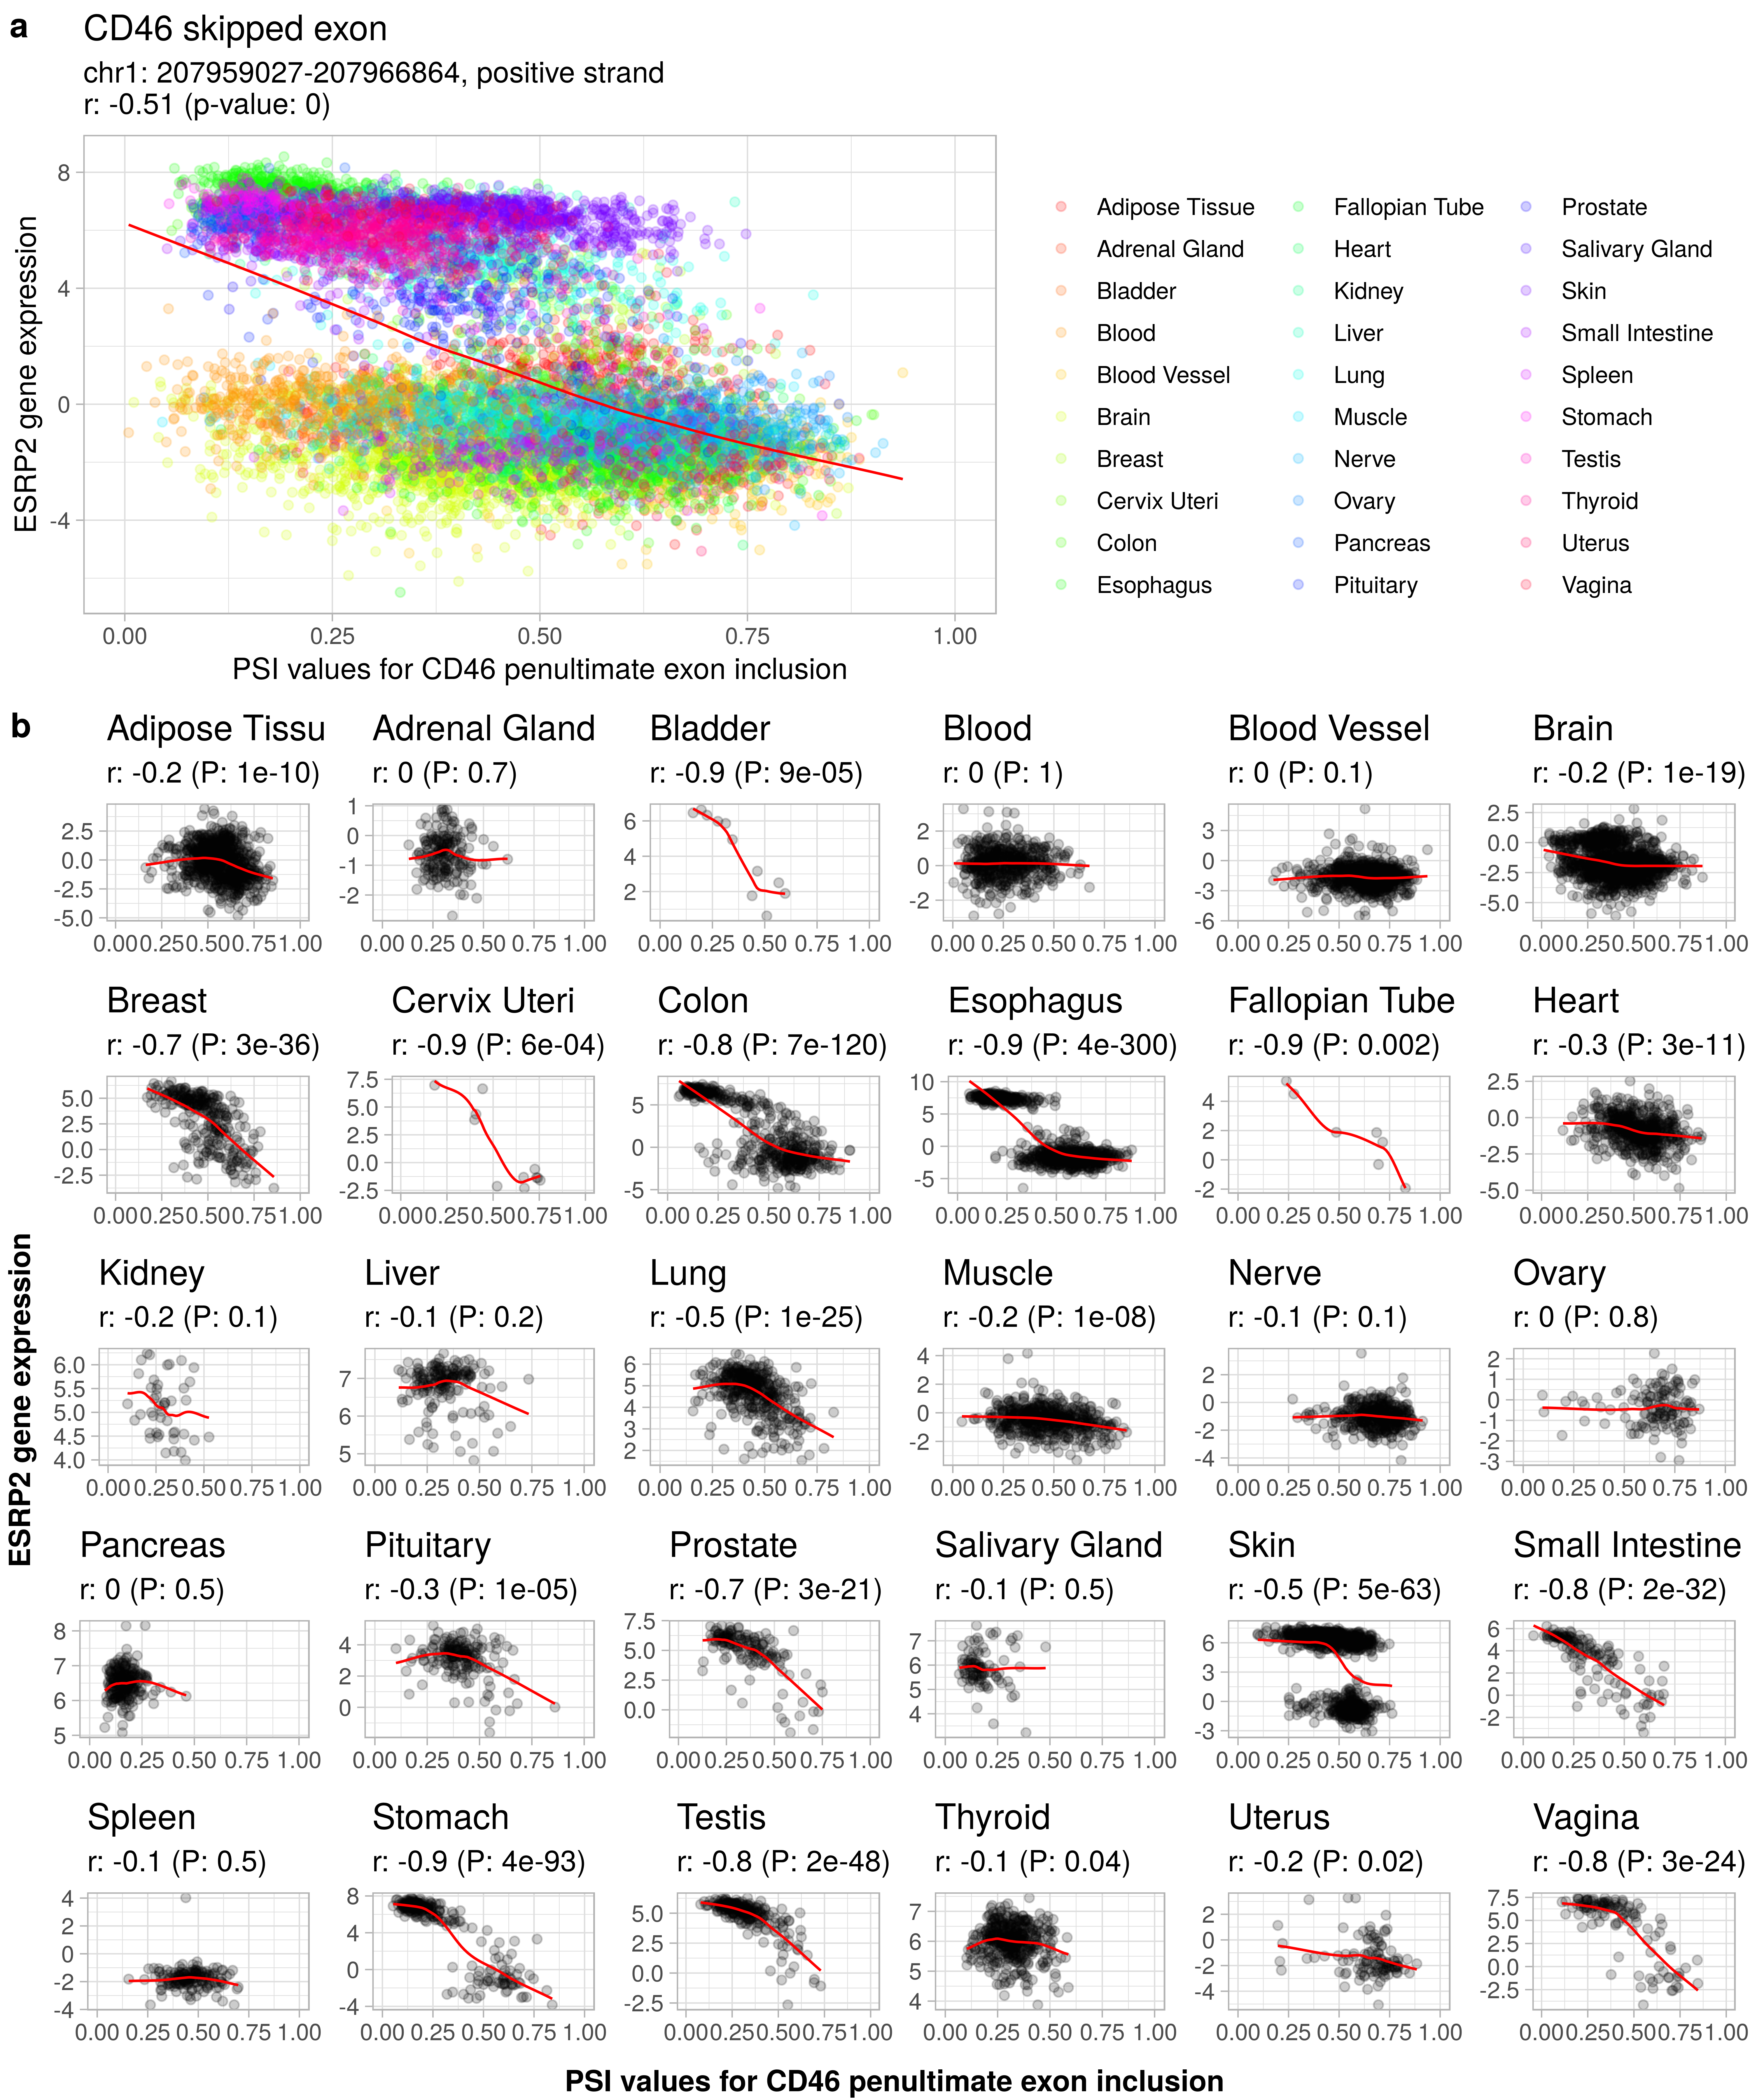
\includegraphics[width=1\textwidth]{images/psichomics/8-gtex-cor}
  \centering
  \caption[\emph{ESRP2} expression versus \emph{CD46} penultimate exon PSI in GTEx]{\textbf{Scatterplots of normalised \emph{ESRP2} expression versus PSI values for \emph{CD46} penultimate exon inclusion across GTEx tissues, altogether (a) and by tissue (b).} For each plot, the red line illustrates the fitted Loess regression curve. The Pearson’s correlation coefficients (\emph{r}) and associated p-values (P) are shown.}
  \label{fig:psichomics-gtex-cor}
\end{figure}

\begin{figure}[!p]
  \includegraphics[width=1\textwidth]{images/psichomics/9-tcga-esrp1}
  \centering
  \caption[\emph{ESRP1} expression versus \emph{CD46} penultimate exon PSI in TCGA]{\textbf{Scatterplots of normalised \emph{ESRP1} expression versus PSI values for \emph{CD46} penultimate exon inclusion across TCGA tumour types.} For each plot, the red line illustrates the fitted Loess regression curve. The Pearson’s correlation coefficients (\emph{r}) and associated p-values (P) are shown.

\hspace{\textwidth}

\textsmaller{\textbf{Legend:} ACC adrenocortical carcinoma, BCLA urothelial bladder carcinoma, BRCA breast invasive carcinoma, CESC cervical squamous cell carcinoma and endocervical adenocarcinoma, CHOL cholangiocarcinoma, COAD colon adenocarcinoma, DLBC lymphoid neoplasm diffuse large B-cell lymphoma, ESCA esophageal carcinoma, GBM glioblastoma multiforme, HNSC head and neck squamous cell carcinoma, KICH kidney chromophobe, KIRC kidney renal clear cell carcinoma, KIRP kidney renal papillary cell carcinoma, LGG brain lower grade glioma, LIHC liver hepatocellular carcinoma, LUAD lung adenocarcinoma, LUSC lung squamous cell carcinoma, MESO mesothelioma, OV ovarian serous cystadenocarcinoma, PAAD pancreatic adenocarcinoma, PCPG pheochromocytoma and paraganglioma, PRAD prostate adenocarcinoma, READ rectum adenocarcinoma, SARC sarcoma, SKCM skin cutaneous melanoma, STAD stomach adenocarcinoma, TGCT testicular germ cell tumours, THCA thyroid carcinoma, THYM thymoma, UCEC uterine corpus endometrial carcinoma, UCS uterine carcinosarcoma, UVM uveal melanoma.}
}
  \label{fig:psichomics-tcga-esrp1}
\end{figure}

\begin{figure}[!ht]
  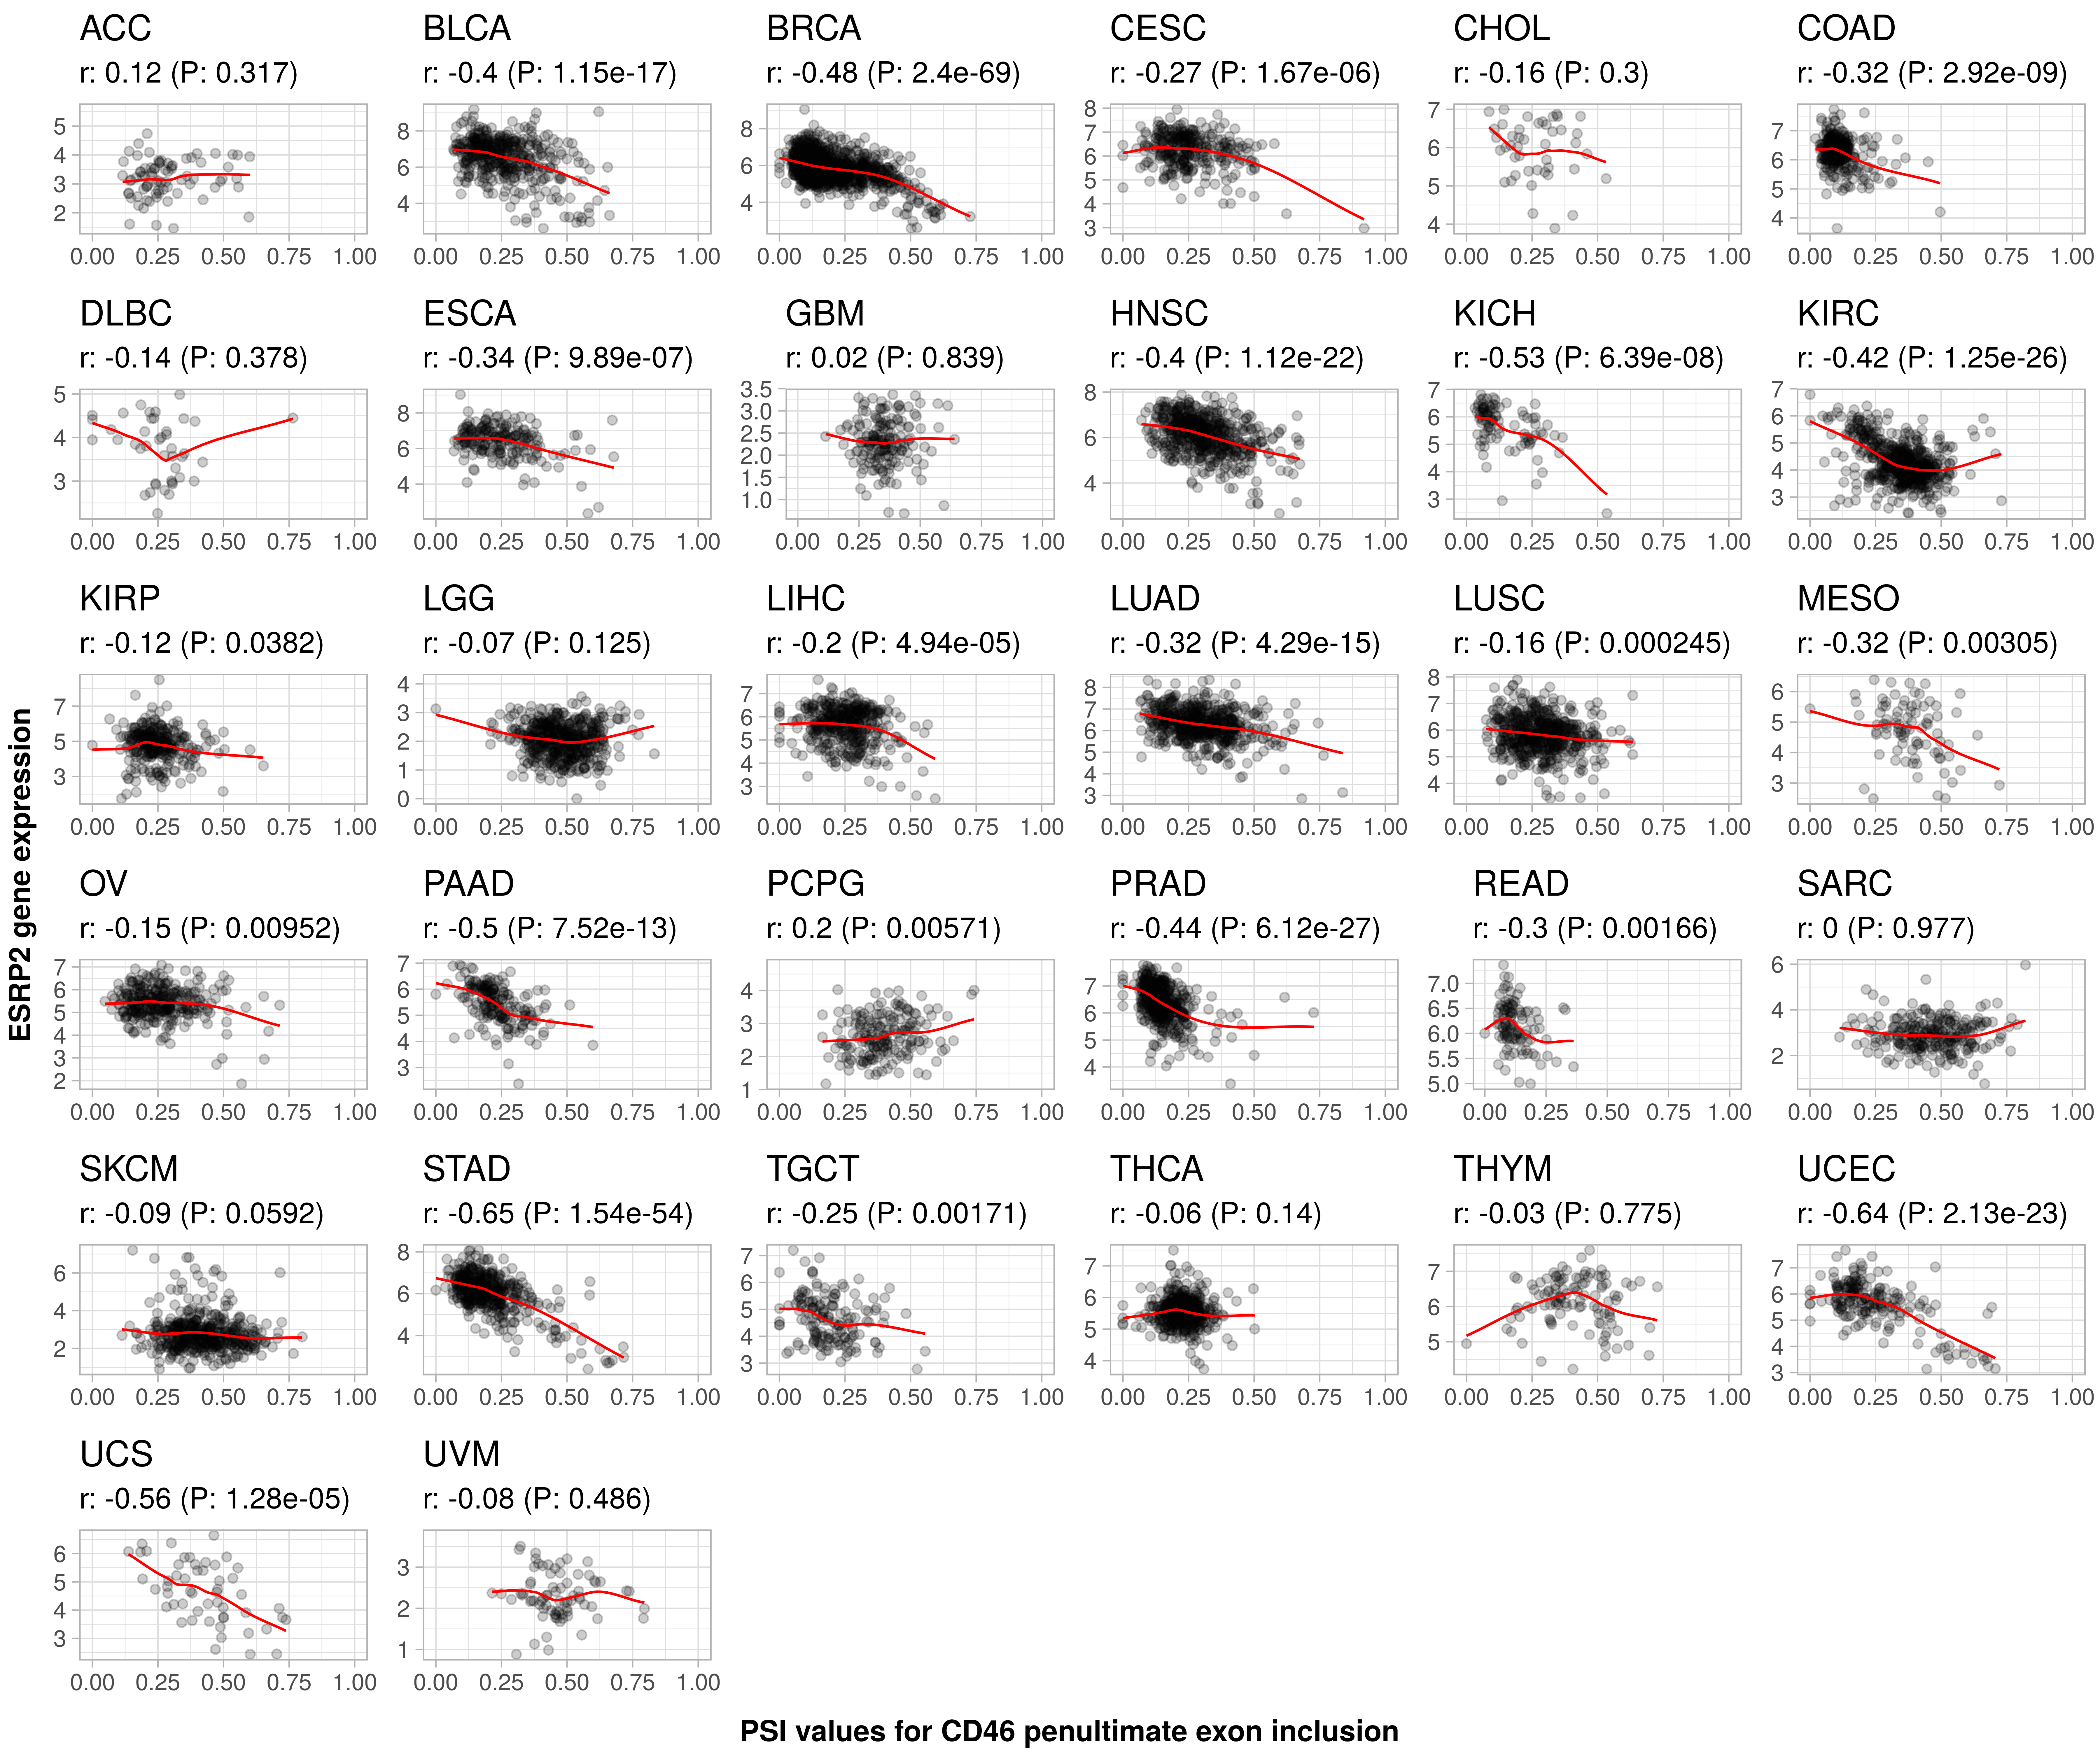
\includegraphics[width=1\textwidth]{images/psichomics/10-tcga-esrp2}
  \centering
  \caption[\emph{ESRP2} expression versus \emph{CD46} penultimate exon PSI in TCGA]{\textbf{Scatterplots of normalised \emph{ESRP2} expression versus PSI values for \emph{CD46} penultimate exon inclusion across TCGA tumour types.} For each plot, the red line illustrates the fitted Loess regression curve. The Pearson’s correlation coefficients (\emph{r}) and associated p-values (P) are shown. See caption of \shortref{fig:psichomics-tcga-esrp1} for legend.}
  \label{fig:psichomics-tcga-esrp2}
\end{figure}

\subsubsection{Pancancer prognostic value of the skipping of \emph{CD46} penultimate exon}

The prognostic value of a given alternative splicing event (or gene) may be evaluated by separating subjects based on a PSI cutoff for a given alternative splicing event (or expression cutoff for a given gene). The survival differences are then log-rank tested based on Kaplan-Meier estimators.

We performed overall survival analysis by selecting right data censoring\footnote{psichomics supports left, right, and interval data censoring for survival analysis. Events may occur after the last observation (right censoring, such as in the case of subjects having no event reported during the study or dropping from it altogether), before an observation is performed (left censoring, for instance when events happened in an uncertain time before the start of the study) or in-between observations (interval censoring, such as when patients require periodic follow-ups and the time of an event occurrence falls between follow-ups but is not certain) \cite{zhang:2010wk}.}, follow-up time as days to death and the event of interest as death. Analysing days to death as the follow-up time and death as the event of interest is known as an overall survival analysis, that is, the study of the time until the subject’s death following diagnosis. For patients whose days to death are not available, the follow-up time is based on days to last follow-up (otherwise, these subjects would be discarded from the analyses)\footnote{We recommend using days to death (complemented with days to last follow-up for missing values) as follow-up time when using TCGA data. Days to last follow-up are sometimes lower or completely missing relative to days of death, which would result in discarding individuals from the analysis.}.
 
In this context, we used clinical and transcriptomic data from TCGA to evaluate the prognostic value of the skipping of \emph{CD46} penultimate exon based on overall survival curves across TCGA tumour types to compare tumour samples with low and high inclusion of the \emph{CD46} penultimate exon. A $-log_{10}(\textrm{p-value})$ plot by cutoff displays the p-values of the log-rank test of survival across multiple PSI cutoffs for the selected alternative splicing event. The PSI cutoff maximising the significance of the survival difference is automatically selected. The splicing of \emph{CD46} penultimate exon seems to have prognostic value in select cancer types, such as brain lower-grade glioma and lung adenocarcinoma (\shortref{fig:psichomics-cd46-as-prognosis}).

% \footnote{If the PSI cutoff suggested by psichomics has unbalanced number of subjects between groups (e.g., in \shortref[d]{fig:psichomics-cd46-as}, the lowest log-rank p-value corresponds to a comparison of 1 versus 506 subjects), we should use another cutoff with more reasonably balanced groups and for which the p-value is still significant. Sample size calculations can be performed based on test assumptions (e.g., probability of failure for each group during the study) using existing R packages, such as \emph{powerSurvEpi} \cite{qiu:2021wd}.}

\begin{figure}[!ht]
  \begin{overpic}[abs,width=.8\textwidth]{images/psichomics/11-cd46-as-prognosis}
    	\put(5,175){\colorbox{white}{\textsf{\textbf{a}}}}
		\put(185,175){\colorbox{white}{\textsf{\textbf{b}}}}
	  	\put(5,35){\colorbox{white}{\textsf{\textbf{c}}}}
		\put(185,35){\colorbox{white}{\textsf{\textbf{d}}}}
  \end{overpic}
  \centering
  \caption[Prognostic value of \emph{CD46} penultimate exon inclusion]{\textbf{Prognostic value of \emph{CD46} penultimate exon inclusion across select TCGA cancer types.} (a, b) Kaplan-Meier plots of overall survival for all patients stratified by the respective alternative splicing event’s PSI cutoff that maximised the significance of differences in survival between patient groups with a reasonable number of subjects within each group. Each patient was assigned the PSI value of their tumour sample(s). (c, d) Log-rank’s $-log_{10}(\textrm{p-value})$ plot by PSI cutoff. Note that in panel d, for PSI values around 0.8, there are high log-rank $-log_{10}(\textrm{p-value})$ although only one individual is being compared against 506 subjects. Legend: LGG brain lower grade glioma, LUAD lung adenocarcinoma.}
  \label{fig:psichomics-cd46-as-prognosis}
\end{figure}

\subsection{Time benchmarking}

The runtimes required to load, quantify and analyse data from different TCGA (data version \texttt{2016\_01\_28} from FireBrowse) and GTEx v7 cohorts were benchmarked. The breast cancer cohort contains the highest number of RNA-seq samples in TCGA, thus being the cohort for which takes more time to load, quantify and analyse alternative splicing and gene expression data. Contrastingly, processed data from GTEx come bundled in files containing all tissues. Although only data from specified tissues are loaded, scanning though the large GTEx file still delays data loading. Tissues from GTEx were loaded in pairs for subsequent differential splicing analyses (\shortref[A]{fig:psichomics-performance}).

\begin{figure}[!ht]
  \begin{overpic}[abs,width=\textwidth]{images/psichomics/performance-benchmark}
  	\put(0,148){\colorbox{white}{\textsf{\textbf{a}}}}
  	\put(220,148){\colorbox{white}{\textsf{\textbf{b}}}}
  \end{overpic}
  \centering
  \caption[Performance benchmark for alternative splicing analysis]{\textbf{Performance benchmark for alternative splicing analysis using RNA-seq data from multiple TCGA and GTEx sample types.} (a) Median times of 10 runs of data loading, gene expression (GE) normalisation, skipped exon (SE) event quantification and differential expression and splicing analysis (normal versus tumour for TCGA data or pairwise tissue comparison for GTEx data) using psichomics. The default settings were used during the runs. (b) Estimation of the time complexity of each of the aforementioned steps in psichomics. Randomly generated synthetic datasets of different sample size s were used as input. Equations and coefficient of determination ($R^2$) for the best fits are displayed.}
  \label{fig:psichomics-performance}
\end{figure}

Synthetic datasets for gene expression and exon-exon junction quantification of multiple sample sizes were generated, based on TCGA data distributions, to determine the time complexity of each step in psichomics as a function of the number of input samples $s$ (\shortref[B]{fig:psichomics-performance}). Assuming a constant number of genes (20 000 in the benchmark) or exon-exon junctions (200 000), the time taken to load data grows quadratically with $s$. Gene expression normalisation and differential expression are based on commonly-used, time-efficient bioinformatics tools and the times taken for each also grow quadratically with $s$. Alternative splicing quantification is associated with element-wise operations on matrices of dimensions $s$ by the number of alternative splicing events and takes a runtime approximately proportional to the square of $s$, for a given number of alternative splicing events (around 9000 for each benchmarked run). Finally, differential splicing is based on multiple, distinct statistical analyses of alternative splicing quantification data and grows linearly with $s$.

\subsection{Alternative splicing quantification benchmarking}

Although jSplice's \cite{christinat:2016ui} and DIEGO’s \cite{doose:2018uv} splicing quantifications rely on junction read counts, their alternative splicing module expression and junction usage metrics, respectively, are not directly comparable with psichomics’ PSI values. To evaluate their accuracy in the absence of any known tool with the same input (junction read counts) and output metric (PSI) as psichomics, psichomics-estimated PSI values were compared to those estimated by RT-PCR and using VAST-TOOLS \cite{irimia:2014wt} across multiple tissue and cell line samples from human, mouse and chicken \cite{tapial:2017ui}. VAST-TOOLS follows an analogous, and therefore more directly comparable, procedure for computing PSI values and there is a substantial overlap between the alternative splicing event annotations used by the two tools. psichomics estimates highly correlate with both others, particularly for mouse and human (\shortref{fig:psi-comparison}), suggesting robustness and reproducibility in alternative splicing quantification by psichomics. Of note, the lower correlation for chicken samples is attributable to a single outlier, as its removal increases the correlation coefficients between psichomics and RT-PCR estimates (Pearson's \emph{r} = 0.87, p-value $< 0.01$; Spearman's \emph{rho} = 0.87, p-value $< 0.01$) and psichomics and VAST-TOOLS estimates (Pearson's \emph{r} = 0.93, p-value $< 0.01$; Spearman's \emph{rho} = 0.94, p-value $< 0.01$).

\begin{figure}[!ht]
  \begin{overpic}[abs,width=\textwidth]{images/psichomics/psi-comparison}
  	\put(0,157){\colorbox{white}{ }}
  	\put(146,157){\colorbox{white}{ }}
  	\put(296,157){\colorbox{white}{ }}
  \end{overpic}
  \centering
  \caption[Comparison between PSI values estimated by psichomics, VAST-TOOLS and RT-PCR]{\textbf{Comparison between PSI values estimated by psichomics, VAST-TOOLS and RT-PCR} across multiple tissue and cell line samples from human, mouse and chicken. Pearson’s (\emph{r}) and Spearman’s (\emph{rho}) correlation coefficients and respective p-values are shown. Linear regression lines are coloured per species with the respective 95\% confidence interval represented as their shades. Identity line in orange.}
  \label{fig:psi-comparison}
\end{figure}

To assess the influence of RNA-seq read coverage on psichomics PSI estimates, different numbers of junction reads per event were simulated for different given PSI values (10 000 times for each combination). \shortref{fig:psichomics-accuracy} shows that the accuracy of PSI estimation by psichomics is expectedly sensitive to junction read coverage, particularly for intermediate PSI values, with 90\% prediction intervals $<0.1$ for coverage higher than a few hundred reads.

\begin{figure}[!ht]
  \begin{overpic}[abs,width=\textwidth]{images/psichomics/psichomics-accuracy}
      	\put(-5,237){\colorbox{white}{\textsf{\textbf{a}}}}
	  	\put(219,237){\colorbox{white}{\textsf{\textbf{b}}}}
		\put(-5,115){\colorbox{white}{\textsf{\textbf{c}}}}
		\put(219,115){\colorbox{white}{\textsf{\textbf{d}}}}
  \end{overpic}
  \centering
  \caption[Event read coverage on accuracy of psichomics PSI quantification]{\textbf{Dependence of accuracy of psichomics PSI quantification on event read coverage.} (a) Comparison between simulated "real" PSI values and the mean, 95th percentile and 5th percentile of their corresponding PSI estimates for different simulated numbers of junction reads. (b) 90\% prediction interval (i.e., difference between the 95th and the 5th percentiles) across different number of junction reads for simulated "real" PSI values. (c,d) Density plots of PSI estimates for each simulated "real" PSI and junction read coverage combination (except those involving PSI $= 0$ and PSI $= 1$). Each "real" PSI and junction read coverage combination was simulated 10 000 times.}
  \label{fig:psichomics-accuracy}
\end{figure}


Alternative splicing events annotated by TCGASpliceSeq \cite{ryan:2016tm}, an online tool that displays pre-computed PSI values across multiple TCGA tumour types, were matched to those from psichomics based on their genomic coordinates. In total, 321 183 of 757 749 (42\%) skipped exon, 70 837 of 126 725 (56\%) alternative 5$'$ splice site and 90 940 of 155 799 (58\%) alternative 3$'$ splice site events were successfully matched. When available from both programs, PSI estimates for each of the 482 960 alternative splicing events in each of the 9 913 matched samples were compared between TCGASpliceSeq and psichomics, being highly correlated (N = 92 444 302; Pearson's \emph{r} = 0.97, p-value $< 10^{15}$; Spearman's \emph{rho} = 0.94, p-value $< 10^{15}$; \shortref{fig:tcgaspliceseq-correlation}).

\begin{figure}[!ht]
  \includegraphics[width=1\textwidth]{images/psichomics/tcgaspliceseq-correlation}
  \centering
  \caption[Correlation of PSI estimates between TCGASpliceSeq and psichomics]{\textbf{Correlation of PSI estimates for TCGA samples between TCGASpliceSeq and psichomics.} For A3SS events, PSI values from psichomics correspond to $1 – \textrm{PSI}$ from TCGASpliceSeq (the splice site deemed as alternative in A3SS events by TCGASpliceSeq is constitutive in psichomics and vice-versa). Pearson’s (\emph{r}) and Spearman’s (\emph{rho}) correlation coefficients and respective p-values are shown. Identity line in red.}
  \label{fig:tcgaspliceseq-correlation}
  \vspace{-\intextsep}
\end{figure}

%\subsection{Impact}

%There are multiple ways to measure the impact of psichomics. First, we can check the metrics surrounding the article itself. 

% importance of maintaining software and replying to user feedback

%- Invitation to write a book chapter

%Although there is no direct way to measure user engagement with psichomics, we can track:

%- Bioconductor downloads

%- Docker Hub image downloads 

%- visitors to the official psichomics documentation

%- visitors to the website

%- feedback via GitHub issues and emails

%- citations

%It is wonderful to see that the work I put into psichomics is appreciated based on feedback received via GitHub and email. psichomics is still used nowadays based on citations from recent published articles (Ling et al., 2020; Baeza-Centurion et al., 2020; Birladeanu et al., 2021). In the lab, we can also track visitors of psichomics’ documentation via Google Analytics to better understand our users (e.g., what pages they visit the most).

\section{Conclusion}

Alternative splicing is a regulated molecular mechanism involved in multiple cellular processes and its dysregulation has been associated with diverse pathologies \cite{kelemen:2013tc,paronetto:2016vw,wang:2008wa,oltean:2014vm}. The advent of next-generation sequencing technologies has allowed the investigation of transcriptomes of human biological samples to be expanded to alternative splicing. RNA-seq data, like those yielded by the GTEx and TCGA projects, are indeed playing crucial role in the improvement of our insights into the role of alternative splicing in both physiological and pathological contexts \cite{paronetto:2016vw,wang:2008wa,gallego-paez:2017wc,tsai:2015ve,danan-gotthold:2015ut}).

However, the most commonly used tools for alternative splicing analyses currently do not allow researchers to fully benefit from the wealth of pre-processed RNA-seq data made publicly available by the aforementioned projects. For instance, they lack support for estimating PSIs based on splice junction read counts. Such functionality would allow users to overcome the difficulties caused by the raw RNA-seq data from GTEx and TCGA being under controlled access and, more importantly, their processing requiring computational resources inaccessible to the majority of research labs. psichomics thus exploits pre-processed alternative splicing annotation and exon–exon junction read count data from TCGA and GTEx, two of the richest sources of molecular information on human tissues in physiological and pathological conditions, as well as recount2 and user-owned data, allowing researchers to hasten alternative splicing quantification and subsequent analyses by avoiding the time-consuming alignment of RNA-seq data to a genome or transcriptome of reference followed by splice junction detection.

Together with support for the integration of molecular and sample-associated clinical information, the group creation functionalities featured in psichomics ensure full customisability of data grouping for downstream analyses. Interesting groups to compare in TCGA, for instance, may range from the simple contrast between reformed and current smokers in lung cancer to complex combinations of gender, race, age, country and other subject attributes across multiple cancers. When survival data are available, survival analyses can be performed on samples by PSI or gene expression levels, thereby assessing the putative prognostic value of a respective molecular feature.

%\textcolor{red}{The integrative analysis of publicly available TCGA data by psichomics allowed us to identify multiple exons differentially spliced between breast tumour stage I and normal samples, therefore deeming them potential diagnostic biomarkers, and to assess their putative prognostic value. The output of psichomics is validated by identified alternative splicing alterations that have been previously linked to the disease, including events in RPS24, NUMB, FBLN2 and AP2B1. Previously understudied, yet intriguing, events were also identified, such as the skipping of SLMAP exon 23 and UHRF2 exon 10. These may provide novel insights into the early stages of breast cancer development.} Indeed, it is of utmost importance to foster alternative splicing analyses of clinical samples as a crucial complement to more conventional research focused on total gene expression.

To ensure researchers with different skills can take the most out of psichomics, we added an intuitive and more accessible graphical interface, while still supporting a command-line interface. psichomics has recently been deployed online at \alink{compbio.imm.medicina.ulisboa.pt/psichomics}\footnote{More information in \fullref{chap:app-server}.} to allow the on-demand use of the latest version of psichomics with no installation required, levering the intuitive graphical interface to make alternative splicing analyses more enticing to less computationally-inclined biomedical researchers.

Notwithstanding its merits, psichomics only quantifies alternative splicing events based on exon–exon junction read counts, limiting the types of alternative splicing events profiled. For instance, exon–intron junction, exon body and intron body quantifications are vital to confirm intron retention and alternative 5$'$ and 3$'$ UTR events over further transcriptional variations \cite{braunschweig:2014tr}.
However, although GTEx (but neither TCGA nor recount2) readily provides intron and exon body read quantification for retrieval, none provides exon–intron junction quantification. To overcome this, psichomics allows to import alternative splicing events quantified from other programs, including VAST-TOOLS that quantifies intron retention events.

Another limitation is psichomics' reliance on existing alternative splicing event annotations and an on the pre-processing of RNA-seq data by third-party pipelines (as is the case for GTEx, TCGA and recount2), depriving the user of the flexibility to identify \emph{de novo} alternative splicing events. Even so, when FASTQ or BAM files are accessible, psichomics supports the loading of alternative splicing annotations generated by different programs that take those files as input, namely rMATS \cite{shen:2014tk}, which is able to generate \emph{de novo} annotations\footnote{More information in \alink{nuno-agostinho.github.io/psichomics/articles/AS_events_preparation}.}.

% \textcolor{red}{Using psichomics, we are able not only to identify novel exons differentially spliced between tumour stage I and normal breast samples but also to pinpoint potentially clinically relevant splicing events by embracing clinical data and evaluating their prognostic value.}
% For future iterations of psichomics, potentially support recount3?

Since its publication, psichomics has been used to analyse alternative splicing in multiple scientific articles, such as \cite{coomer:2019wz,baeza-centurion:2019tb,munkley:2019wr,baeza-centurion:2020vb}. Based on these citations and positive user feedback, we believe that fellow researchers and clinicians are able to intuitively employ psichomics to assist them in uncovering novel splicing-associated prognostic factors and therapeutic targets, as well as in advancing our understanding of how alternative splicing is regulated in physiological and disease contexts.

% !TEX root = ../PhD Thesis.tex

%\chapter{cTRAP: identification of candidate causal perturbations from differential gene expression data}
\chapter{cTRAP}
\label{chap:ctrap}

\begin{figure}[!b]
  \vspace*{-1cm}
  \includegraphics[width=.96\textwidth]{images/cTRAP/screenshot}
  \centering
  \vspace*{-.5cm}
  \caption[cTRAP global interface screenshot]{\textbf{cTRAP global interface screenshot} (21 Dec 2021).}
  \label{fig:cTRAP-screenshot}
\end{figure}

During a stormy day in our 2017 Madeira Lab retreat, we brainstormed the unique propositions of the lab that could most benefit the scientific community. One idea that emerged was to make it easier to identify putative causal perturbations by comparing the results of a custom differential gene expression analysis against the large-scale database of differential expression profiles from CMap \cite{subramanian:2017ul}, a repository of transcriptomic signatures for thousands of genetic (gene overexpression or knockout) and pharmacological perturbations of human cancer cell lines. % This kind of analysis is available in CMap's web apps at \alink{clue.io} \cite{subramanian:2017ul}, but their results are difficult to integrate in downstream analyses, suffer from poor API documentation for programatic access and lack basic visualisation tools.

% clue.io does indeed allow for batch query: https://clue.io/connectopedia/batch_query_tutorial
% clue.io API's is not straightforward: https://clue.io/connectopedia/query_api_tutorial

We thus developed cTRAP, an R package and web app to compare user-provided differential gene expression profiles with the perturbations available from CMap, allowing to infer putative candidate molecular causes for the observed differences, as well as compounds that may promote or revert them (\shortref{fig:cTRAP-screenshot}).

After releasing the first version in Bioconductor, multiple features were added (\shortref{tab:cTRAP}). Inspired by the method used to compare gene expression changes against the CMap database, we also added a way to predict drugs targeting altered genes by using datasets that featured both drug sensitivity and gene expression data for many cell lines. Additionally, cTRAP also allows to analyse the enrichment of molecular descriptor sets for compounds from NCI-60 and CMap. More recently, we developed a Shiny-based visual interface to host cTRAP online with support for user sessions and background tasks.

\begin{table}[!ht]
\parnotereset
\small
\caption[Major cTRAP milestones]{\textbf{Major cTRAP milestones.}}
\label{tab:cTRAP}
\begin{tabularx}{\textwidth}{ l r l }
\toprule
\textbf{Version} & \textbf{Release date} & \textbf{Main features} \\
\midrule
1.0  &  2 Nov 2018 & Compare differential expression profiles against CMap data\parnote{First Bioconductor release.} \\
\midrule
\multirow{3}*{1.4}  & \multirow{3}*{12 Nov 2019} & Predict targeting drugs using NCI-60, CTRP and GDSC data \\
       &             & Analyse enrichment for molecular descriptors of compounds \\
       &             & Load and process 21GB CMap z-scores file by chunks \\
\midrule
1.8  & 30 Oct 2020 & Include graphical functions to load data and analyse results \\
\midrule
\multirow{2}*{1.10} & \multirow{2}*{20 May 2021} & Improve speed and memory usage when comparing data \\
       &             & Set custom size for data chunks (1 GiB by default)  \\
\midrule
1.12 & 28 Oct 2021 & Add web server support (optimised to run in ShinyProxy)\parnote{First version available online.} \\
\bottomrule
\end{tabularx}
\parnotes
\end{table}

The associated cTRAP manuscript (of which I am a co-first and co-corresponding author) is in preparation for submission to an international peer-reviewed scientific journal and shares similarities with this chapter.

\section{Background}

Understanding the biological mechanisms underlying uncharacterised phenotypes is crucial to unravel the physiological role of genes and the mechanism of action of compounds, alongside their therapeutic potential \cite{subramanian:2017ul,malta:2018uj,mendez-lucio:2020th,le:2021uq,hughes:2000ww,almeida:2019wh}. Comprehending novel genetic and pharmacological perturbations -- including the modulation of the expression of a gene or induction of an unknown compound in a cellular system -- can be achieved by profiling genome-wide gene expression, allowing to analyse the whole cellular transcriptional response \cite{hughes:2000ww}.
% based on the assumption that cellular transcriptional response to pathway disruption is similar across cells, and that there are sufficiently unique transcriptional responses to the perturbation of most cellular pathways, systematic characterization of novel mutants could be carried out with a single genome-wide expression measurement

The gene expression profile of experimental phenotypic changes can be compared with a database of characterised transcriptomic signatures of known perturbagens, in order to infer putative molecular causes of the observed phenotype \cite{subramanian:2017ul,hughes:2000ww}. This approach requires a large, heterogeneous and representative dataset containing gene expression profiles associated with known perturbagens across multiple cell lines \cite{hughes:2000ww}. Such is the case of the Connectivity Map (CMap), a repository of transcriptomic signatures of thousands of genetic and pharmacological perturbations of human cancer cell lines \cite{subramanian:2017ul}. %Comparing differential gene expression profiles with those from CMap allows to infer putative molecular causes for the observed differences, as well as compounds that may promote or revert those changes.

CMap data can be explored and compared with user-provided data via a collection of user-friendly web apps from the CMap and LINCS Unified Environment (\mbox{\alink{clue.io}}) \cite{subramanian:2017ul}. However, \alink{clue.io} limits the maximum number of input genes for CMap queries (150 up-regulated and 150 down-regulated genes), %expresses results' significance in a non-standard significance score,
is difficult to automate for downstream analyses and cannot be run using local computing resources. Furthermore, \alink{clue.io} does not currently integrate with drug sensitivity datasets to further assist in pinpointing compounds that selectively target cells \cite{almeida:2019wh}.

\begin{figure}[!b]
  \includegraphics[width=\textwidth]{images/ctrap/ctrap}
  \centering
  \caption[cTRAP analyses]{\textbf{cTRAP analyses.} cTRAP allows to perform three types of analyses: \textbf{(1) rank CMap perturbations} based on the similarity between their associated gene expression alterations and user-provided differential gene expression values, \textbf{(2) predict targeting drugs} by comparing user-provided differential gene expression values with matrices of correlation between gene expression and drug sensitivity data across human cell lines and \textbf{(3) analyse drug descriptor set enrichment} (v. main text) using the compound list from either the first or second analysis.}
  \label{fig:ctrap}
\end{figure}

We thus developed cTRAP (\shortref{fig:ctrap}), an R package and web app that identifies potentially causal molecular perturbations by seamlessly comparing user-provided differential gene expression results with those available from CMap. cTRAP also supports comparisons with gene expression/drug sensitivity associations derived from the NCI-60 \cite{shoemaker:2006wi}, the Cancer Therapeutics Response Portal (CTRP) \cite{seashore-ludlow:2015ws} and the Genomics of Drug Sensitivity in Cancer (GDSC) \cite{yang:2012vk}, to identify compounds that could target the phenotypes associated with the user-provided differential expression profiles \cite{almeida:2019wh}. In cTRAP, similarity between differential gene expression results is measured by gene set enrichment \cite{subramanian:2017ul,subramanian:2005wu} and correlation scores. Finally, cTRAP can also analyse a list of compounds resulting from previous analyses for the enrichment in sets of computed molecular descriptors (e.g., number of oxygen atoms or aromatic rings) from CMap and NCI-60 compounds, allowing to identify common chemical properties of compounds of interest.

cTRAP is available online as a web app at \alink{compbio.imm.medicina.ulisboa.pt/cTRAP}, but can be locally installed using Bioconductor (\alink{bioconductor.org/packages/cTRAP}) or Docker (\dockerlink{nunoagostinho/ctrap}). The source code of cTRAP is available at \alink{github.com/nuno-agostinho/cTRAP}.

\section{Materials and methods}

From a vector of user-provided differential expression results (e.g., t-statistic values) with respective gene symbols, cTRAP can return a list of CMap perturbations ranked by similarity or predict candidate drugs for targeting the associated phenotype. Moreover, cTRAP can also analyse the enrichment of drug sets in an ordered vector of compounds to identify common chemical characteristics (Figures \shorterref{fig:ctrap-workflow} and \shorterref{fig:ctrap-file-structure}).

\begin{figure}[!ht]
  \includegraphics[width=.8\textwidth]{images/ctrap/workflow}
  \centering
  \caption[cTRAP workflow]{\textbf{cTRAP workflow.} A vector of differential gene expression values containing gene names is required to rank similar perturbations and to predict targeting drugs. Drug descriptor set enrichment analysis can then be performed based on those results. CMap perturbagen data, gene expression/drug sensitivity correlation matrices and molecular descriptors for drug sets can be automatically downloaded by cTRAP.}
  \label{fig:ctrap-workflow}
\end{figure}

\begin{figure}[!ht]
  \includegraphics[width=1\textwidth]{images/ctrap/file-structure}
  \centering
  \caption[cTRAP file structure]{\textbf{Visual representation of cTRAP's file structure.} As usual in an R package, the \texttt{R} folder contains the scripts with cTRAP functions and data. \texttt{dev} is a custom folder that stores supporting scripts (e.g., test workflows and benchmarks); its contents are not included when building the R package.}
  \label{fig:ctrap-file-structure}
\end{figure}

\subsection{ENCODE knockdown data}

Using cTRAP, we can query and download ENCODE knockdown (and respective control) samples \cite{luo:2019tp} for multiple cell lines, filter genes/samples with low coverage from gene expression data, convert from ENSEMBL gene identifiers to gene symbols, and perform differential gene expression analysis using \texttt{voom()}, \texttt{lmFit()} and \texttt{eBayes()} from the \texttt{limma} R package \cite{ritchie:2015tm}. First, \texttt{voom()} is used with the \emph{quantile} normalisation to transform count data to log\textsubscript{2} CPM (counts per million) and estimate the mean-variance relationship to compute weights used in linear modelling. Gene-wise linear models are then fitted using \texttt{lmFit()} between the knockdown and the control samples, followed by moderated t-tests and the calculation of log-odds of differential expression, using \texttt{eBayes()} for empirical Bayes moderation of standard errors.

cTRAP includes an example dataset (\texttt{diffExprStat}) with the differential gene expression results (t-statistic values) associated with \emph{EIF4G1} knockdown in HepG2 cells (\shortref{lst:diffExprStat}).

\begin{lstlisting}[caption=Code to obtain example dataset \texttt{diffExprStat}.,language=R,label={lst:diffExprStat}]
library(cTRAP)
ENCODEmetadata <- downloadENCODEknockdownMetadata(cellLine="HepG2",
                                                  gene="EIF4G1")
ENCODEsamples  <- loadENCODEsamples(ENCODEmetadata)[[1]]
counts         <- prepareENCODEgeneExpression(ENCODEsamples)

# Remove low coverage genes (>= 10 counts shared by >= 2 samples)
minReads   <- 10
minSamples <- 2
filter     <- rowSums(counts[ , -c(1, 2)] >= minReads) >= minSamples
counts     <- counts[filter, ]

# Convert ENSEMBL identifiers to gene symbols
counts$gene_id <- convertGeneIdentifiers(counts$gene_id)

# Perform differential gene expression (DGE) analysis
diffExpr <- performDifferentialExpression(counts)

# Get t-statistic values of DGE and respective gene names
diffExprStat <- diffExpr$t
names(diffExprStat) <- diffExpr$Gene_symbol
\end{lstlisting}

\subsection{Ranking of similar CMap perturbations}

\begin{figure}[!b]
  \includegraphics[width=.8\textwidth]{images/ctrap/cmap-perturbations}
  \centering
  \caption[Loading data from CMap perturbations]{\textbf{Loading data from CMap perturbations.} Input arguments support either the data themselves (as data frames) or their respective file path. If the file path directs to a non-existing file,  data are first downloaded and then saved to the given file path. To avoid high memory usage, CMap perturbations' differential expression z-scores (CMap zscores) are not loaded into memory when a file path is given. Instead, only metadata are loaded into a \emph{dummy} object that can be subset as a normal R object for downstream analyses.}
  \label{fig:ctrap-cmap-perturbations}
\end{figure}

CMap perturbations can be categorised into gene knockdown, gene over-expression and compounds. In cTRAP, available perturbation types and respective conditions can be enquired using the function \texttt{getCMapConditions()} that will download CMap perturbation metadata. Afterwards, \texttt{filterCMapMetadata()} allows to filter the metadata based on selected perturbations types, cell lines, dosages and time points, allowing to specifically load only the desired data in downstream analyses. This information is passed to \texttt{prepareCMapPerturbations()} to download (if file is not found) and process CMap differential expression normalised z-scores (GCTX file) and gene and compound information (\shortref{fig:ctrap-cmap-perturbations}). Given that the GCTX file size is around 21GB, we recommend to download the file directly from GEO GSE92742’s Level 5 data link (\sloppy{\small{\url{ftp://ftp.ncbi.nlm.nih.gov/geo/series/GSE92nnn/GSE92742/suppl/GSE92742_Broad_LINCS_Level5_COMPZ.MODZ_n473647x12328.gctx.gz}}}).

After comparing differential expression normalised z-scores from select CMap perturbations against user-provided differential expression results, \texttt{rankSimilarPerturbations()} returns a table with ranked CMap perturbations. Ranks closer to the top indicate perturbations whose differential expression profiles are more similar to the user-provided data, i.e., CMap perturbations that potentially mimic the user-provided transcriptomic changes, whereas higher ranks define perturbations that may revert those changes.

To rank CMap perturbations, cTRAP performs Spearman's and Pearson's correlations between the user-provided statistics for differential expression and values from CMap perturbations, and calculates a GSEA-based score (described below). All three methods are run by default. For each method, the similarity scores are averaged across multiple cell lines for the same conditions (i.e., same exposure time, dose and induced compound or gene target) and those averages are then used to rank CMap perturbations. By default, results for individual cell lines are provided for informative purposes (e.g., to check the heterogeneity of response across cell lines) but not used when ranking. The different ranking scores are combined via the rank product \cite{breitling:2004aa}, ultimately used to sort the CMap perturbations. % rank product not properly explained

The GSEA-based score is calculated via the following steps:

\begin{enumerate}
	\item Order genes by the user-provided differential expression statistics.
	\item Define the top 150 (by default) and bottom 150 (by default) genes as two sets.
	\item For each CMap perturbation, sort genes by their differential expression z-scores and calculate the Weighted Connectivity Score (WTCS), a composite and bi-directional version of the weighted Kolmogorov-Smirnov enrichment statistic (ES) \cite{subramanian:2017ul} where GSEA is run for the most up- and down-regulated genes from the user’s differential expression profile. The WTCS is the mean between $\textrm{ES}_{\textrm{top}}$ and $\textrm{ES}_{\textrm{bottom}}$; however, $\textrm{WTCS} = 0$ if both sets have the same sign \cite{subramanian:2017ul}.
\end{enumerate}

As an example, for a CMap perturbation with a similar differential expression profile to user’s input, we expect to find higher enrichment of the top gene set in the most up-regulated genes and higher enrichment of the bottom gene set in the most down-regulated genes.

To minimise peak RAM usage, \texttt{prepareCMapPerturbations()} downloads the GCTX file (a customised HDF5 file) for the CMap’s perturbation differential expression z-scores (if not previously downloaded) and returns its path without loading the file content itself, creating a \emph{dummy} object that only stores its file path, perturbation names, gene symbols and other associated metadata (\shortref{fig:ctrap-cmap-perturbations}). Based on the file path of this \emph{dummy} object (that can be subset like a normal R object), \texttt{rankSimilarPerturbations()} loads a $\le$ 1 GiB chunk\footnote{The default 1 GiB ($1024^3$ bytes) allows loading chunks of around 10000 columns and 14000 rows ($10000 \times 14000 \times 8 \textrm{ bytes} / 1024^3 = 1.04 \textrm{ GiB}$). CMap's GCTX file has around 14000 rows (genes).}, compares its differential expression z-score values against user-provided data and repeats the analysis for the next chunk (\shortref{fig:ctrap-analyses}). For each chunk, multithreaded support for Linux and macOS can be enabled per comparison method via \texttt{parallel::mclapply()}\footnote{\texttt{mclapply()} parallelises tasks via forking where multiple child processes are spawned and share their parent's memory. Forking is unavailable in Windows and its alternatives were deemed unsatisfactory, given that they copy 1GiB chunks per thread, significantly slowing down runtime.}, enabled by setting the number of threads to 2 or higher.

\begin{figure}[!ht]
  \includegraphics[width=.8\textwidth]{images/ctrap/analysis}
  \centering
  \caption[cTRAP similarity analysis]{\textbf{cTRAP similarity analysis.} User-provided differential gene expression statistics are compared with reference data (e.g., differential expression z-scores of CMap perturbations) and ranked by similarity. If the reference is contained in an HDF5 file, the file is processed in 1 GiB chunks (by default) to minimise peak memory usage. These analyses support multiple threads in Linux and macOS.}
  \label{fig:ctrap-analyses}
\end{figure}

The ranked list from \texttt{rankSimilarPerturbations()} can be plotted using \texttt{plot()}, showing a list of all results ordered by a given score or either a scatterplot or GSEA plot of the results for a single CMap perturbation (examples shown in \fullref{subsec:case-study}).

\pagebreak
\subsection{Prediction of targeting drugs}

Gene expression and drug activity data across multiple cell lines are available from NCI-60 \cite{shoemaker:2006wi}, Cancer Therapeutics Response Portal (CTRP) 2.1 \cite{seashore-ludlow:2015ws} and Genomics of Drug Sensitivity in Cancer (GDSC) 7 \cite{yang:2012vk} (\autoref{tab:drug-sensitivity-datasets}). For each source, the \texttt{prepareExpressionDrugSensitivityAssociation()} function performs the following:

\begin{enumerate}
	\item download all the necessary data depending on given source;
	\item perform Spearman’s correlation (by default) across cell lines between the expression of each gene and the sensitivity to each drug;
	\item generate a matrix with the correlation coefficients per gene and drug; and
	\item prepare metadata for downstream analyses, including gene, compound and cell line information from each source.
\end{enumerate}

As this process can take multiple hours to finish for all sources, the resulting objects were stored online for each aforementioned source and can be listed with \texttt{listExpressionDrugSensitivityAssociation()} and downloaded and loaded into R using \texttt{loadExpressionDrugSensitivityAssociation()}.

A positive correlation coefficient for a given gene and drug suggests a gene whose expression is associated with sensitivity to that drug across multiple cell lines. By calculating the susceptibility of genes for each annotated drug, we can then correlate this information with a given phenotype to rank compounds based on their potential to selectively target the queried (or similar) phenotypes, i.e., to selectively target phenotypes characterised by the overexpression of genes conferring susceptibility to the compounds.

\begin{wraptable}{r}{7cm}
\centering
\parnotereset
\small
\caption[Drug sensitivity datasets statistics]{\textbf{Drug sensitivity dataset statistics.} Number of screened compounds and human cancer cell lines available in cTRAP datasets.}
\label{tab:drug-sensitivity-datasets}
\begin{tabularx}{.45\textwidth}{ l r r }
\toprule
\textbf{Source}   & \textbf{Compounds} & \textbf{Cell lines} \\
\midrule
NCI-60            &             21 738 &   60 \\
GDSC 7            &                266 &  983 \\
CTRP 2.1          &                545 &  823 \\
\bottomrule
\end{tabularx}
\parnotes
\end{wraptable}

To identify compounds that could target the phenotype associated with specific differential expression profiles, we use \texttt{predictTargetingDrugs()} with those profiles and a correlation matrix of gene expression and drug sensitivity as input. The correlation coefficients between gene expression and drug sensitivity for each drug are compared against user-provided differential expression results by Spearman’s and Pearson’s correlation and WTCS (as performed when ranking CMap perturbations, results from comparison methods are ranked and then those rankings are finally used to calculate the rank product’s rank). \texttt{predictTargetingDrugs()} returns a table with ranked predicted targeting drugs and their respective correlation coefficients and WTCS (\shortref{fig:ctrap-analyses}). The ranks closer to the top comprise drugs that may target phenotypes similar to the user-provided differential expression profile.

The resulting object can be plotted with \texttt{plot()}, showing a list of all results ordered by a given score or either plots for a single predicted targeting drug. The function \texttt{plotTargetingDrugsVSsimilarPerturbations()} compares the results from predicted targeting drugs and CMap perturbations that may mimic or revert the observed phenotype. For the available compound identifiers in the metadata pertaining from the different datasets (e.g., compound name, Broad ID, PubChem CID and SMILES), the function will automatically select the identifiers with higher number of matching values between the two datasets, unless the identifiers are explicitly defined by the user. A scatterplot is then returned using, by default, the rank product’s rank of targeting drugs against the rank product’s rank of similar perturbations (examples shown in \fullref{subsec:case-study}).

\subsection{Drug descriptor set enrichment analysis}
\label{subsec:descriptor-set-enrichment}

Juan Carlos, a former member of the lab, computed drug descriptors (e.g., molecu\-lar weight and number of aromatic rings) for compounds from CMap and NCI-60 based on their three-dimensional (3D) and two-dimensional (2D) characteristics. These descriptors were uploaded to \alink{compbio.imm.medicina.ulisboa.pt/public/cTRAP/} and the resulting files can be automatically downloaded and processed to R using \texttt{loadDrugDescriptors()}.

\texttt{prepareDrugSets()} allows to create sets of descriptors. By default, the function creates a maximum of 15 sets per drug descriptor. For each alphanumeric descriptor, one set is created per unique value of that descriptor. Alphanumeric descriptors containing more than 15 unique values (by default) will be discarded. For numerical descriptors, \texttt{prepareDrugSets()} internally uses the \texttt{binr::bins()} function to create evenly-distributed bins of drug descriptors, where each set contains a minimum number of points equal to the number of non-missing values divided by the number of maximum sets (15 by default) divided by a constant (5 by default).

The \texttt{analyseDrugSetEnrichment()} function analyses the enrichment of the created drug descriptor sets in a named numeric vector or an object returned from \texttt{rankSimilarPerturbations()} or \texttt{predictTargetingDrugs()}. The GSEA-based enrichment analysis is internally performed using \texttt{fgsea::fgsea()} \cite{sergushichev:2016aa}. The resulting object can be plotted with \texttt{plot()}, showing a list of all results ordered by a given score or plots for a single predicted targeting drug.

\subsection{Time and memory benchmarking}

We measured elapsed time using R’s \texttt{Sys.time()} immediately before and after ranking similar CMap perturbations, predicting targeting drugs (using NCI-60 expression and drug sensitivity association, the most time-consuming option) and performing drug set enrichment analysis using a development version of cTRAP 1.10 (commit \link{https://github.com/nuno-agostinho/cTRAP/commit/296f9b2}{296f9b2} from January 2022). As input, we used the t-statistics for the differential expression between \emph{EIF4G1} knockdown versus control based on ENCODE gene expression data for cell line HepG2 (\texttt{cTRAP::diffExprStat} object).

Using the same input, we measured heap memory usage of cTRAP 1.10 dev (\link{https://github.com/nuno-agostinho/cTRAP/commit/296f9b2}{296f9b2}) while ranking CMap perturbations when running R 4.0.3 in debug mode with heaptrack 1.0.0\footnote{heaptrack is an open-source memory allocation profiler available at \alink{github.com/KDE/heaptrack}}. For R to work properly with heaptrack, the \path{/usr/bin/R} file was edited -- all lines of the last \emph{if} statement were commented out, except for:

\begin{lstlisting}[language=bash,numbers=none]
exec ${debugger} ${debugger_args} "${R_binary}" ${args} "${@}"
\end{lstlisting}

Afterwards, we benchmarked the memory usage while running cTRAP with:

\begin{lstlisting}[language=bash,numbers=none]
R -d heaptrack -f ${cTRAP_Rscript} --args ${cTRAP_Rscript_args}
\end{lstlisting}

All benchmarks were run in a workstation with Ubuntu 18.04.5 LTS, 768 GB of RAM memory and 72 cores (Intel Xeon Gold 6254 CPU @ 3.10GHz). The benchmark scripts are open-source and describe how to profile time and memory in cTRAP and plot subsequent results: \alink{github.com/nuno-agostinho/cTRAP/tree/master/dev/benchmark}.

\subsection{Continuous integration}

Akin to psichomics (\fullref{subsec:psichomics-ci}), GitHub Actions are used with cTRAP to update its Docker images in Docker Hub (\dockerlink{nunoagostinho/ctrap}) and GitHub (\alink{github.com/nuno-agostinho/cTRAP}); update website documentation via \texttt{roxygen} \cite{wickham:2021wt} and \texttt{pkgdown} \cite{wickham:2021wj}; and check for errors and warnins when building cTRAP in Windows, macOS and Linux.

\section{Results}

cTRAP's web app is available at \alink{compbio.imm.medicina.ulisboa.pt/cTRAP}. Alternatively, users can install cTRAP, allowing them to use local computing resources. Similarly to psichomics, cTRAP offers both graphical and command-line interfaces. Although most features are common to both interfaces, we recommend less experienced users to opt for the Shiny-based graphical interfaces.

\subsection{Case study}
\label{subsec:case-study}

To showcase cTRAP, we used RNA-seq data from \emph{EIF4G1} shRNA knockdown experiments in the HepG2 cell line from the ENCODE project \cite{luo:2019tp}. \emph{EIF4G1} (Eukaryotic Translation Initiation Factor 4 Gamma 1) encodes for the EIF4G1 scaffolding protein that contains binding sites for subunits of the EIF4F protein complex, required to initiate cap-dependent translation \cite{luo:2019tp,tu:2010vi,jaiswal:2018uq}. EIF4G1 is involved in cancer cell proliferation and migration and \emph{EIF4G1} knockdown has been suggested to impair tumourigenicity in prostate and epithelial cancer cells \cite{tu:2010vi,jaiswal:2018uq}.

Using cTRAP functions, we downloaded pre-processed gene quantification data for \emph{EIF4G1} knockdown (ENCFF955TXI and ENCFF049UZV, two replicates) and controls (ENCFF657KMW and ENCFF726AVT) from ENCODE \cite{luo:2019tp}. Afterwards, we quantilise-normalised the gene expression data with \texttt{voom} \cite{ritchie:2015tm} and performed differential expression analysis with \texttt{limma} \cite{ritchie:2015tm}.

\subsubsection{Comparison with CMap perturbations}

We compared ENCODE's t-statistic for the \emph{EIF4G1} knockdown expression changes against the normalised z-scores associated with CMap's knockdown and small molecule perturbations in HepG2\footnote{This comparison could also be performed to perturbations in a different cell line (or in all cell lines using the average result across cell lines).}. The comparisons were performed using Spearman's correlation, Pearson's correlation and WTCS (using the default 150 up-regulated and 150 down-regulated genes). All results were ordered based on the rank product's rank.

Within CMap knockdown perturbations, the top result is expectedly the knockdown of \emph{EIF4G1} in CMap data, working as a positive control (\autoref{tab:eif4g1-cmap-kd} and \autoref{fig:eif4g1-compound-plots}).

\begin{table}[!ht]
\centering
\footnotesize
\caption[Top 10 CMap HepG2 gene knockdown perturbations]{\textbf{Top 10 most similar CMap HepG2 gene knockdown perturbations} compared to \emph{EIF4G1} knockdown profile. Results ordered by rank product's rank. Legend: \emph{rho} is Spearman's coefficient and \emph{r} is Pearson's coefficient.}
\label{tab:eif4g1-cmap-kd}
\begin{tabular}{lllllllllllll}
\toprule
\textbf{Gene}     & \textbf{\emph{rho}} & \textbf{\emph{r}} & \textbf{WTCS} & \textbf{Gene description}                           \\
\midrule
\textbf{EIF4G1}   & 0.18         & 0.19       & 0.49          & eukaryotic translation initiation factor 4 gamma, 1 \\
\textbf{SKIV2L}   & 0.14         & 0.18       & 0.51          & Ski2 like RNA helicase                              \\
\textbf{MECP2}    & 0.19         & 0.18       & 0.39          & methyl-CpG binding protein 2                        \\
\textbf{KIF20A}   & 0.17         & 0.18       & 0.46          & kinesin family member 20A                           \\
\textbf{MEST}     & 0.17         & 0.19       & 0.42          & mesoderm specific transcript                        \\
\textbf{COPS5}    & 0.18         & 0.18       & 0.42          & COP9 signalosome subunit 5                          \\
\textbf{PPIH}     & 0.19         & 0.17       & 0.44          & peptidylprolyl isomerase H                          \\
\textbf{STAT1}    & 0.18         & 0.19       & 0.38          & signal transducer and activator of transcription 1  \\
\textbf{KIAA0196} & 0.19         & 0.18       & 0.35          & KIAA0196                                            \\
\textbf{SQRDL}    & 0.19         & 0.17       & 0.40          & sulfide quinone reductase-like (yeast)             \\
\bottomrule
\end{tabular}
\end{table}

\begin{figure}[!ht]
	\centering
	  \vspace{-\intextsep}
	\begin{subfigure}[h]{0.45\textwidth}
		\begin{overpic}[width=\textwidth]{images/ctrap/eif4g1-compound-plot-scatter}
			\put(1,85){\textsf{\textbf{a}}}
		\end{overpic}
	\end{subfigure}
	\begin{subfigure}[h]{0.45\textwidth}
		\begin{overpic}[abs,width=\textwidth]{images/ctrap/eif4g1-compound-plot-gsea}
			\put(.6,167){\textsf{\textbf{b}}}
			\put(.6,107){\textsf{\textbf{c}}}
			\put(.6,54){\textsf{\textbf{d}}}
		\end{overpic}
	\end{subfigure}
    \caption[Comparison of \emph{EIF4G1} knockdown in HepG2 between ENCODE and CMap]{\textbf{Comparison of the \emph{EIF4G1} knockdown experiments in HepG2 cells between ENCODE and CMap.} (a) Scatterplot of differential gene expression values of \emph{EIF4G1} knockdown for common genes between ENCODE (t-statistics; X-axis) and CMap (normalised z-scores; Y-axis). (b-d) GSEA plot of the enrichment of the most up- (b) and down-regulated (c) genes from ENCODE \emph{EIF4G1} knockdown relative to the ranked genes from the CMap perturbation (d). The genes are ranked (X-axis) based on the CMap normalised z-scores (Y-axis).}
    \label{fig:eif4g1-compound-plots}
\end{figure}

\pagebreak
Afterwards, we compared the \emph{EIF4G1} knockdown gene expression changes against those associated with CMap compound perturabtions in HepG2 (\autoref{tab:eif4g1-cmap-compounds}). The knockdown of \emph{EIF4G1}, a gene that encodes for a translation initiation factor subunit relevant in the assembly of the EIF4F complex for initiation of cap-dependent translation \cite{tu:2010vi,jaiswal:2018uq,luo:2019tp}, shows a similar expression profile to the perturbation caused by homoharringtonine, a translation elongation inhibitor.

\begin{table}[!ht]
\centering
\footnotesize
\caption[Top 10 CMap HepG2 compound perturbations]{\textbf{Top 10 most similar CMap HepG2 compound perturbations} compared to the differential expression profile of \emph{EIF4G1} knockdown in HepG2 cells from ENCODE. Results ordered by rank product's rank. Legend: \emph{rho} is Spearman's coefficient, \emph{r} is Pearson's coefficient and Time is the exposure time.}
\label{tab:eif4g1-cmap-compounds}
\begin{tabular}{llllllll}
\toprule
\textbf{Compound}     & \textbf{\emph{rho}} & \textbf{\emph{r}} & \textbf{WTCS} & \textbf{Dose} & \textbf{Time} & \textbf{Mechanism of action} \\
\midrule
homoharringtonine & 0.23                           & 0.21                           & 0.44          & 10 µM         & 6 h                & protein synthesis inhibitor  \\
homoharringtonine & 0.22                           & 0.21                           & 0.42          & 10 µM         & 24 h               & protein synthesis inhibitor  \\
BRD-K51592837     & 0.21                           & 0.21                           & 0.42          & 30 µM         & 24 h               &                              \\
wortmannin        & 0.13                           & 0.22                           & 0.50          & 10 µM         & 24 h               & PI3K inhibitor               \\
AKT-inhibitor-IV  & 0.19                           & 0.21                           & 0.48          & 500 nM        & 24 h               &                              \\
thioridazine      & 0.15                           & 0.21                           & 0.50          & 10 µM         & 24 h               & dopamine receptor antagonist \\
BRD-K45534781     & 0.20                           & 0.21                           & 0.46          & 10 µM         & 24 h               &                              \\
BRD-K79826210     & 0.18                           & 0.21                           & 0.46          & 30 µM         & 24 h               &                              \\
anisomycin        & 0.22                           & 0.21                           & 0.40          & 10 µM         & 24 h               & DNA synthesis inhibitor      \\
puromycin         & 0.23                           & 0.23                           & 0.27          & 10 µM         & 24 h               & protein synthesis inhibitor \\
\bottomrule
\end{tabular}
\end{table}

\subsubsection{Predicted targeting drugs}

We can infer compounds targeting the phenotypes associated with the input differential expression profile by comparing them against gene expression and drug sensitivity associations. Gene expression alteration profiles associated with increased drug sensitivity suggest the susceptibility of that (and similar) phenotypes for that compound, whereas profiles associated with decreased drug sensitivity suggest their resistance. We used the gene expression and drug sensitivity association based on CTRP 2.1 to infer targeting drugs for the \emph{EIF4G1} knockdown's differential expression profile (\autoref{tab:eif4g1-ctrp}). Compounds were ranked by their relative targeting potential based on the input differential expression profile (i.e., the 1\textsuperscript{st}-ranked compound has higher targeting potential than the 2\textsuperscript{nd}-ranked one).

% knocking down eif4g1 is a therapeutic strategy in multiple myeloma
% homoharringtonine is used as cytotoxic for human multiple myeloma cells
% melphalan (NCI-60) is an alkylating agent that is given in combination with Corticosteroids to treat multiple myeloma

\begin{table}[!ht]
\centering
\footnotesize
\caption[Top 10 CTRP 2.1 targeting drugs]{\textbf{Top 10 CTRP targeting drugs} compared to the differential expression profile of \emph{EIF4G1} knockdown in HepG2 cells from ENCODE. Results ordered by rank product's rank. Legend: \emph{rho} is Spearman's coefficient and \emph{r} is Pearson's coefficient.}
\label{tab:eif4g1-ctrp}

\begin{tabular}{llllll}
\toprule
\textbf{Compound}           & \textbf{\emph{rho}} & \textbf{\emph{r}} & \textbf{WTCS} & \textbf{Mechanism of action}                                                         \\
\midrule
\textbf{BRD-K75293299}  & 0.14                    & 0.13                   & 0.33          & product of diversity oriented synthesis                              \\
\textbf{palmostatin B}  & 0.12                    & 0.12                   & 0.36          & inhibitor of acyl-protein thioesterase 1                             \\
\textbf{FGIN-1-27}      & 0.13                    & 0.11                   & 0.27          & TSPO activator \\
\textbf{niclosamide}    & 0.054                   & 0.067                  & 0.39          & inhibitor of STAT3 signaling                                         \\
\textbf{JW-55}          & 0.094                   & 0.091                  & 0.29          & inhibitor of tankyrase                                               \\
\textbf{968}            & 0.10                    & 0.080                  & 0.21          & inhibitor of glutaminase                                             \\
\textbf{bafilomycin A1} & 0.071                   & 0.072                  & 0.32          & inhibitor of the vacuolar-type H+-ATPase                             \\
\textbf{LY-2157299}     & 0.13                    & 0.12                   & 0.0           & TGFBR1 inhibitor      \\
\textbf{BRD-K49290616}  & 0.084                   & 0.079                  & 0.26          & product of diversity oriented synthesis                              \\
\textbf{BRD8899}        & 0.088                   & 0.073                  & 0.25          & inhibitor of serine/threonine kinasase STK33                        \\
\bottomrule
\end{tabular}
\end{table}

\begin{table}[!b]
\centering
\footnotesize
\caption[Table of drugs that may target the \emph{EIF4G1} knockdown phenotype]{\textbf{Drugs that may target the \emph{EIF4G1} knockdown phenotype and revert the associated expression changes.} Table of predicted CTRP 2.1 targeting drugs against similarity scores from CMap compound perturbations. Legend: Time is the exposure time.}
\label{tab:ctrap-target-revert-table}

\begin{tabular}{llllll}
\toprule
\textbf{Compound}                       & \textbf{Dose} & \textbf{Time} & \textbf{Mechanism of action} \\
\midrule
\textbf{FGIN-1-27}                  & 10 µM                & 6 h                  & TSPO activator \\
\textbf{simvastatin}                & 10 µM                & 6 h                  & inhibitor of HMG-CoA reductase                                       \\
\textbf{lovastatin}                 & 40 µM                & 6 h                  & inhibitor of HMG-CoA reductase                                       \\
\textbf{blebbistatin}               & 40 µM                & 6 h                  & inhibitor of myosin II ATPases                                       \\
\textbf{CAY10576}                   & 5 µM                 & 6 h                  & inhibitor of IKK-epsilon                                             \\
\textbf{Compound 1541A}             & 10 µM                & 6 h                  & activators of caspases 3, 6 and 7                    \\
\textbf{NSC 74859}                  & 100 µM               & 6 h                  & inhibitor of STAT3                                                   \\
\textbf{ML334 diastereomer}         & 500 nM               & 24 h                 & inhibitor of KEAP1-NFE2L2 interaction                \\
\textbf{GMX-1778}                   & 100 nM               & 6 h                  & inhibitor of NAMPT                  \\
\textbf{isonicotinohydroxamic acid} & 0.04 µM              & 24 h                 & inhibitor of HDAC6                                                   \\
\textbf{pevonedistat}               & 10 µM                & 6 h                  & inhibitor of Nedd-8 activating enzyme                                \\
\textbf{GW-843682X}                 & 10 µM                & 6 h                  & inhibitor of PLK1 and PLK3                                           \\
\textbf{purmorphamine}              & 40 µM                & 6 h                  & activator of smoothened receptor                                    \\
\bottomrule
\end{tabular}
\end{table}

For drugs in common between the two analyses (i.e., between CTRP and CMap), we also compared the ranks of targeting potential and similarity with CMap perturbations towards the \emph{EIF4G1} knockdown differential expression profile (\autoref{tab:ctrap-target-revert-table} and \autoref{fig:ctrap-target-revert}). This strategy highlights compounds that may both revert expression changes and target cells with a similar phenotype to the input differential expression \cite{almeida:2019wh}. However, the association between those ranks is not statistically significant according to Fisher's exact test. Nevertheless, \emph{EIF4G1} depletion is associated with cell proliferation impairment by increasing levels of cell cycle inhibitor p27, thereby promoting autophagy \cite{ramirez-valle:2008vi}, whereas top candidate targeting drugs purmorphamine \cite{jimenez-sanchez:2012ul} and blebbistatin \cite{wang:2020vy} have been reported to inhibit autophagy.

\begin{figure}[!ht]
	\centering
	\begin{subfigure}[h]{0.49\textwidth}
		\begin{overpic}[width=\textwidth]{images/ctrap/eif4g1-target-revert}
			\put(1,75){\textsf{\textbf{a}}}
		\end{overpic}
	\end{subfigure}
	\begin{subfigure}[h]{0.49\textwidth}
		\begin{overpic}[abs,width=\textwidth]{images/ctrap/eif4g1-target-revert-spearman}
			\put(1,160){\textsf{\textbf{b}}}
		\end{overpic}
	\end{subfigure}
    \caption[Plot of drugs that may target the \emph{EIF4G1} knockdown expression changes]{\textbf{Drugs that may target the \emph{EIF4G1} knockdown phenotype and revert the associated expression changes.} Scatter plot of predicted CTRP 2.1 targeting drugs against similarity scores from CMap compound perturbations based on rank product's rank (a) and Spearman's coefficient (b) for both datasets. The Spearman's coefficient results are displayed for illustrative purposes. The 13 compounds amongst both the top 25\% compounds that may revert \emph{EIF4G1} knockdown and the top 25\% targeting drugs are highlighted.}
    \label{fig:ctrap-target-revert}
\end{figure}

\subsubsection{Drug set enrichment analysis}

In order to elucidate a potential consensus in the modes of action of the most promising CMap chemical perturbations, we analysed their enrichment in 2D molecular descriptor sets (computed from all CMap compounds by collaborator Juan Carlos Gómez Verjan, INGER Mexico).

Enrichment scores are provided based on the signal of the ranked metric, yet ranks are only positive. As such, we centre the ranking so that the top-ranked compounds' values are positive, the bottom-ranked compounds' are negative and the middle-ranked compound is 0 (the additive inverse of the ranking is used so that the top-ranked compounds are positive after scaling). The values are also scaled to hint to the user that the values were transformed.

Based on these results (\autoref{fig:ctrap-descriptors}), the number of rings closures associated with CMap chemical perturbations that mimic the \emph{EIF4G1} knockdown phenotype seems lower (between 0 and 2) than for those perturbations that revert the phenotype (between 6 and 14), potentially indicating a chemical property associated with the phenotype that could be interesting to further study.
The semblance between the drug sets associated with 2 rings closures and 0 or 1 is due to how cTRAP generates drug sets (described in \fullref{subsec:descriptor-set-enrichment}). If these (or other) sets are usually associated in different contexts, this may suggest the need to further optimise the default generation of drug sets.

\begin{figure}[!ht]
	\centering
	\begin{subfigure}[h]{0.32\textwidth}
		\includegraphics[width=\textwidth]{images/ctrap/molecular-descriptors-a}
		\caption{\footnotesize{Rings Closures: 6 to 14}}
	\end{subfigure}
	\begin{subfigure}[h]{0.32\textwidth}
		\includegraphics[width=\textwidth]{images/ctrap/molecular-descriptors-b}
		\caption{\footnotesize{Rings Closures: 0 to 1}}
	\end{subfigure}
	\begin{subfigure}[h]{0.32\textwidth}
		\includegraphics[width=\textwidth]{images/ctrap/molecular-descriptors-c}
		\caption{\footnotesize{Rings Closures: 2}}
	\end{subfigure}
	\caption[Drug set enrichment analysis]{\textbf{Drug set enrichment analysis} on CMap compound perturbations ranked by similarity to \emph{EIF4G1} knockdown phenotype. GSEA plots displayed for select molecular descriptors with adjusted p-value $< 0.05$. The rank metric is the scaled and centred additive inverse of the rank product's rank.}
	\label{fig:ctrap-descriptors}
\end{figure}

\subsection{Time and memory optimisation}
\label{subsec:ctrap-optim}

cTRAP allows comparing user-provided differential expression results against the CMap perturbation z-scores that are contained in a 21GB GCTx file. The GCTX format stores annotated, high-dimensional data matrices and is based on the HDF5 format for efficient indexing and loading of subsets of the whole data \cite{enache:2018wq}. Instead of loading the whole GCTx file into memory, cTRAP 1.4 and newer versions minimise peak RAM usage by loading and processing user-selected subsets of perturbation z-scores (e.g., only compound perturbations) in chunks of 1 GiB (default).

Although processing data by chunks helped reducing the memory footprint of cTRAP, we later refactored the code of the comparisons in cTRAP 1.10, a milestone that included multiple improvements to speed and memory:

\begin{itemize}
	\item Faster WTCS calculation by improving code efficiency.
	\item Slightly improved runtime by avoiding redundant loading of data chunks. This change was also required to enable multi-thread support in systems that implement process forking (e.g., Linux and macOS, but not Windows).
	\item Optional argument to set a custom size for data chunks (1 GiB by default).
	\item As the NCI-60 gene expression and drug sensitivity correlation matrix is also large (3.3GB), we saved that matrix as a HDF5 file that is then loaded and processed by cTRAP in chunks of 1 GiB (by default), minimising peak RAM usage when predicting targeting drugs based on the NCI-60 data.
\end{itemize}

We benchmarked time and memory when ranking CMap perturbations based on Spearman's correlation, Pearson's correlation and WTCS using a development version of cTRAP 1.10 (commit \link{https://github.com/nuno-agostinho/cTRAP/commit/296f9b2}{296f9b2}) and using as query the t-statistics for differential expression of \emph{EIF4G1} knockdown in HepG2 cells from ENCODE. The number of CMap compound perturbations (241 258) is much higher than those of the knockdown (48 862) and over-expression (24 627) perturbations and this is expected to reflect on time and memory for data processing.

When ranking CMap compound perturbations in cTRAP 1.8 and 1.10, the runtime was decreased from 95 to 53 minutes when loading the whole data and from 77 to 28 minutes when loading by chunks (\autoref{fig:cmap-ranking-time}). For each chunk, we parallelised the calculations performed per perturbation and this can help to speed up runtime, with 4 threads, from 28 to 12 minutes. However, the usage of 8 threads is not recommended as the runtime is similar to using 4 threads while consuming more resources.

\begin{figure}[!ht]
  \includegraphics[width=\textwidth]{images/ctrap/ranking-time}
  \centering
  \caption[Time benchmark of CMap perturbation ranking]{\textbf{Time benchmark of CMap perturbation ranking.} Times were measured for cTRAP 1.8 (1 thread only) and 1.10 (1, 4 and 8 threads) for over-expression, knockdown and compound perturbations whose data was loaded by 1 GiB chunks or as whole.}
  \label{fig:cmap-ranking-time}
\end{figure}

Benchmarked memory was annotated based on the different internal steps performed by cTRAP (\autoref{fig:cmap-ranking-memory}). When ranking against the CMap compound perturbations, loading and processing their z-scores at once requires 59.7 GiB, compared to 5.4 GiB when loading and processing 1 GiB chunks. The differences were not as stark when using the knockdown and over-expression perturbations, but were still crucial to allow the possibility of running cTRAP in a common laptop with 8 GiB of RAM. % Although memory profiling expectedly slows down runtime, we can also see in the memory benchmark that loading data by chunks can have a big impact on elapsed time of a run when comparing compound perturbations.

\begin{figure}[!ht]
  \vspace{-\intextsep}
  \includegraphics[width=\textwidth]{images/ctrap/ranking-memory}
  \centering
  \vspace{-\intextsep}
  \caption[Memory benchmark of CMap perturbation ranking]{\textbf{Memory benchmark of CMap perturbation ranking,} annotated using the different steps performed by cTRAP. Memory was benchmarked when ranking compound, knockdown and overexpression perturbations against differential expression results. The maximum memory used for each condition is labelled.}
  \label{fig:cmap-ranking-memory}
\end{figure}

\subsection{Graphical interface}

To assist users that may prefer graphical interfaces, most cTRAP functionality is exposed via 5 modular and independent Shiny-based functions (\autoref{fig:ctrap-ui-functions}):

\begin{itemize}
	\item \texttt{launchDiffExprLoader()} to load differential expression data. Returns a differential expression object that can be used in cTRAP analyses.
	\item \texttt{launchCMapDataLoader()} to explore and load CMap data by type of perturbation, cell types, time points and dosages. Returns filtered CMap data based on the user's selection.
	\item \texttt{launchMetadataViewer()} to check metadata of given cTRAP objects.
	\item \texttt{launchResultPlotter()} to view and plot cTRAP results given as input.
	\item \texttt{launchDrugSetEnrichmentAnalyser()} to analyse drug set enrichment and visualize respective results.
\end{itemize}

\begin{figure}[!ht]
	\centering
	\begin{subfigure}[h]{0.3\textwidth}
		\includegraphics[width=\textwidth]{images/ctrap/ui/launchDiffExprLoader}
		\caption{\footnotesize{\texttt{launchDiffExprLoader}}}
	\end{subfigure}
	\begin{subfigure}[h]{0.3\textwidth}
		\includegraphics[width=\textwidth]{images/ctrap/ui/launchCMapDataLoader}
		\caption{\footnotesize{\texttt{launchCMapDataLoader}}}
	\end{subfigure}
	\begin{subfigure}[h]{0.3\textwidth}
		\includegraphics[width=\textwidth]{images/ctrap/ui/launchMetadataViewer}
		\caption{\footnotesize{\texttt{launchMetadataViewer}}}
	\end{subfigure}
	\begin{subfigure}[h]{0.45\textwidth}
		\includegraphics[width=\textwidth]{images/ctrap/ui/launchResultPlotter}
		\caption{\footnotesize{\texttt{launchResultPlotter}}}
	\end{subfigure}
	\begin{subfigure}[h]{0.45\textwidth}
		\includegraphics[width=\textwidth]{images/ctrap/ui/launchDrugSetEnrichmentAnalyser}
		\caption{\footnotesize{\texttt{launchDrugSetEnrichmentAnalyser}}}
	\end{subfigure}
	\caption[cTRAP graphical interface functions]{\textbf{Screenshots of the modular cTRAP graphical interface functions}.}
	\label{fig:ctrap-ui-functions}
\end{figure}

Like usual R functions, these graphical interface functions accept input arguments and may return output, allowing to intertwine them with R code (\shortref{lst:cTRAP-graphical}). Therefore, users can interactively prepare and explore data before running long-running tasks in the command-line, avoiding the need to have Shiny working while the tasks run (which may also slow down those tasks) and allowing to parallelise them.

\begin{lstlisting}[caption=Calling cTRAP's graphical interface functions in an R script.,label={lst:cTRAP-graphical},language=R,morekeywords={include, launchDiffExprLoader},keywordstyle=\bfseries]
library(cTRAP)

# Launch differential expression loading interface to select knockdown
# data from ENCODE (pre-filtered for HepG2 cell line and EIF4G1 gene)
diffExpr <- launchDiffExprLoader(cellLine="HepG2", gene="EIF4G1")
# After filter selection, launchDiffExprLoader() does the following:
# 1. Download ENCODE's HepG2 data for EIF4G1 knockdown and controls
# 2. Perform DGE between EIF4G1 knockdown vs. control
# 3. Return resulting t-statistics by gene

# Load CMap knockdown data in HepG2
cmapKD <- launchCMapDataLoader(
    cellLine="HepG2",
    perturbationType="Consensus signature from shRNAs targeting the same gene")
# Load CMap compound data in HepG2
cmapCompounds <- launchCMapDataLoader(cellLine="HepG2",
                                      perturbationType="Compound")
# Load all CMap data in HepG2
cmapPerts <- launchCMapDataLoader(cellLine="HepG2")

# View metadata of all resulting CMap data objects
launchMetadataViewer(cmapKD, cmapCompounds, cmapPerts)

# Rank similar perturbations -----------------------------------------
compareKD        <- rankSimilarPerturbations(diffExpr, cmapKD)
compareCompounds <- rankSimilarPerturbations(diffExpr, cmapCompounds)
comparePerts     <- rankSimilarPerturbations(diffExpr, cmapPerts)

launchResultPlotter(compareCompounds, compareKD, comparePerts)

# Predict targeting drugs --------------------------------------------
listExpressionDrugSensitivityAssociation()
assocMatrix <- listExpressionDrugSensitivityAssociation()[[1]]
assoc       <- loadExpressionDrugSensitivityAssociation(assocMatrix)
predicted   <- predictTargetingDrugs(diffExpr, assoc)
launchResultPlotter(predicted)

# Plot targeting drugs vs similar perturbations ----------------------
launchResultPlotter(predicted, compareCompounds)

# Analyse drug set enrichment ----------------------------------------
descriptors <- loadDrugDescriptors("NCI60", "3D")
drugSets    <- prepareDrugSets(descriptors)
launchDrugSetEnrichmentAnalyser(drugSets, compareCompounds)
launchDrugSetEnrichmentAnalyser(drugSets, predicted)
\end{lstlisting}

cTRAP also provides a Shiny-based global visual interface that encompasses all graphical interface modules into one web app by running function \texttt{cTRAP()}, the basis for its online version\footnote{More information in \fullref{chap:app-server}.}. However, that implementation for a single interface would mean that each cTRAP session needed to be live and consume useful resources during the long-running cTRAP analyses, which does not properly scale in a web server with multiple users requiring heavy memory resources simultaneously. To circumvent this issue, long-running tasks can be optionally managed via job queues running in the background. In order for users to redeem their results once they finish calculating, we also implemented storage and retrieval of user session data in cTRAP.

\subsubsection{User session data}
\label{sec:ctrap-web}

Session data are saved in folders named after a random alphanumeric string (token) that uniquely identifies each session and can be downloaded as an RDS file -- a list containing data for all datasets from the user session. Users can load these RDS files in any R session and in local instances of cTRAP. Downloading user sessions is encouraged because cTRAP session folders are removed from our server if not accessed in the last 30 days based on the access timestamp to optimise resources and scalability with multiple users\footnote{In Linux, the access timestamp (\texttt{atime} attribute) for a directory indicates the last time a file within was read/written or its contents were listed.}.

\begin{wrapfigure}{r}{.4\textwidth}
  \vspace{-2\intextsep}
  \includegraphics[width=\linewidth]{images/ctrap/welcome}
  \caption[Welcome screen modal]{\textbf{Welcome modal.}}
  \vspace{-1\intextsep}
  \label{fig:ctrap-welcome}
\end{wrapfigure}

cTRAP visitors are greeted with a welcome screen that allows them to create a new session or restore previous ones (\autoref{fig:ctrap-welcome}), a dialog that can be opened at any time from the session menu.

% TODO: mention other files in common across cTRAP?
When creating a new session, a unique token is created. As soon as session-specific data are loaded, a new folder is created in the working directory and named after the session token (\autoref{fig:user-session}). Any updates to the session data are automatically saved to the session folder. To avoid downloading commonly-used files (e.g., the 21GB CMap perturbations z-scores file), an appropriate folder stores data shared across sessions, thus avoiding downloading, storing and processing redundant data.

\begin{figure}[!ht]
  \includegraphics[width=\textwidth]{images/ctrap/user-session}
  \centering
  \caption[User session workflow]{\textbf{User session workflow.} cTRAP allows to create new sessions or load a previous one via a given token or RDS file. When loading session via a RDS file, a new cTRAP session is created before loading the data from RDS file. Sessions can also be loaded using a token if any folder with such token exists in cTRAP's working directory.}
  \label{fig:user-session}
\end{figure}

When restoring a session via a token, cTRAP loads the contents of the folder named after the token located in cTRAP working directory or warns the user if no such folder exists (\autoref{fig:user-session}). In case the user uploads the RDS file of a previous session, cTRAP will load its contents into a new session (\autoref{fig:user-session}).

\subsubsection{Background tasks}
\label{subsec:background-tasks}

When running a Shiny app, the user has to wait for all foreground tasks to finish before the app responds to user's commands. This issue can be mitigated by using R packages \texttt{promises}/\texttt{future} or by manually running another R process in the background. However, these solutions require the Shiny app to be active during the whole process, which can be especially egregious if the R session is consuming many computing resources, disallowing other apps or users to take advantage of those resources until the whole session is terminated.

Alternatively, we can use light-weight job schedulers to manage and run large tasks in the background, such as  \textbf{Celery}, a Python-based task queue manager that is complemented by \textbf{Flower}, a monitoring app that provides an HTTP API and graphical interface to manage Celery jobs.

Celery requires a \texttt{tasks.py} file detailing the tasks to run. As we intend to run R code submitted by cTRAP, we set up a Celery task that runs arbitrary R code by running the \texttt{Rscript} command via the \texttt{subprocess} Python module (\shortref{lst:tasks.py}).

\begin{lstlisting}[language=python,caption=An example \texttt{tasks.py} file to run R commands or Rscript files via Celery.,label={lst:tasks.py},morekeywords={import},keywordstyle=\bfseries]{tasks.py}
import os, time
from datetime import datetime
from subprocess import run, PIPE
# Celery configuration
from celery import Celery
os.environ.setdefault('C_FORCE_ROOT', 'true')
app = Celery(
    "tasks",
    broker=os.environ.get('CELERY_BROKER_URL', 'redis://redis'),
    backend=os.environ.get('CELERY_RESULT_BACKEND', 'redis://redis'))
app.conf.CELERY_WORKER_SEND_TASK_EVENTS = True

# Runs R command and returns output
#   - Use cat(), e.g., 'cat(2+2)', to capture output as a job result
#   - Errors will result in a task state of FAILURE
def execR(cmd):
    return run(cmd, check=True, stdout=PIPE, text=True).stdout

# Run a given R expression as a Celery job
@app.task
def R(cmd): return execR(["Rscript", "-e", cmd])

# Run a given Rscript file as a Celery job
@app.task
def Rscript(cmd): return execR(["Rscript", cmd])

if __name__ == "__main__": app.start()
\end{lstlisting}

Flower can assist job submission to Celery via HTTP methods, facilitating the communication between cTRAP and Celery. To assist using Flower in R, I created the R package \texttt{floweRy} (\alink{github.com/nuno-agostinho/floweRy}) that contains wrapper functions for most of its HTTP API functions. Internally, \texttt{floweRy} calls HTTP methods with the \texttt{httr} R package, creating dedicated commands that make it easier than using just plain \texttt{httr}, as briefly demonstrated in Listings \shorterref{lst:httr} and \shorterref{lst:floweRy}.

\noindent\begin{minipage}{.48\textwidth}
\begin{lstlisting}[caption=Job submission with \texttt{httr}.,language=R,label={lst:httr}]{httr}
library(httr)
flower <- function(...) paste0(
    "http://localhost:5555", ...)
# Run R command '3 + 4' in Celery
POST(flower("/api/task/apply/tasks.R")), body="3 + 4", encode="json")
# Get status of all Celery tasks
GET(flower("/api/tasks"))
\end{lstlisting}
\end{minipage}\hfill
\begin{minipage}{.48\textwidth}
\begin{lstlisting}[caption=Job submission with \texttt{floweRy}.,language=R,label={lst:floweRy}]{floweRy}
library(floweRy)
options(flowerURL=
    "http://localhost:5555")
# Run R command '3 + 4' in Celery
taskApply("tasks.R", "3 + 4")


# Get status of all Celery tasks
taskList()
\end{lstlisting}
\end{minipage}

cTRAP currently supports ranking similar CMap perturbation and predicting targeting drugs as background processes by submitting jobs to Celery with the exact R commands to run via the \texttt{Rscript} command \cite{r-core-team:2021wf}. Users can monitor the status of background tasks in their cTRAP session (\shortref{fig:job-progress})\footnote{Flower allows to monitor and manage Celery jobs, but its web interface is only accessible in the iMM network (via ethernet cable or VPN). More information in \fullref{sec:background-tasks}.}.

\begin{figure}[!ht]
  \includegraphics[width=.5\textwidth]{images/ctrap/job-progress}
  \centering
  \caption[Progress of Celery jobs in cTRAP]{\textbf{Progress of Celery jobs in cTRAP,} updated every 5 seconds. Job status can be: \textcolor{gray}{Waiting} in job queue to start, \textcolor{orange}{Running}, \textcolor{teal}{Loaded}, \textcolor{red}{Error} for unknown failures, and \textcolor{red}{Not Found} if the job results cannot be found (e.g., when re-uploading the same RDS file, the job results were already removed). When job results are loaded, the respective dataset name is a link to access them (in blue).}
  \label{fig:job-progress}
\end{figure}

All Celery jobs are saved as \emph{dummy} objects in cTRAP's user session data, containing the job identifier and metadata from expected results. When the background processes finish, their output is saved into the session folder. If the user is actively using that session in the cTRAP website, the data are automatically loaded -- replacing the previous \emph{dummy} objects -- and the user is informed of such via a notification in cTRAP (\shortref{fig:ctrap-celery}). Otherwise, the next time that session is loaded by the user (either via its token or an RDS file), the job for every \emph{dummy} object in the session data is returned if finished.

\begin{figure}[!htb]
  \includegraphics[width=\textwidth]{images/ctrap/celery-job}
  \centering
  \caption[cTRAP process running in Celery]{\textbf{cTRAP process running in Celery.} Time-demanding cTRAP processes can be run in the background using Celery/Flower. While running in Celery, the output of the cTRAP process is saved to the folder associated with the token of the user's session. When that specific session is active, all finished files are automatically loaded as part of the data session and the user is notified.}
  \label{fig:ctrap-celery}
\end{figure}

\section{Conclusion}

% what is your main finding (ANSWER)
% how are your findings with respect to the literature (POSITIONING)
% - RESULT: the actual results
% - CONTEXT: literature search
% - LINK: between my findings and what is known
% - INTERPRETATION: where you pinpoint, suggest, propose...
% what is your main contribution (CONTRIBUTION)
% what are the limitations (LIMITATIONS)
% what are the next steps (ENDING/FUTURE WORK)

The analysis of uncharacterised phenotypes may help understanding relevant biological insights and developing novel therapies by comparing changes in gene expression against a large reference database -- such as CMap -- containing differential expression data associated with known perturbagens \cite{subramanian:2017ul,hughes:2000ww}. The \alink{clue.io} website is a collection of web apps to explore CMap data and to compare user-provided differential expression results against those from genetic and pharmacological CMap perturbations \cite{subramanian:2017ul}. However, its shortcomings include limited queries with a maximum of 150 up-regulated and 150 down-regulated genes, poor automation with downstream analyses and lack of support to run with local computing resources.

We thus present cTRAP as a R package and web app to identify causal molecular perturbations from differential expression data, as well as pinpoint compounds that may promote or revert observed differences in gene expression. Besides the WTCS used by \alink{clue.io} that only considers the top 150 up- and top 150 down-regulated genes, cTRAP also allows to measure similarity based on Pearson's and Spearman's correlations, thus considering the expression of all common genes between datasets. Moreover, cTRAP allows to customise the number of up- and down-regulated genes in the set (by default, 150 like \alink{clue.io}). When performing multiple comparisons, cTRAP also returns the rank product's rank as a ranked summary of selected comparison methods.

Unlike \alink{clue.io}, cTRAP also uses publicly available drug sensitivity and gene expression data from NCI-60, GDSC and CTRP. The comparison of these data with user-provided differential expression profiles may help unravel compounds that selectively target cells. Furthermore, integrating such results with those from CMap comparisons allow to identify putative compounds associated with the queried expression changes and that may target cells with a similar profile to the user input \cite{almeida:2019wh}.

Inspired by gene set enrichment analysis, cTRAP allows to analyse the enrichment of drug sets based on 2D and 3D molecular descriptors computed from NCI-60 and CMap compounds. This feature may assist in identifying common characteristics across ordered lists of compounds, therefore discerning candidate chemical properties to guide researchers in finding sets of similar compounds associated with the observed phenotype from previous results. However, the biological insights of (gene) set enrichment analysis is dependent on the sets used as input \cite{davies:2010wf}. Although cTRAP allows to customise the drug set generation from the molecular descriptor data\footnote{As described in \fullref{subsec:descriptor-set-enrichment}.}, the default drug sets could be further optimised and benchmarked for biological relevance.

Given the large input data from CMap (21GB of differential expression data), we optimised cTRAP for speed and memory usage. When comparing user-provided data against the 241 258 CMap compound perturbations in our benchmarks, cTRAP took 28 minutes to run in a single thread with a peak memory usage of 5.4 GiB. This reduced memory demand is due to loading and processing CMap data in 1 GiB chunks by default. The speed and memory optimisations also apply when predicting targeting drugs based on the 3.3GB pre-processed dataset from NCI-60.

Besides its command-line interface, most of cTRAP's functionality can be accessed via multiple, modular graphical user interface functions that can be intertwined with R code. cTRAP also features a global user interface that is available as a web app at \alink{compbio.imm.medicina.ulisboa.pt/cTRAP}. The web app allows users to download a RDS file to load cTRAP output into a local R session (e.g., to use with cTRAP locally or to perform other downstream analyses) or into the web app at a later time.

From our experience with psichomics, we expect the graphical interfaces of cTRAP to be popular among users that are less comfortable with coding in R. Nevertheless, the web app could benefit from emailing users when jobs finish (successfully or not). This would require to set up an email address to which to send emails from, preferentially from an official institutional account. Unfortunately, Celery does not have built-in support for emails and this is not trivial to implement.

In future cTRAP iterations, we aim to add support for CMap LINCS 2020, a CMap data expansion described as a \emph{3-fold expansion on the previous resource, and [whose] notable new subsets of data include CRISPSR knockout of \textgreater 5k genes and hematopoietic and non-cancer cell models} (\alink{clue.io/data/CMap2020\#LINCS2020}). However, this dataset is still in beta and requires some adjustments to cTRAP given the files are now provided individually per perturbation type.

We hope that users will be able to successfully employ cTRAP in identifying candidate causal molecular perturbations and compounds to better understand the biological mechanisms underlying differences in gene expression alterations, as well as in prioritising targeted therapeutic agents for disease-associated queries.

% !TEX root = ../PhD Thesis.tex
\chapter{CompBio app server}
\label{chap:app-server}

Since I started building psichomics, I wanted my work to be publicly available as an online web app, providing users the most up-to-date version at their fingerprints, without having to install, update and manage different versions of R, Bioconductor, psichomics and all their dependencies.
%It can take an hour to install psichomics from scratch and the command line may scare the end-users for whom psichomics was created. 
Five years after the first Bioconductor release of psichomics in 2016, that vision finally came true.

\begin{figure}[!b]
  \includegraphics[width=.89\textwidth]{images/app-server/homepage}
  \centering
  \caption[Screenshot of CompBio's homepage]{\textbf{CompBio's homepage screenshot.} List of hosted web apps (11 Nov 2021).}
  \label{fig:homepage}
\end{figure}

One of our lab's ambitious goals is to develop interactive visual tools to assist in exploring biological data, either provided by users or available from big datasets. We want our tools to be used by anyone, no matter their computational background. To turn that dream into reality, I set up the CompBio app server, a Linux virtual machine running in iMM computing cluster that hosts psichomics, cTRAP and other Shiny apps from my lab colleagues. The server is accessible at \alink{compbio.imm.medicina.ulisboa.pt} (\autoref{fig:homepage}) and its code at \alink{github.com/nuno-agostinho/compbio-app-server}.

% TODO: write specs of the app server? 200GB SSD, 64GB RAM, 16 CPU threads

\section{Background}

Our lab uses the R statistical language to analyse clinical and molecular data from public sources and collaborators. In order to share data insights with our collaborators or even the whole scientific community, we have been increasingly creating exploratory dashboards using the Shiny R package \cite{chang:2021ul}. While developing interactive Shiny web apps, it is natural to wonder: what is the best way to share them?

\subsection{Desktop apps}

Shiny apps are written in R, an interpreted programming language whose source code can run in multiple platforms \cite{r-core-team:2021wf,chang:2021ul}. When run locally, the Shiny app starts running in the device itself (\texttt{localhost}) and is accessible via a web browser. Shiny apps can be part of an R package and be provided in CRAN or Bioconductor (such as in the case of psichomics and cTRAP). Nonetheless, this requires the user to install multiple programs in their computer: R, Shiny, the Shiny app, and all their dependencies. This can take up some time if the user does not have R and many of the required libraries installed. For instance, installing psichomics in a new system can take up to 1 hour. Moreover, it still requires opening an R session to start the visual interface, which may discourage technically-challenged users to try out psichomics.

% Java (\alink{java.com}) is a platform-independent, general-purpose programming language intended to allow the same code to target multiple platforms. It uses an intermediary Java virtual machine (JVM) that translates Jave bytecode to the native platform's language. On the other hand, graphical interfaces in Java can consume more time and memory than native apps, besides having a user interface that is in stark contrast to the graphical interface of other apps.

One way to reduce the number of dependencies installed is by using Docker (\alink{docker.com}), allowing to run isolated Linux virtual environments (containers) that already contain programs and all their dependencies set up. This approach simply requires end-users to install Docker and to download the desired Docker images online. Still, Docker is a program that needs administrator privileges for installation that (1) not all users may have and (2) may not feel comfortable to give to a software they would not otherwise install.

An alternative is Electron (\alink{electronjs.org}), a software framework that allows to develop cross-platform graphical user interface apps using web technologies by combining a web browser rendering engine (Chromium, used in Chrome and other web browsers to convert HTML and CSS code into an interactive web page) and a JavaScript environment. The app itself runs the web app as if it were a usual desktop app. Some open-source projects like electricShine (\alink{github.com/chasemc/electricShine}) and photon (\alink{github.com/COVAIL/photon}) allow to convert Shiny apps to Electron apps, but they are still not fully developed and lack important features (like support for some operative systems). Regardless, compared to native apps, Electron apps are slower, have a significant overhead, take more space and consume more RAM, making Electron less attractive for intensive data-processing apps.

\subsection{Web apps}

Web apps are cross-platform, always up-to-date and can be accessed by any (modern) web browser, making access to such apps easier for end-users \cite{silva:2017wl}. However, a constantly online web server needs to be running and share its computing resources (e.g. amount of RAM, storage and CPU threads) across multiple users. The resources allocated to a web server depend on the resources consumed per app, the number of simultaneous users and the data stored per user. The price of components and their maintenance is specially relevant if anticipating a large number of end-users.

Multiple web app hosting services support Shiny apps or Docker containers of Shiny apps, including Heroku (\alink{heroku.com}) and \alink{shinyapps.io}. Both of these app hosting services offer subscription plans depending on allocated system resources, including a free plan useful to run basic apps: Heroku's free plan offers 2 threads, 512 MB of RAM and 500 MB of storage per app\footnote{According to Heroku (\alink{heroku.com/pricing} and \alink{devcenter.heroku.com/articles/limits}) as of 24 November 2021. Unverified accounts (i.e. not associated with a valid credit card) are limited to 5 apps.}, whereas \alink{shinyapps.io}'s free plan allows for 5 apps with 25 computing hours per month using 1024 MB of RAM and 1 GB of storage per app\footnote{According to official \alink{shinyapps.io} documentation (\alink{docs.rstudio.com/shinyapps.io/applications.html} and \alink{shinyapps.io\#pricing}) as of 24 November 2021.}. Such services take care of deploying the web apps and we can select a different plan to scale up the required resources to run the apps, depending on their usage. They also allow to monitor app resource usage and understand how the apps are being used and if the resources employed are sufficient or not without much effort to the developer.

Besides third-party server hosting, Shiny apps can also be deployed in local web servers. This requires server maintenance and may be harder to scale resources because of higher up-front costs. The following programs allow to host Shiny apps in a local machine:

\begin{itemize}
	\item \textbf{Shiny Server} (\alink{rstudio.com/products/shiny/shiny-server}) is a bare-featured open-source program with only the essential features to host Shiny apps.
	\item \textbf{RStudio Connect} (\alink{rstudio.com/products/connect}) is a paid program\footnote{According to RStudio (\alink{rstudio.com/pricing}), all RStudio commercial products are free for teaching purposes and 50\% discounted for academic research from their regular bundle pricing starting at 22000\$ per year as of 24 November 2021.} with many more features than Shiny Server, including user authentication, Python-based app support and resource usage metrics.
	\item \textbf{ShinyProxy} (\alink{shinyproxy.io}) is an open-source program to host Shiny apps in Docker containers with many of the features found in RStudio Connect, including user authentication, Python-based app support and resource usage metrics.
\end{itemize}

Given that we have sufficient computing resources at our lab's disposal, we decided to build an app server -- a web server dedicated to deploy our web apps. We decided to use ShinyProxy as it has many of the advantages of using the proprietary RStudio Connect for free. Following this choice, we had to think how to properly develop the web server so it is easy to maintain, update and add new apps.

% Nginx as reverse proxy to handle all requests, including SSL certificates for HTTPS
% Nginx as a reverse proxy, serves as an intermediary between the user requests and the server.

In this chapter, I describe CompBio, our app server built with Docker Compose, a program to simultaneously manage multiple interacting Docker containers to allow for R/Shiny and Python app deployment (ShinyProxy) over a reverse proxy (Nginx), background tasks (Celery, Redis and Flower), website analytics (Plausible, PostgreSQL and ClickHouse), resource monitoring (Prometheus and Graphana), and feature testing (RStudio Web, only used to develop features and R scripts). CompBio is currently running in a virtual machine in a Linux computing cluster and hosts Shiny apps from NMorais lab, including the tools previously mentioned in this document: psichomics and cTRAP. CompBio is so named because it powers \textbf{Comp}utational \textbf{Bio}logy apps.

\section{Materials and methods}

CompBio is built using Docker Compose to manage the Docker images of multiple services: ShinyProxy, Nginx, Celery, Redis, Flower, Plausible, PostgreSQL, ClickHouse, Prometheus, Grafana and RStudio Web (\autoref{tab:compbio-services}). 
RStudio Web is only available in the development profile. The services communicate between each other via a single network created by Docker (\autoref{fig:architecture}).

\begin{table}[!ht]
\small
\caption[CompBio web services]{\textbf{CompBio web services.}}
\label{tab:compbio-services}
\begin{tabularx}{\textwidth}{ l l l }
\toprule
\parnoteclear
\textbf{Role}                    & \textbf{Service} & \textbf{Docker image}\parnote{Available in Docker Hub, unless stated otherwise.} \\
\toprule
Web app deployment                   & ShinyProxy       & \dockerlink{openanalytics/shinyproxy}     \\ \midrule
Reverse proxy                        & Nginx            & \dockerlink[_]{nginx}     \\ \midrule
\multirow{3}{6cm}{Background tasks} & Celery + cTRAP   & Based on \dockerlink{nunoagostinho/ctrap}\parnote{Python and Celery are installed on top of cTRAP Docker image, allowing Celery to run cTRAP analyses: see file \link{https://github.com/nuno-agostinho/compbio-app-server/blob/main/celery/Dockerfile}{celery/Dockerfile}.} \\
                                     & Redis            & \dockerlink[_]{redis}     \\
                                     & Flower           & \dockerlink{mher/flower}     \\ \midrule
\multirow{3}{6cm}{Website analytics
\par(i.e. track visitor metrics)}    & Plausible        & \dockerlink{plausible/analytics}     \\
                                     & PostgreSQL       & \dockerlink[_]{postgres}     \\
                                     & ClickHouse       & \dockerlink{yandex/clickhouse-server}     \\ \midrule
\multirow{2}{6cm}{Register and monitor
\par server resources}               & Prometheus       & \dockerlink{prom/prometheus}     \\
                                     & Grafana          & \dockerlink{grafana/grafana}     \\ \midrule
Run R sessions and test features     & RStudio Web\parnote{Only available in the development profile.} & Based on \dockerlink{rocker/rstudio} \\
\bottomrule
\end{tabularx}
\parnotes
\end{table}

\begin{figure}[!t]
  \includegraphics[width=.9\textwidth]{images/app-server/architecture}
  \centering
  \caption[App server architecture]{\textbf{App server architecture is based on Docker Compose.} All services are provided via Docker images and communicate with each other via a Docker-created network using the name of the service and a specific port (e.g. Nginx communicates with ShinyProxy via \texttt{shinyproxy:8080}). The groups  (analytics, system monitoring and background tasks) are strictly conceptual.}
  \label{fig:architecture}
\end{figure}

\section{Results}

The CompBio project makes use of a two-tiered architecture as the user interface is displayed using the user's web browser to render the HTML, CSS and JavaScript code, whereas the application and database layers are all run in the app server. %A disadvantage of this solution is that, if the app server is being heavily used, the database part is also slowed down. As the database is only being used

The code to run the CompBio app server supports Linux\footnote{CompBio may run in other operating systems. However, this is beyond the scope of this project.} machines with only Docker and Docker Compose installed, thus making the setup easily portable across different Linux computers and requiring minimal user setup.

\subsection{Design decisions}

The functional requirements for the app server were the following:

- Add new and update existing Shiny apps

- Easy to maintain and update

- Allow to run background processes (support for cTRAP long-running tasks)

- Track simple visitor metrics (e.g. apps used, elapsed time, geographical location of users, etc.)

- Monitor system usage

Noted non-functional requirements (quality attributes) for the app server include:

- Modular and maintainable (system components should be easy to update and replace without affecting other components)

- Extendable (easy to test new system components and deploy new apps)

- Scalable (support increasing/decreasing availability of system resources)

- Easy-to-use (easy to navigate and descriptive in case of errors)

- Open-source and free

- Portable

There are a lot of programs that can go into a web server. Experimenting different programs while managing their manifold dependencies to develop an healthy web server is like an intricate ballet where all finely-coordinated dancers interplay for an astounding performance. This can be as difficult as it sounds: a wrong move can affect the whole show. After all, each program/dependency has its own requirements and some may be a distress to (un)install. Moreover, when the server is online, errors may arise due to configuration changes (such as new app updates), requiring a fast rollback to minimise server downtime. A solution is to use self-contained and modular programs, such as in the case of Docker containers. But how to coordinate several Docker containers to beautifully perform the Swan Lake?

With Docker Compose, multiple applications are run isolated from others in their own Docker containers, allowing to easily update or replace them without affecting other system components. All services spawned in Docker Compose are Docker images, either pre-created (e.g.  Docker images from Docker Hub) or built before starting up all services (in this case, a Dockerfile is required to create the Docker images). Docker Compose allows to quickly play and swap programs: the services present in the server were selected after trying out many other combinations of alternative apps. The modularity of Docker Compose allows to easily test new system components and update software versions.

\subsection{Docker Compose}

All the code required to run the app server is available at \alink{github.com/nuno-agostinho/compbio-app-server}. A single file (\texttt{docker-compose.yml}) contains the main configuration of each application in the server, and extra configuration files are available in the local directory. For organisation purposes, the project is organised by folders named after each service, where each folder stores files (e.g. Dockerfile, configuration and data) associated with the respective application (\autoref{fig:file-structure}).

\begin{figure}[!ht]
  \includegraphics[width=1\textwidth]{images/app-server/file-structure}
  \centering
  \caption[App server's file structure]{\textbf{Visual representation of the file structure of the CompBio app server.} Each folder contains files associated with a specific service. Folders \texttt{rstudio-server} and \texttt{celery} contain Dockerfiles for building custom Docker images of the respective services. Multiple \texttt{README.md} document the usage of the services and the app server itself. The root file \texttt{docker-compose.yml} contains the main configuration of each service.}
  \label{fig:file-structure}
\end{figure}

The command \texttt{docker-compose up -d --build} downloads Docker images mentioned in \texttt{docker-compose.yml}, builds Docker images from Dockerfiles (argument \texttt{--build}) and starts up the services in detached mode (argument \texttt{-d}).

Although data from Docker containers are only available temporary after the container is stopped, files can be preserved in Docker volumes to avoid data loss when restarting services. When starting the \texttt{docker-compose.yml} project, Docker volumes for specific directories (e.g. database data) are mounted.

Docker Compose has multiple commands to manage the services. For instance, it is possible to restart single services without affecting other programs, like \texttt{docker-compose restart shinyproxy}. This is useful after modifying the configuration of a service. However, changes to \texttt{docker-compose.yml} are only applied when shutting down all services with \texttt{docker-compose down}.

% kubernetes?
% Ansible?

\subsection{ShinyProxy}

ShinyProxy is an open-source program that deploys R/Shiny and Python apps via Docker. When a user starts an app, ShinyProxy creates a new Docker container exclusively for that user. The containers are automatically terminated 30 minutes (by default) after the last user interaction.

Deploying new Shiny apps in the app server is as simple as adding the name of the Docker image in the ShinyProxy configuration file (\texttt{shinyproxy/application.yml}), downloading the respective Docker image and restarting ShinyProxy. Alternatively, running the script \texttt{download-shinyproxy-dockers.sh} automatically downloads or updates Docker images used in ShinyProxy.

ShinyProxy offers multiple built-in features, including:

\begin{itemize}
    \item \textbf{App recovery:} when restarting ShinyProxy, ShinyProxy-initiated Docker containers continue running in the background. The apps will be unavailable while ShinyProxy is not running, but will be attached to ShinyProxy once it is running again, allowing for quick server maintenance tasks\footnote{More information in \alink{shinyproxy.io/documentation/app-recovery}.}.
    \item \textbf{User authentication:} authentication with multiple methods, including social login via GitHub, LinkedIn, Google, etc. However, user authentication requires all visitors to login before continuing. As we prefer users to be able to anonymously access our apps, this feature is currently disabled.
%    \item \textbf{User sessions:} user data can be stored in user-specific folders. As the sessions are only accessible when the Docker container is already attached to the volumes, this allows for complete isolation from other user folders. This feature works best with user authentication enabled (otherwise, random identifiers are used for each visitor and requires custom logic to load data between computers).
	\item \textbf{Multiple app instances:} users can open and manage multiple app instances simultaneously (not currently enabled in the app server)\footnote{More information in \alink{shinyproxy.io/documentation/ui/\#using-multiple-instances-of-an-app}.}.
\end{itemize}

\subsubsection{Progress bar when loading ShinyProxy apps}

\begin{wrapfigure}{r}{.5\textwidth}
  \vspace{-\intextsep}
  \includegraphics[width=\linewidth]{images/app-server/progress-bar}
  \caption[Screenshot of app loading]{\textbf{Progress bar displayed while psichomics loads} (11 Nov 2021).}
  \label{fig:progress-bar}
  \vspace{-\intextsep}
\end{wrapfigure}

% https://dl.acm.org/doi/pdf/10.1145/1294211.1294231
% https://www.chrisharrison.net/index.php/Research/ProgressBars2
% https://dl.acm.org/doi/pdf/10.1145/2702123.2702139
% https://www.researchgate.net/publication/234791131_The_importance_of_percent-done_progress_indicators_for_computer-human_interfaces
% https://ieeexplore.ieee.org/stamp/stamp.jsp?tp=&arnumber=6263888&tag=1

When ShinyProxy is loading an app, a spinning wheel is shown as a loading indicator. For apps that take more than 10 seconds to load (e.g. psichomics and cTRAP), the user may think the website is not working and close the window before the app is loaded. To avoid that, the spinning wheel was replaced with a progress bar to provide a time estimate for app loading (\autoref{fig:progress-bar}), making wait times more tolerable \cite{myers:1985us,yablonski:2020ts}.

By default, the progress bar takes 5 seconds to fill (as sample Shiny apps take that much to launch in ShinyProxy), but the time is customisable for specific apps by editing the ShinyProxy configuration file (\texttt{shinyproxy/application.yml}) and adding a \texttt{template-properties.start-up} parameter to a specific app. For instance, psichomics takes 20 seconds to fully load the progress bar (i.e. \texttt{template-properties.start-up: 20s}), whereas cTRAP takes 15 seconds. When the app finishes loading, the progress bar is replaced by the app regardless of the progress displayed to the user. The accuracy of the progress bar does not have to be perfect to serve its purpose \cite{myers:1985us,yablonski:2020ts}.

%To create this progress bar, \verb|shinyproxy/templates/app.html| was edited to remove the spinning wheel and to include an empty progress bar. The progress bar's width is changed from 0\% to 100\% using JavaScript. By default, the CSS width transition applied to the progress bar is \texttt{transition: width 5s ease-in-out;} (animating a change of width that last for 5 seconds in an ease-in animation) where \texttt{5s} is replaced by the \texttt{template-properties.startup-time} parameter if set.

\subsubsection{Custom HTML pages}

\subsection{Nginx}

Nginx is a reverse proxy, i.e. an intermediary that decides what is shown to the user depending on the URL visited (akin to those switchboard operators seen in the old movies). In CompBio, Nginx is responsible to fulfil user requests, to ensure HTTPS traffic is encrypted via SSL certificates, serve publicly available files and show a custom error page if ShinyProxy is not responding (e.g. temporarily down or overloaded).

Nginx is also used for ensuring encrypted HTTPS traffic via SSL certificates. SSL certificates are handed by the IT team at iMM and we only need to point Nginx to the correct location of those certificates. SSL certificates include three separate parts: the site certificate, intermediate certificates, and the private key.

% public
A public folder is available via Nginx.

% custom HTML error page
In case ShinyProxy is down, Nginx will serve a custom error page stating that the server is down probably because of ShinyProxy. This is informative enough to end-users that know they should wait to refresh the page in a moment and also to admins that will understand that ShinyProxy is temporarily down (this can happen because of multiple reasons, such as a restart of the service or overloading).

% favicon

% An issue with Nginx is that it is especially verbose compared to more recent reverse proxies. Although I would have liked to replace Nginx with a simpler reverse proxy -- such as Caddy (\alink{caddyserver.com}) --, Nginx is more popular and widely used, thus making it easier to find documentation and to Google issues.

\subsection{Background tasks}

The main goal of our app server is to deploy Shiny apps, i.e. apps that were developed in R. The main disadvantage of using R is that it was designed for running single-thread processes. When running a Shiny app, that is specifically hard, as users cannot interact with the app while analysing data. This has been solved in multiple ways that extend R:

- by using promises/future

- by running R in the background

However, using any of those solutions implies that the Docker container needs to be active during the whole process, which can be especially egregious if the user session is big and is consuming many resources, disallowing other users to  use those resources.

But how to make large tasks run in the background? In Lobo, iMM's computing cluster, we use a task manager for that function: SLURM. However, SLURM is too complex to install -- I was not able to make a working prototype of SLURM with Docker Compose. So, what about a light-weight SLURM? That is what Celery is, a Python package that 

% Redis as database
% Flower for HTTP API + table
% How does it run R?

\subsection{Website analytics}

Plausible is an open-source, privacy-focused web analytics tool that collects traffic metrics for multiple websites and provides them via an interactive dashboard. CompBio runs the self-hosted version of Plausible. All of Plausible metrics (e.g., visitor numbers, total page views and session duration) are anonymously aggregated without cookies, thus avoiding individual tracing.

% plausible + clickhouse + postgres
% postgres can be used in the future as the SQL database of the server

% plausible vs google analytics
Using the self-hosted version of Plausible guarantees that the user data tracked is done locally in the server. Plausible also protects user privacy by making their data hard to individually trace and by complying with current privacy laws (GDPR, CCPA and PECR). This is in stark contrast with Google Analytics.

\subsection{Resource monitoring}

Prometheus monitors server resources. Graphana is used to visualise the metrics collected by Prometheus.

Celery % TODO: add Graphana screenshot

% TODO: add Graphana screenshot
Many ShinyProxy metrics (including app usage time, app failures and user numbers) are collected with Prometheus and visualised using Grafana.

Nginx requires further configuration to be monitored. Currently, it is not monitored. % TODO: add Graphana screenshot

System % TODO: add Graphana screenshot

\subsection{Server maintenance}

% TODO: Run Docker images as rootless
% TODO: Change service passwords

CompBio is a web server that hosts Shiny applications and is publicly accessible by everyone online. This makes our server a target for potential security attacks. In order to mitigate such vulnerabilities, it is crucial to update user-facing programs (Docker, Docker Compose, Nginx and ShinyProxy), while components that are not directly available to end-users should be updated when possible. As updates may contain breaking changes that hamper website functionality, it is recommended to read change logs related to new software versions to pinpoint potential issues before updating.

% https://www.sciencedirect.com/science/article/pii/S2352484721007289#b71
% https://doi.org/10.1145/3038923
% https://www.tandfonline.com/doi/full/10.1080/19393555.2020.1853855?casa_token=EpT3lJflBXAAAAAA%3AaS5ePDNIcAPfL6MsMoKrI0s4sDtjyGNvGICZiz2Ywvnf7E2vtokORb073GUi9eilZiUCFOAqhIY

Updates to Docker and Docker Compose need to be performed by an administrator using Linux's \texttt{apt-get} command\footnote{sudo apt-get update \&\& sudo apt-get upgrade}. Docker images of the server (including Nginx and ShinyProxy), on the other hand, require a user in the \texttt{docker} group to edit the versions of the Docker images used in \texttt{docker-compose.yml} and restart the Docker Compose project\footnote{While inside the project folder: \texttt{docker-compose down \&\& docker-compose up -d --build}}. The advantage of using Docker Compose: if something goes wrong with the updated Docker images, simply revert \texttt{docker-compose.yml} to a previous working state and restart.

% root + Docker?

\section{Conclusion}

I think that the requirements for the app server were met with the current implementation.

CompBio currently runs in a virtual machine in Lobo, iMM computing cluster. All the hardware-related issues are taken care by the iMM IT team and they also support us with issues regarding SSL certificates, WebSocket connections and resource allocation. Moreover, I expect the server components to be easy to maintain and update. Components need to be manually updated but, in case of issues, it is easy to rollback to a stable, working version of the app server with previously used Docker images.

In the future, we can increase resources of our virtual machine if needed. In case we prefer to port the app server to a new machine, as the project was built on Docker Compose, relocating the app server is as easy as moving the project data to the new machine, installing Docker and Docker Compose, downloading required Docker images and starting the app server as previously indicated.

% Future updates


% !TEX root = ../PhD Thesis.tex
\chapter{Discussion}

% citations using BibTeX
\bibliographystyle{plos2015}
\bibliography{refs}

\appendix
\chapter{Appendix}
%\input{chapters/appendix}

\end{document}  